%% For double-blind review submission, w/o CCS and ACM Reference (max submission space)
\documentclass[acmsmall,review,anonymous]{acmart}\settopmatter{printfolios=true,printccs=false,printacmref=false}
%% For double-blind review submission, w/ CCS and ACM Reference
%\documentclass[acmsmall,review,anonymous]{acmart}\settopmatter{printfolios=true}
%% For single-blind review submission, w/o CCS and ACM Reference (max submission space)
%\documentclass[acmsmall,review]{acmart}\settopmatter{printfolios=true,printccs=false,printacmref=false}
%% For single-blind review submission, w/ CCS and ACM Reference
%\documentclass[acmsmall,review]{acmart}\settopmatter{printfolios=true}
%% For final camera-ready submission, w/ required CCS and ACM Reference
%\documentclass[acmsmall]{acmart}\settopmatter{}


%% Journal information
%% Supplied to authors by publisher for camera-ready submission;
%% use defaults for review submission.
\acmJournal{PACMPL}
\acmVolume{1}
\acmNumber{CONF} % CONF = POPL or ICFP or OOPSLA
\acmArticle{1}
\acmYear{2018}
\acmMonth{1}
\acmDOI{} % \acmDOI{10.1145/nnnnnnn.nnnnnnn}
\startPage{1}

%% Copyright information
%% Supplied to authors (based on authors' rights management selection;
%% see authors.acm.org) by publisher for camera-ready submission;
%% use 'none' for review submission.
\setcopyright{none}
%\setcopyright{acmcopyright}
%\setcopyright{acmlicensed}
%\setcopyright{rightsretained}
%\copyrightyear{2018}           %% If different from \acmYear

%% Bibliography style
\bibliographystyle{ACM-Reference-Format}
%% Citation style
%% Note: author/year citations are required for papers published as an
%% issue of PACMPL.
\citestyle{acmauthoryear}   %% For author/year citations


%%%%%%%%%%%%%%%%%%%%%%%%%%%%%%%%%%%%%%%%%%%%%%%%%%%%%%%%%%%%%%%%%%%%%%
%% Note: Authors migrating a paper from PACMPL format to traditional
%% SIGPLAN proceedings format must update the '\documentclass' and
%% topmatter commands above; see 'acmart-sigplanproc-template.tex'.
%%%%%%%%%%%%%%%%%%%%%%%%%%%%%%%%%%%%%%%%%%%%%%%%%%%%%%%%%%%%%%%%%%%%%%
%%% Attempt 1: Linear 1



\newcommand{\diam}{{\color{red}\diamond}}
\newcommand{\dagg}{{\color{blue}\dagger}}
\let\oldstar\star
\renewcommand{\star}{\oldstar}

\newcommand{\im}[1]{\ensuremath{#1}}

\newcommand{\kw}[1]{\im{\mathtt{#1}}}


\newcommand{\set}[1]{\im{\{{#1}\}}}

\newcommand{\mmax}{\ensuremath{\mathsf{max}}}

%%%%%%%%%%%%%%%%%%%%%%%%%%%%%%%%%%%%%%%%%%%%%%%%%%%%%%%%
% Comments
\newcommand{\omitthis}[1]{}

% Misc.
\newcommand{\etal}{\textit{et al.}}
\newcommand{\bump}{\hspace{3.5pt}}

% Text fonts
\newcommand{\tbf}[1]{\textbf{#1}}
%\newcommand{\trm}[1]{\textrm{#1}}

% Math fonts
\newcommand{\mbb}[1]{\mathbb{#1}}
\newcommand{\mbf}[1]{\mathbf{#1}}
\newcommand{\mrm}[1]{\mathrm{#1}}
\newcommand{\mtt}[1]{\mathtt{#1}}
\newcommand{\mcal}[1]{\mathcal{#1}}
\newcommand{\mfrak}[1]{\mathfrak{#1}}
\newcommand{\msf}[1]{\mathsf{#1}}
\newcommand{\mscr}[1]{\mathscr{#1}}









\newcommand{\defeq}{\mathrel{\doteq}}
\newcommand{\conj}{\mathrel{\wedge}}
\newcommand{\disj}{\mathrel{\vee}}

\newcommand{\lzero}{0}


% context
\newcommand{\tctx}{\Gamma}
\newcommand{\ictx}{ }


% expression
\newcommand{\expr}{e}
\newcommand{\aexpr}{a}
\newcommand{\bexpr}{b}
\newcommand{\sexpr}{\textrm{e} }
\newcommand{\qexpr}{\psi}
\newcommand{\qval}{\alpha}
\newcommand{\query}{{\tt query}}
\newcommand{\saexpr}{\textrm{a} }
\newcommand{\sbexpr}{\textrm{b} }
\newcommand{\vall}{w}
\newcommand{\valr}{v}
\newcommand{\eif}{\kw{if}}
\newcommand{\eapp}{\;}
\newcommand{\eprojl}{\kw{fst}}
\newcommand{\eprojr}{\kw{snd}}
\newcommand{\eifvar}{\kw{ifvar}}
%expression and commands for WHILE language
\newcommand{\ewhile}{\kw{while}}
\newcommand{\bop}{*}
\newcommand{\uop}{\circ}
\newcommand{\eskip}{\kw{skip}}

\newcommand{\eloop}{\kw{loop}}
\newcommand{\edo}{\kw{do}}
\newcommand{\qdom}{\mathcal{QD}}

%configuration
\newcommand{\config}[1]{\langle #1 \rangle}
\newcommand{\ematch}{\kw{match}}
\newcommand{\clabel}[1]{\left[ #1 \right]}


%\newcommand{\eprov}[1]{\eta_{#1}}
\newcommand{\etrue}{\kw{true}}
\newcommand{\efalse}{\kw{false}}
\newcommand{\econst}{c}
\newcommand{\eop}{\delta}
\newcommand{\efix}{\mathop{\kw{fix}}}
\newcommand{\elet}{\mathop{\kw{let}}}
\newcommand{\ein}{\mathop{ \kw{in}} }
\newcommand{\eas}{\mathop{ \kw{as}} }
\newcommand{\enil}{\kw{nil}}
\newcommand{\econs}{\mathop{\kw{cons}}}
%\newcommand{\labelA}{\ell}
%monad expressions / terms
\newcommand{\term}{t}
\newcommand{\return}{\kw{return}}
\newcommand{\bernoulli}{\kw{bernoulli}}
\newcommand{\uniform}{\kw{uniform}}
 \newcommand{\epack}{\mbox{pack\;}}
\newcommand{\eunpack}{\mbox{unpack\;}}
\newcommand{\eilam}{\Lambda.}

\newcommand{\evec}{\kw{dict}}
\newcommand{\eget}{\kw{get}}

% trace
\newcommand{\triapp}[2]{\kw{IApp}(#1,#2)}
\newcommand{\trow}{\text{row}}
\newcommand{\tr}{T}
\newcommand{\trift}{\eif^{\kw{t}}}
\newcommand{\triff}{\eif^{\kw{f}}}
\newcommand{\trprojl}{\eprojl}
\newcommand{\trprojr}{\eprojr}
\newcommand{\trtrue}{\etrue}
\newcommand{\trfalse}{\efalse}
\newcommand{\trconst}{\econst}
\newcommand{\trop}{\eop}
\newcommand{\trfix}{\efix}
\newcommand{\trapp}[5]{#1 \; #2 \mathrel{\triangleright} {\efix
#3(#4).#5}}
\newcommand{\trnil}{\enil}
\newcommand{\trcons}{\econs}
\newcommand{\trlet}{\elet}
%types for monad
\newcommand{\treal}{\kw{real}}
\newcommand{\tint}{\kw{int}}
\newcommand{\tmonad}{\kw{M}}
\newcommand{\tunit}{\kw{unit}}
\newcommand{\tdb}{\kw{tdb}}

% adaptivity
\newcommand{\adap}{\kw{adap}}
\newcommand{\ddep}[1]{\kw{depth}_{#1}}
\newcommand{\nat}{\mathbb{N}}
\newcommand{\natb}{\nat_{\bot}}
\newcommand{\natbi}{\natb^\infty}
\newcommand{\nnatA}{Z}
\newcommand{\nnatB}{m}
\newcommand{\nnatbA}{s}
\newcommand{\nnatbB}{t}
\newcommand{\nnatbiA}{q}
\newcommand{\nnatbiB}{r}

%type
\newcommand{\type}{\tau}
\newcommand{\tbase}{\kw{b}}
\newcommand{\tbool}{\kw{bool}}
\newcommand{\tbox}[1]{ \kw{\square} \, (#1) }
\newcommand{\tarr}[5]{#1; #3 \xrightarrow{#4; \, #5} #2}
\newcommand{\tlist}[1]{\kw{list} \, #1 }
\newcommand{\env}{\theta}
\newcommand{\tforall}[3]{\forall#3 \overset{#1, #2}{::} S.\, }
\newcommand{\texists}[1]{\exists#1 {::} S.\, }
\newcommand{\lto}{\multimap}
\newcommand{\bang}[1]{ !_{#1}}
\newcommand{\whynot}[1]{ ?_{#1} }
\newcommand{\ltype}{A}
\newcommand{\adapt}{R}
% index
\newcommand{\idx}{I }
\newcommand{\smax}[2]{\kw{max}(#1,#2)}
\newcommand{\ienv}{\sigma}

%evaluation
\newcommand{\bigstep}[1]{\mathrel{\to^{#1}}}

\newcommand{\dmap}{\rho}
\newcommand{\dmapb}{\bot_\dmap}
\newcommand{\supp}{\kw{supp}}
\newcommand{\dom}{\kw{dom}}
\newcommand{\codom}{\kw{codom}}

\newcommand{\tvdash}[1]{\vdash_{#1}}

\newcommand{\lrv}[1]{[\![ #1 ]\!]_{\text{V}}}
\newcommand{\lre}[3]{[\![ #3 ]\!]_{\text{E}}^{#1, #2}}
\newcommand{\stepiA}{k}
\newcommand{\stepiB}{j}
\newcommand{\size}[1]{|#1|}

%logic relations
\newcommand{\lr}[1]{[\![ #1 ]\!]}
\newcommand{\lrt}[1]{\mathcal{T}[\![ #1 ]\!]}


\newcommand{\wf}[1]{\vdash #1 \, \kw{wf} }
\newcommand{\sub}[2]{ #1 \, <: \, #2 }
\newcommand{\eqv}[3]{ #1 \, \equiv \, #2 \Rightarrow \textcolor{red}
{#3}  }
\newcommand{\eqvt}[3]{ #1 \, \sqsubseteq \, #2 \Rightarrow \textcolor{red}
{#3}  }
\newcommand{\eqvc}[2]{ #1 \, \equiv^c \, #2   }


%core calculus
\newcommand{\ctyping}[3]{ \tvdash{ #1} {#2} :^c #3 }
\newcommand{\cbox}{\mathsf{box}}
\newcommand{\cder}{\mathsf{der}}
\newcommand{\elab}[4]{ \vdash_{ #1} #2 \rightsquigarrow #3 : #4}
\newcommand{\coerce}[2]{\mathsf{coerce}_{#1, #2}}

%algorithmic typing rules
\newcommand{\infr}[4]{{#1} ~ {\textcolor{red}\uparrow} ~ {\color{red} #2} \Rightarrow
{ } {\color{red} #3} }
\newcommand{\chec}[3]{{#1} ~ {\downarrow} ~ {#2} \Rightarrow {\color{red} #3} }
% \newcommand{\restriction}{\Phi}
\newcommand{\fresh}{ \mathsf{fresh}}
\newcommand{\red}[1]{ \textcolor{red} {#1} }
\newcommand{\fiv}[1]{ \mathsf{FIV} (#1)   }
\newcommand{\fv}[1]{ \mathsf{FV} (#1)   }

\newcommand{\todo}[1]{{\small \color{red}\textbf{[[ #1 ]]}}}
\newcommand{\todomath}[1]{{\scriptstyle \color{red}\mathbf{[[ #1 ]]}}}

\newcommand{\caseL}[1]{\item \textbf{#1}\newline}

\newcommand{\attr}{\mathsf{attr}}
\newcommand{\weight}{\mathsf{W}}
\newcommand{\num}{\mathsf{n}}

\usepackage{enumitem}
\setenumerate{listparindent=\parindent}

\newlist{enumih}{enumerate}{3}
\setlist[enumih]{label=\alph*),before=\raggedright, topsep=1ex, parsep=0pt,  itemsep=1pt }

\newlist{enumconc}{enumerate}{3}
\setlist[enumconc]{leftmargin=0.5cm, label*= \arabic*.  , topsep=1ex, parsep=0pt,  itemsep=3pt }


\newlist{enumsub}{enumerate}{3}
\setlist[enumsub]{ leftmargin=0.7cm, label*= \textbf{subcase} \bf \arabic*: }

\newlist{enumsubsub}{enumerate}{3}
\setlist[enumsubsub]{ leftmargin=0.5cm, label*= \textbf{subsubcase} \bf \arabic*: }

\newlist{mainitem}{itemize}{3}
\setlist[mainitem]{ leftmargin=0cm , label= {\bf Case} }

%%%%COLORS
\definecolor{periwinkle}{rgb}{0.8, 0.8, 1.0}
\definecolor{powderblue}{rgb}{0.69, 0.88, 0.9}
\definecolor{sandstorm}{rgb}{0.93, 0.84, 0.25}
\definecolor{trueblue}{rgb}{0.0, 0.45, 0.81}


\usepackage{array}

\newlength\Origarrayrulewidth

% horizontal rule equivalent to \cline but with 2pt width
\newcommand{\Cline}[1]{%
 \noalign{\global\setlength\Origarrayrulewidth{\arrayrulewidth}}%
 \noalign{\global\setlength\arrayrulewidth{2pt}}\cline{#1}%
 \noalign{\global\setlength\arrayrulewidth{\Origarrayrulewidth}}%
}

% draw a vertical rule of width 2pt on both sides of a cell
\newcommand\Thickvrule[1]{%
  \multicolumn{1}{!{\vrule width 2pt}c!{\vrule width 2pt}}{#1}%
}

% draw a vertical rule of width 2pt on the left side of a cell
\newcommand\Thickvrulel[1]{%
  \multicolumn{1}{!{\vrule width 2pt}c|}{#1}%
}

% draw a vertical rule of width 2pt on the right side of a cell
\newcommand\Thickvruler[1]{%
  \multicolumn{1}{|c!{\vrule width 2pt}}{#1}%
}

\newcommand{\command}{c}
\newcommand{\green}[1]{{ \color{green} #1 } }

\newcommand{\func}[2]{\mathsf{AD}(#1) \to (#2)}
\newcommand{\varEst}{\bf{VetxEst}}
\newcommand{\graphGen}{\bf{GraphGen}}

\newcommand{\ag}[2]{\mathsf{VetxEst}{(#1)}\to {(#2)}}
\newcommand{\ad}[2]{\mathsf{GraphGen}{(#1)}\to {(#2)}}
\newcommand{\rb}{\mathsf{RechBound}}
\newcommand{\pathsearch}{\mathsf{AdaptPathSearch}}

\newcommand{\mg}[1]{\textcolor[rgb]{.90,0.00,0.00}{[MG: #1]}}
\newcommand{\dg}[1]{\textcolor[rgb]{0.00,0.5,0.5}{[DG: #1]}}
\newcommand{\wq}[1]{\textcolor[rgb]{.50,0.0,0.7}{[WQ: #1]}}
\newcommand{\jl}[1]{\textcolor[rgb]{.00,0.8,0.2}{[JL: #1]}}

%%Packages
\usepackage[T1]{fontenc}
\usepackage{fourier} 
\usepackage[english]{babel} 
\usepackage{amsmath,amsfonts,amsthm} 
\usepackage{lscape}
\usepackage{geometry}
\usepackage{amsmath}
\usepackage{algorithm}
\usepackage{algorithmic}
\usepackage{amssymb}
\usepackage{amsfonts}
\usepackage{times}
\usepackage{bm}
\usepackage{ stmaryrd }
\usepackage{ amssymb }
\usepackage{ textcomp }
\usepackage[normalem]{ulem}
% For derivation rules
\usepackage{mathpartir}
\usepackage{color}
\usepackage{a4wide}


\newcommand{\sctag}[1]{\tag{\textsc{#1}}\label{eq:#1}}
\newcommand{\ands}{~\wedge~}

%Variations
\newcommand{\astable}{\mathbb{S}}
\newcommand{\achange}{U}

%Index Terms
\newcommand{\scond}[3]{(\eif\im{#1}\ethen\im{#2}\eelse\im{#3})}
\newcommand{\keps}[2]{\epsilon(#1,#2)}
\newcommand{\spower}[2]{#1^{#2}}
\newcommand{\ssum}[4]{\sum\limits_{#1=#2}^{#3}#4}
\newcommand{\smin}[2]{\kw{min}({#1},{#2})}
\newcommand{\smax}[2]{\kw{max}(#1,#2)}
\newcommand{\smaxx}[3]{\kw{max}(#1,#2,#3)}
\newcommand{\smaxxx}[4]{\kw{max}(#1,#2,#3,#4)}

%Sizes
\newcommand{\szero}{0}
\newcommand{\sone}{1}
\newcommand{\splus}[2]{#1 + #2}
\newcommand{\ssucc}[1]{#1 {+} \sone}
\newcommand{\sminus}[2]{#1 - #2}
\newcommand{\sdiv}[2]{\frac{#1}{#2}}
\newcommand{\smult}[2]{#1\cdot#2}
\newcommand{\splusone}[1]{#1+1}
\newcommand{\sceil}[1]{\ceil*{#1}}
\newcommand{\sfloor}[1]{\floor*{#1}}
\newcommand{\size}[1]{|#1|}
\newcommand{\slog}[1]{\kw{log}_2(#1)}
\newcommand{\sinf}{\infty}

%Sorts
\newcommand{\ssize}{\mathbb{N}}
\newcommand{\svar}{\mathbb{V}}
\newcommand{\scost}{\mathbb{R}}
\newcommand{\sfun}[2]{#1\mbox{\ra} #2}
\newcommand{\sfunmon}[2]{#1\xrightarrow{\mbox{mon}} #2}
% \newcommand{\sort}{\varsigma}
\newcommand{\sort}{S}
\newcommand{\sorted}[1]{#1 \mathrel{::} \sort}
\newcommand{\sized}[1]{#1 \mathrel{::} \ssize}

% Types
\newcommand{\grt}{A}
\newcommand{\lbound}{\mathop{\uparrow}}
\newcommand{\tbool}{\mbox{bool}}
\newcommand{\trbool}{\mbox{bool}_r}
\newcommand{\tubool}{\mbox{bool}_u}
\newcommand{\trint}{\mbox{int}_r}
\newcommand{\tint}{\mbox{int}}
\newcommand{\tquery}{\mbox{query}}
\newcommand{\tunit}{\mbox{unit}}
\newcommand{\trunit}{\mbox{unit}_r}
\newcommand{\tlist}[3]{\mbox{list}[#1]^{#2}\,#3}
\newcommand{\tlists}[1]{ #1 \, \mbox{list} }
\newcommand{\ulist}[2]{\mbox{list}[#1]\,#2}
\newcommand{\tslist}[1]{\mbox{list}\,#1}
\newcommand{\ttree}[3]{\mbox{tree}[#1]^{#2}\,#3}
\newcommand{\utree}[2]{\mbox{tree}[#1]\,#2}
\newcommand{\tbase}{b}
\newcommand{\uarr}[2]{\mathrel{\xrightarrow[]{\wexec(#1,#2)}}} 
\newcommand{\uarrs}[1]{\mathrel{\xrightarrow[]{\mu(#1)}}} 
\newcommand{\uarrd}{\mathrel{\xrightarrow{\wdead}}}
\newcommand{\tarrd}[1]{\mathrel{\xrightarrow{\wdiff(#1)}}}



\newcommand{\tforall}[3]{\forall#1\overset{\wexec(#2,#3)}{::}S.\,}
\newcommand{\tforalld}[2]{\forall#1\overset{\wdiff(#2)}{::}S.\,}
\newcommand{\uforalls}[2]{\forall#1\overset{\mu(#2)}{::}S.\,}
\newcommand{\tforallS}[1]{\forall#1.\,}
\newcommand{\tsforall}[1]{\forall#1{::}S.\,}
\newcommand{\tforallN}[1]{\forall#1{::}\ssize.\,}
\newcommand{\texists}[1]{\exists#1{::}S.\,}
\newcommand{\texistsN}[1]{\exists#1{::}\ssize.\,}
\newcommand{\tcimpl}[2]{#1 \mathrel{\supset} #2}
\newcommand{\tcprod}[2]{#1 \mathrel{\&} #2}

\newcommand{\ttimes}{\mathrel{\times}}
\newcommand{\tsum}{\mathrel{+}}
\newcommand{\tinter}{\mathrel{\wedge}}
\newcommand{\tst}[1]{(#1)^{\astable}}
\newcommand{\tch}[2]{U\,(#1,#2)} 
\newcommand{\tchs}[1]{U\,(#1,#1)} 
\newcommand{\tcho}[1]{U\,#1} 
\newcommand{\tmu}[1]{(#1)^{\mu}}
\newcommand{\tno}[1]{(#1)^{\_}}
\newcommand{\trm}[2]{|#1|_{#2}}
\newcommand{\trmo}[1]{|#1|}
\newcommand{\tmup}[1]{(#1)^{\mu'}}
\newcommand{\tdual}[1]{d({#1})}
\newcommand{\tbox}[1]{\square\,#1}
\newcommand{\tdmu}[1]{#1^{\shortdownarrow {\mu}}}
\newcommand{\tmon}[1]{{\color{red}m(#1)}}
\newcommand{\tforce}[1]{#1^{\shortdownarrow \achange }}
\newcommand{\tlift}[2]{(#1,#2)^{\uparrow}}
\newcommand{\tpull}[1]{#1^{\nearrow}}
\newcommand{\tpushd}[1]{(#1)^{\downarrow\square}}

% Terms
\newcommand{\vbase}{r}
\newcommand{\vtrue}{\mbox{tt}}
\newcommand{\vfalse}{\mbox{ff}}

\newcommand{\la}{\langle} 
\newcommand{\ra}{\rangle}
\newcommand{\eapp}{\;} 
\newcommand{\eleft}{\pi_1}
\newcommand{\eright}{\pi_2} 
\newcommand{\econst}{\kw{n}}
\newcommand{\etrue}{\mbox{true}}
 \newcommand{\efalse}{\mbox{false}}
\newcommand{\eif}{\mbox{if\;}} 
\newcommand{\ethen}{\mbox{\;then\;}}
\newcommand{\eelse}{\mbox{\;else\;}} 
\newcommand{\einl}{\mbox{inl\;}}
\newcommand{\einr}{\mbox{inr\;}} 
\newcommand{\elet}{\mbox{let\;}}
\newcommand{\clet}{\mbox{clet}\;}
\newcommand{\ecimp}{\mbox{.}_c\;}
\newcommand{\eelimU}{\mbox{elim}_U\;} 
\newcommand{\ein}{\mbox{\;in\;}}
\newcommand{\ecase}{\mbox{\;case\;}} 
\newcommand{\eof}{\mbox{\;of\;}}
\newcommand{\eas}{\mbox{\;as\;}} 
\newcommand{\ecelim}{\mbox{celim\;}}
\newcommand{\enil}{\mbox{nil}} 
\newcommand{\epack}{\mbox{pack\;}}
\newcommand{\eunpack}{\mbox{unpack\;}}
\newcommand{\efix}{\mbox{fix\;}} 
\newcommand{\efixNC}{\mbox{fix$_{NC}$\;}} 
\newcommand{\eLam}{ \Lambda}
\newcommand{\elam}{ \lambda} 
\newcommand{\eApp}{ [\,]\,}
\newcommand{\eleaf}{\mbox{leaf}} 
\newcommand{\ewith}{\;\mbox{with}\;} 
\newcommand{\enode}{\mbox{node}}
\newcommand{\econs}{\mbox{cons}} 
\newcommand{\econsC}{\mbox{cons$_C$}} 
\newcommand{\econsNC}{\mbox{cons$_{NC}$}} 
\newcommand{\eunit}{()}
\newcommand{\eswitch}{\kw{switch}\;}
\newcommand{\enoch}{\kw{NC}\;}
\newcommand{\eder}{\kw{der}\;}
\newcommand{\esplit}{\kw{split}\;}
\newcommand{\ecoerce}[2]{\kw{coerce}_{#1,#2}\;}
\newcommand{\econtra}{\kw{contra}\;}

\newcommand{\ealloc}[2]{ \mathrel{ \mathsf{alloc}\, {#1} \, {#2} } }
\newcommand{\eallocB}[2]{ \mathrel{ \mathsf{alloc_b}\, {#1} \, {#2} } }
\newcommand{\eupdt}[3]{ \mathrel{ \mathsf{update} \ {#1} \ {#2} \ {#3} }  }
\newcommand{\ereadx}[2] { \mathrel{ \mathsf{read} \ {#1} \ {#2} }  }
\newcommand{\eupdtB}[3]{ \mathrel{ \mathsf{update_b} \ {#1} \ {#2} \ {#3} }  }
\newcommand{\ereadxB}[2] { \mathrel{ \mathsf{read_b} \ {#1} \ {#2} }  }
\newcommand{\eret}[1] {\mathrel{ \mathsf{return} \, {#1} }}
\newcommand{\eletx}[3]{  \mathrel{ \mathsf{let_m} \{ {#1} \} = {#2} \ \mathsf{in} \ {#3}  } }



\newcommand{\caseof}[1]{\mbox{case}~#1~\mbox{of}}
\newcommand{\tcaseof}[1]{\mathsf{case}~#1~\mathsf{of}}
\newcommand{\ofnil}[1]{~~\mbox{nil}~\to#1}
\newcommand{\ofzero}[1]{~~\kw{0}~\to#1}
\newcommand{\ofcons}[3]{|~#1::#2~\to~#3}

% Diff Rel
\newcommand{\udiff}{\gtrapprox}
\newcommand{\rdiff}{\ominus}
\newcommand{\rdiffs}{\lesssim}
\newcommand{\ldiff}{\lesssim}

% Evaluation
\newcommand{\red}[1]{\Downarrow^{#1}}

\newcommand{\wmax}{\mbox{\scriptsize max}}
\newcommand{\wmin}{\mbox{\scriptsize min}}
\newcommand{\wdiff}{\mbox{\scriptsize diff}}
\newcommand{\wexec}{\mbox{\scriptsize exec}}
\newcommand{\wdead}{\mbox{\scriptsize dead}}
%Logical relation
\newcommand{\step}{\text{Step index}}
\newcommand{\world}{\text{World}}
\newcommand{\values}{\text{Value}}
\newcommand{\expr}{\text{Expression}}
\newcommand{\ulr}[1]{\llbracket#1\rrbracket_{v}}
\newcommand{\ulrg}[1]{\llbracket#1\rrbracket_{\grt}}
\newcommand{\lr}[1]{\llparenthesis#1\rrparenthesis_{v}}
\newcommand{\lre}[2]{\llparenthesis#1\rrparenthesis_{\varepsilon}^{#2}}
\newcommand{\lrg}[1]{\llparenthesis#1\rrparenthesis_{\grt}}
\newcommand{\ulre}[3]{\llbracket#1\rrbracket_{\varepsilon}^{#2,#3}}
\newcommand{\ulrew}[1]{\llbracket#1\rrbracket_{\varepsilon}^{0,\sinf}}

\newcommand{\relwith}[2]{\{#1~|~#2\}}
\newcommand{\rel}[1]{\{#1\}}
\newcommand{\del}[1]{\mathcal{D}\llbracket#1\rrbracket}
\newcommand{\dd}[1]{\mathcal{D}\llbracket\Delta\rrbracket}
\newcommand{\ugsubst}[1]{\mathcal{G}\llbracket#1\rrbracket}
\newcommand{\gsubst}[1]{\mathcal{G}\llparenthesis#1\rrparenthesis}
\newcommand{\dsubst}[1]{\mathcal{D}\llbracket#1\rrbracket}
\newcommand{\s}{\sigma}
\newcommand{\peq}{\preceq}
\newcommand{\plt}{\prec}
\renewcommand{\d}{\delta}
\newcommand{\g}{\gamma}


% Typing judgments
\newcommand{\jiterm}[2]{\mathrel{\vdash {#1} :: #2}}
\newcommand{\jtype}[4]{\mathrel{\vdash_{#1}^{#2} {#3} : {#4}}}
\newcommand{\jtypeM}[4]{\mathrel{\vdash_{#1}^{#2} {#3} :^c {#4}}}

\newcommand{\jtypes}[3]{\mathrel{\vdash_{#1}^{\mu} {#2} : {#3}}}

\newcommand{\jstype}[3]{\mathrel{\vdash
    {#1} \backsim {#2} : {#3}}}


\newcommand{\jtypediff}[4]{\mathrel{\vdash% _{\wdiff}
    {#2} \ominus {#3} \ldiff #1 : {#4}}}

\newcommand{\jtypediffM}[4]{\mathrel{\vdash
    {#2} \ominus {#3} \ldiff #1 :^c {#4}}}
\newcommand{\jmintypesame}[3]{\mathrel{\vdash
    {#2} \ominus {#2} \ldiff #1 :^c {#3}}}

\newcommand{\jelab}[6]{\mathrel{\vdash
    {#2} \ominus {#3} \rightsquigarrow {#4} \ominus {#5} \ldiff #1 : {#6}}}
\newcommand{\jelabsame}[4]{\mathrel{\vdash
    {#2} \ominus {#3} \rightsquigarrow {#2} \ominus {#3} \ldiff #1 : {#4}}}

\newcommand{\jelabun}[5]{\mathrel{\vdash_{#1}^{#2}
    {#3} \rightsquigarrow {#4} : {#5}}}

\newcommand{\jelabc}[4]{\mathrel{\vdash
    {#2} \ominus {#3} \rightsquigarrow {#2}^* \ominus {#3}^* \ldiff #1 : {#4}}}


\newcommand{\jelabcu}[4]{\mathrel{\vdash_{#1}^{#2}
    {#3} \rightsquigarrow {#3}^* : {#4}}}

\newcommand{\jtypediffsym}[5]{\mathrel{\vdash
    #1 \ldiff {#3} \ominus {#4} \ldiff #2 : {#5}}}
\newcommand{\sty}[2]{\vdash#1 \mathrel{::} #2}


\newcommand{\rname}[1]{\mbox{\small{#1}}}

\newcommand{\vsem}[2]{\llbracket #1 \rrbracket_{V}^{#2}}
\newcommand{\esem}[2]{\llbracket #1 \rrbracket_{E}^{#2}}
\newcommand{\conj}{\mathrel{\wedge}}

\newcommand{\vusem}[1]{\llparenthesis #1 \rrparenthesis_{V}}
\newcommand{\eusem}[1]{\llparenthesis #1 \rrparenthesis_{E}}

\newcommand{\jsubtype}[2]{\sat#1\sqsubseteq#2}
\newcommand{\jasubtype}[2]{\sat^{\mathsf{\grt}}#1\sqsubseteq#2}
\newcommand{\jeqtype}[2]{\sat#1 \equiv#2}
\newcommand{\under}[2]{\sat #1 \trianglelefteq  #2}

\newcommand{\type}{\text{type}}
\newcommand{\rtype}{\text{relational type}}
\newcommand{\Type}{\text{Unary type}}
\newcommand{\Rtype}{\text{Binary type}}



% Cost Constants
\newcommand{\kvar}{c_{var}}
\newcommand{\kconst}{c_{n}}
\newcommand{\kinl}{c_{inl}}
\newcommand{\kinr}{c_{inl}}
\newcommand{\kcase}{c_{case}}
\newcommand{\kfix}{c_{fix}}
\newcommand{\kapp}{c_{app}}
\newcommand{\kLam}{c_{fix}}
\newcommand{\kiApp}{c_{iApp}}
\newcommand{\kpack}{c_{pack}}
\newcommand{\kunpack}{c_{unpack}}
\newcommand{\knil}{c_{nil}}
\newcommand{\kcons}{c_{cons}}
\newcommand{\kcaseL}{c_{caseL}}
\newcommand{\kleaf}{c_{leaf}}
\newcommand{\knode}{c_{node}}
\newcommand{\kcaseT}{c_{caseT}}
\newcommand{\kprod}{c_{prod}}
\newcommand{\kproj}{c_{proj}}
\newcommand{\klet}{c_{let}}


%Constraints
\newcommand{\creal}{\mathbb{R}}
\newcommand{\sat}[1]{\models#1}
\newcommand{\sata}[1]{\models_A#1}
\newcommand{\ceq}[2]{#1\mathrel{\doteq}#2}
\newcommand{\cleq}[2]{#1 \mathop{\leq} #2}
\newcommand{\cleqspec}[2]{#1 \overline{\mathop{\leq}} #2}
\newcommand{\clt}[2]{#1 \mathop{<} #2}
\newcommand{\cgt}[2]{#1 \mathop{>} #2}
\newcommand{\ceqz}[1]{#1 \mathrel{\doteq} 0}
\newcommand{\cneg}[1]{\mathop{\neg}#1}
\newcommand{\cand}[2]{#1 \wedge #2}
\newcommand{\cexists}[3]{\exists#1::#2.#3}
\newcommand{\cexistsK}[3]{\exists#1:#2.#3}
\newcommand{\cexistsS}[2]{\exists#1.#2}
\newcommand{\cexistsC}[2]{\exists#1::\scost.#2}
\newcommand{\cexistsall}[2]{\exists(#1).#2}
\newcommand{\cforall}[3]{\forall#1::#2.#3}
\newcommand{\cforallS}[3]{\forall#1:#2.#3}
\newcommand{\cimpl}[2]{#1\rightarrow#2}
\newcommand{\cor}[2]{#1 \vee #2}
\newcommand{\ctrue}{\top}
\newcommand{\cfalse}{\bottom}
\newcommand{\blank}[2][100]{\hfil\penalty#1\hfilneg }
\newcommand{\ccond}[3]{\im{#1}\mathrel{\mbox{?}}\im{#2}\mathrel{\colon}\im{#3}}


\newcommand{\wfty}[1]{\vdash   #1~\kw{wf}}
\newcommand{\awfty}[1]{\vdash^{\mathsf{\grt}}   #1~\kw{wf}}
\newcommand{\wfcs}[1]{\vdash   #1~\kw{wf}}
\newcommand{\wfctx}[1]{\vdash   #1~\kw{wf}}
\newcommand{\awfctx}[1]{\vdash^{\mathsf{\grt}}   #1~\kw{wf}}



\newcommand{\dc}{ downward closure (\lemref{lem:down-closure}) }
\newcommand{\ctx}{\Delta; \Phi_a; \Gamma}
\newcommand{\nctx}{\Delta; \Phi_a; \tbox{\Gamma}}
\newcommand{\primctx}{\Upsilon}
\newcommand{\octx}{\Delta; \Phi_a; \Omega}
\newcommand{\rctx}[1]{\Delta; \Phi_a; \trm{\Gamma}{#1}}

\newcommand{\shade}[1]{\colorbox{lightgray}{#1}}
\newcommand{\fv}[1]{\text{FV}(#1)}
\newcommand{\fcv}[1]{\text{dom}(#1)}
\newcommand{\fiv}[1]{\text{FIV}(#1)}
\newcommand{\fdv}[1]{\text{dom}(#1)}


\newcommand{\assC}[2]{\text{Assume that $\sat \s \Phi$ and there exists $\Gamma'$  s.t. $\fv{#2} \subseteq \fcv{\Gamma'} $ and $\Gamma' \subseteq \Gamma$ and $(m, \d) \in \ugsubst{\trm{\sigma \Gamma'}{#1}}$}}
\newcommand{\assCU}[1]{\text{Assume that $\sat \s \Phi$ and there exists $\Omega'$  s.t. $\fv{#1} \subseteq \fcv{\Omega'} $ and $\Omega' \subseteq \Omega$ and $(m, \d) \in \ugsubst{\s \Omega'}$}}
\newcommand{\IHassun}[1]{\text{$\fv{#1} \subseteq \fcv{\Omega'} $ and $\Omega' \subseteq \Omega$ and $(m, \d) \in \ugsubst{\s \Omega'}$}}


\newcommand{\IHassU}[2]{\text{$\fv{#2} \subseteq \fcv{\trm{\Gamma'}{#1}} $ and $\trm{\Gamma'}{#1} \subseteq \trm{\Gamma}{#1}$ and $(m, \d) \in \ugsubst{\trm{\sigma \Gamma'}{#1}}$}}


\newcommand{\IHass}[2]{\text{$\fv{#2} \subseteq \fcv{\Gamma'} $ and $\Gamma' \subseteq \Gamma$ and $(m, \d) \in \ugsubst{\trm{\sigma \Gamma'}{#1}}$}}
% Environment
\newcommand{\memory}{\Gamma}%\Delta \ | \ \Phi \ | \ \Gamma  \ | \
                            %\Sigma}
\newcommand{\senv}{\Delta}
\newcommand{\lenv}{\Sigma}
\newcommand{\uenv}{\Omega}
\newcommand{\renv}{\Gamma} 
\newcommand{\cenv}{\Phi} 
\newcommand{\sep}{ \ | \ }
\newcommand{\monad}[4]{\mathrel{ M( \overset{ \mathrel{\mathrm{exec}{#4 }}}{#2}  })}
\newcommand{\monadR}[4]{\mathrel{ \overset{\mathrm{diff}(#4)}{\{ {#1} \} \ {#2} \ \{ {#3} \} }}}
\newcommand{\depProd}[4]{ \mathrel{ \Pi {#1} \stackrel{\mathrm{exec} {#4}}{:}{#2} . \ {#3}}}
\newcommand{\depProdr}[4]{ \mathrel{ \Pi {#1} \stackrel{\mathrm{diff} {#4}}{:}{#2} . \ {#3}}}
\newcommand{\uarrow}[3]{ \mathrel{ \stackrel{\mathrm{exec} {#3}}{{#1} \longrightarrow#2}}}
\newcommand{\uforall}[4]{ \mathrel{ \stackrel{\mathrm{exec} {#4}}{\forall {#1} :#2 . \ #3}}}
\newcommand{\uexist}[3]{\mathrel{{\exists {#1} :: {#2} . \ {#3}}}}
\newcommand{\rarrow}[3]{ \mathrel{ \stackrel{\mathrm{diff}(#3)}{{#1} \longrightarrow {#2}}}}
\newcommand{\rarrowt}[3]{ \mathrel{ {#1} \stackrel{\mathrm{} {#3}}{\longrightarrow} {#2}}}
\newcommand{\rforall}[4]{ \mathrel{ \stackrel{\mathrm{diff}(#4)}{\forall {#1}{::}{#2} . \ {#3}}}}
\newcommand{\rexists}[3]{ \mathrel{ {\exists {#1} {::}{#2} . \ {#3}}}}
\newcommand{\rforallt}[4]{ \mathrel{ \forall {#1} \stackrel{\mathrm{} {#4}}{:}{#2} . \ {#3}}}
\newcommand{\arr}[3]{ \mathrel{ \mathsf{Array}_{#1}[{#2}] \ {#3}} }
\newcommand{\arrR}[3]{ \mathrel{ \mathsf{Array}_{#1}[{#2}] \ {#3}} }
\newcommand{\lst}[2]{ \mathrel{ \mathsf{list}[{#1}] \ {#2}} }
\newcommand{\lstR}[3]{ \mathrel{ \mathsf{list}^{#1}[{#2}] \ {#3}} }
\newcommand{\abs}[2]{\mathrel { \lambda {#1} . {#2} } }
\newcommand{\app}[2]{\mathrel{ {#1} \, {#2} }}
\newcommand{\ret}[1] {\mathrel{ \mathsf{return} \, {#1} }}

\newcommand{\letx}[3]{  \mathrel{ \mathsf{let}\   {#1} = {#2} \ \mathsf{in} \ {#3}  } }
\newcommand{\packx}[1]{  \mathrel{ \mathsf{pack} \, {#1}} }
\newcommand{\unpackx}[3]{  \mathrel{ \mathsf{unpack} \,  {#1} \, \mathsf{as} \, {#2} \, \mathsf{in} \ {#3}  } }
\newcommand{\alloc}[2]{ \mathrel{ \mathsf{alloc}\, {#1} \, {#2} } }
\newcommand{\updt}[3]{ \mathrel{ \mathsf{update} \ {#1} \ {#2} \ {#3} }  }
\newcommand{\readx}[2] { \mathrel{ \mathsf{read} \ {#1} \ {#2} }  }
\newcommand{\tTt}[3]{\mathrel{  {#1} \xrightarrow \ {#2} } }
\newcommand{\force}[1]{\mathrel{\mathsf{force} \ \ {#1}}}
\newcommand{\tfix}{\mathsf{Fix}}
\newcommand{\fix}[1]{\mathsf{fix} \, f(x). {#1}}

%Relational
\newcommand{\monadx}[3]{\mathrel{ \{ {#1} \} \ {#2} \ \{ {#3} \} }}
\newcommand{\monadu}[4]{\mathrel{ \overset{ \mathrel{\mathrm{exec}{#4 }}}{\{ {#1} \} \ #2 \ \{ {#3} \}} }}
\newcommand{\cmp}[4] {\mathrel{   \vdash  {#1} \ominus {#2} \ldiff {#4}  : {#3}  }}
\newcommand{\pair}[1]{\mathrel{ {#1}_{1}{#1}_{2}}}
\newcommand{\imp}[2]{\mathrel{  {#1} \Rightarrow {#2} }}
\newcommand{\eval}[3]{\mathrel{ {#1} \Downarrow^{#3} {#2}   }}
\newcommand{\evalf}[3]{\mathrel{ {#1} \Downarrow^{#3}_{f} {#2}   }}
\newcommand{\evalp}[3]{\mathrel{ {#1} \Downarrow^{#3}_{p} {#2}   }}
\newcommand{\heap}[1]{ ;  {#1}}
\newcommand {\spc} { \  \ }
\newcommand{\monadL}[3]{\mathrel{ \{ {#1} \}  \\  \ {#2} \ \\  \{ {#3} \} }}

\newcommand{\wfa}[1]{\mathrel{\vdash {#1} \quad wf}}
\newcommand{\wf}[1]{\mathrel{\vdash {#1} \quad wf}}
\newcommand{\subtypeA}[2]{\mathrel{ \models {#1} \sqsubseteq {#2} } }
\newcommand{\subtype}[2]{\mathrel{   \models {#1} \sqsubseteq {#2} }   }
\newcommand{\subcost}[3]{\mathrel{   \models {#1} {#3} {#2} }   }

\newcommand{\emptyhp}{\mathsf{empty}}
\newcommand{\llb}[1]{ \llbracket {#1} \rrbracket }
\newcommand{\llu}[2]{ \llb{#1}_{#2}}
\newcommand{\llp}[2]{ \llparenthesis {#1} \rrparenthesis_{#2} }
\newcommand{\llbe}[1]{ \llbracket {#1} \rrbracket^{E} }
\newcommand{\llpe}[2]{ \llparenthesis {#1} \rrparenthesis_{#2}^{E} }

\newcommand{\mg}[1]{\textcolor[rgb]{.90,0.00,0.00}{[MG: #1]}}
\newcommand{\dg}[1]{\textcolor[rgb]{0.00,0.5,0.5}{[DG: #1]}}
\newcommand{\wq}[1]{\textcolor[rgb]{.50,0.0,0.7}{[WQ: #1]}}

% Helpful shortcuts

\newcommand{\freshSize}[1]{#1\in\text{fresh}(\ssize)}
\newcommand{\freshCost}[1]{#1\in\text{fresh}(\scost)}
\newcommand{\freshVar}[1]{#1 \in \text{fresh}(S)}

\newcommand{\m}{M} 
%Bi-directional Typing Judgement
\newcommand{\chdiff}[5]{\vdash{#1}\rdiff{#2}~{\downarrow}~#3,#4 \Rightarrow
{\color{red}#5}}

\newcommand{\chsdiff}[3]{\vdash{#1}\backsim{#2}~{\downarrow}~#3}


\newcommand{\chdiffNC}[5]{\vdash^{\color{blue}NC}{#1}\rdiff{#2}~{\downarrow}~#3,#4 \Rightarrow
{{\color{red}#5}}}

\newcommand{\infdiff}[6]{\vdash{#1}\rdiff{#2}~{\uparrow}~{\color{red}{#3}}\Rightarrow[{\color{red}#4}],{\color{red}#5},{\color{red}#6}}

\newcommand{\infsdiff}[3]{\vdash{#1}\backsim{#2}~{\uparrow}~{\color{red}{#3}}}

\newcommand{\infdiffsimple}[5]{\vdash{#1}\rdiff{#2}~{\uparrow}~{\color{red}{#3}}\Rightarrow{\color{red}#4},{\color{red}#5}}

\newcommand{\chmax}[4]{\vdash^{\wmax}{#1}~{\downarrow}~#2, #3  \Rightarrow
{{\color{red}#4}}}
\newcommand{\chmin}[4]{\vdash^{\wmin}{#1}~{\downarrow}~#2, #3  \Rightarrow
{{\color{red}#4}}}

\newcommand{\chexec}[5]{\vdash{#1}~{\downarrow}~#2, #3, #4  \Rightarrow
{{\color{red}#5}}}

\newcommand{\infmax}[5]{\vdash^{\wmax}{#1}~{\uparrow}~{\color{red}{#2}}\Rightarrow[{\color{red}#3}], {\color{red}#4},{\color{red}#5}}
\newcommand{\infmin}[5]{\vdash^{\wmin}{#1}~{\uparrow}~{\color{red}{#2}}\Rightarrow[{\color{red}#3}], {\color{red}#4},{\color{red}#5}}

\newcommand{\infexec}[6]{\vdash{#1}~{\uparrow}~{\color{red}{#2}}\Rightarrow[{\color{red}#3}], {\color{red}#4},{\color{red}#5},{\color{red}#6}}

\newcommand{\infexecsimple}[5]{\vdash{#1}~{\uparrow}~{\color{red}{#2}}\Rightarrow{\color{red}#3}, {\color{red}#4},{\color{red}#5}}

\newcommand{\emptypsi}{.}

%Existential elimination
\newcommand{\elimExt}[3]{#1 \vdash \kw{elimExt}(#2)~\downarrow #3}
\newcommand{\solveVar}[6]{#1 \vdash \kw{solve}(#2;#3) \downarrow (#4;#5;#6)}



%Shortcuts
\newcommand{\al}{\alpha}
\newcommand{\algwf}[1]{\vdash  #1~\kw{wf}}
\newcommand{\algwfa}[1]{\vdash^{A} #1~\kw{wf}}
\newcommand{\jalgeqtype}[3]{\sat#1\equiv#2\Rightarrow {\color{red}#3}}
\newcommand{\jalgasubtype}[3]{\sat^{\mathsf{\grt}}#1\sqsubseteq#2\Rightarrow {\color{red}#3}}
\newcommand{\jalgsubtype}[3]{\sat#1\sqsubseteq#2\Rightarrow {\color{red}#3}}
\newcommand{\jalgssubtype}[2]{\sat#1\leq#2}


\newcommand{\fvars}[1]{\text{FV}(#1)}
\newcommand{\fivars}[1]{\text{FIV}(#1)}
\newcommand{\filtercost}[1]{\text{filterCost}(#1)}
\newcommand{\uctx}{\Delta; \psi_a; \Phi_a; \Omega}
\newcommand{\bctx}{\Delta; \psi_a; \Phi_a; \Gamma}


\newcommand{\suba}[1]{{#1}[\theta_a]}
\newcommand{\subaex}[2]{{#1}[\theta_a, #2]}
\newcommand{\subt}[1]{{#1}[\theta]}
\newcommand{\subta}[1]{{#1}[\theta\,\theta_a]}
\newcommand{\subsat}[3]{#1~ \rhd~ #2 : #3}

\newcommand{\erty}[1]{|#1|}
\newcommand{\eanno}[4]{(#1:#2,#3,#4)}
\newcommand{\eannobi}[3]{(#1:#2,#3)}
\newcommand{\e}{\overline{e}}
\newcommand{\trans}{\rightsquigarrow}
\newcommand{\tboxp}[1]{\square(#1)}
\newcommand{\tlr}[1]{\tlift{\trm{#1}{i}}}
\newcommand*\bang{!}



%%% Local Variables:
%%% mode: latex
%%% TeX-master: "main"
%%% End:

\newcommand{\nform}{\mathsf{F}}
\newcommand{\mechanism}{\mathsf{M}}
\newcommand{\depth}{\mathsf{depth}}
\newcommand{\query}{\text{Q}}

% \newcommand{\caseof}[2]{\mathsf{case} \ {#1} \ \mathsf{of}\ \{ {#2}\}}
\newtheorem{lemma}{Lemma}
\newtheorem{theorem}{Theorem}[section]
\newtheorem{corollary}{Corollary}[theorem]
% %% Some recommended packages.
\usepackage{booktabs}   %% For formal tables:
                        %% http://ctan.org/pkg/booktabs
\usepackage{subcaption} %% For complex figures with subfigures/subcaptions
                        %% http://ctan.org/pkg/subcaption

% %%% Attempt 1: Linear 1



\newcommand{\diam}{{\color{red}\diamond}}
\newcommand{\dagg}{{\color{blue}\dagger}}
\let\oldstar\star
\renewcommand{\star}{\oldstar}

\newcommand{\im}[1]{\ensuremath{#1}}

\newcommand{\kw}[1]{\im{\mathtt{#1}}}


\newcommand{\set}[1]{\im{\{{#1}\}}}

\newcommand{\mmax}{\ensuremath{\mathsf{max}}}

%%%%%%%%%%%%%%%%%%%%%%%%%%%%%%%%%%%%%%%%%%%%%%%%%%%%%%%%
% Comments
\newcommand{\omitthis}[1]{}

% Misc.
\newcommand{\etal}{\textit{et al.}}
\newcommand{\bump}{\hspace{3.5pt}}

% Text fonts
\newcommand{\tbf}[1]{\textbf{#1}}
%\newcommand{\trm}[1]{\textrm{#1}}

% Math fonts
\newcommand{\mbb}[1]{\mathbb{#1}}
\newcommand{\mbf}[1]{\mathbf{#1}}
\newcommand{\mrm}[1]{\mathrm{#1}}
\newcommand{\mtt}[1]{\mathtt{#1}}
\newcommand{\mcal}[1]{\mathcal{#1}}
\newcommand{\mfrak}[1]{\mathfrak{#1}}
\newcommand{\msf}[1]{\mathsf{#1}}
\newcommand{\mscr}[1]{\mathscr{#1}}









\newcommand{\defeq}{\mathrel{\doteq}}
\newcommand{\conj}{\mathrel{\wedge}}
\newcommand{\disj}{\mathrel{\vee}}

\newcommand{\lzero}{0}


% context
\newcommand{\tctx}{\Gamma}
\newcommand{\ictx}{ }


% expression
\newcommand{\expr}{e}
\newcommand{\aexpr}{a}
\newcommand{\bexpr}{b}
\newcommand{\sexpr}{\textrm{e} }
\newcommand{\qexpr}{\psi}
\newcommand{\qval}{\alpha}
\newcommand{\query}{{\tt query}}
\newcommand{\saexpr}{\textrm{a} }
\newcommand{\sbexpr}{\textrm{b} }
\newcommand{\vall}{w}
\newcommand{\valr}{v}
\newcommand{\eif}{\kw{if}}
\newcommand{\eapp}{\;}
\newcommand{\eprojl}{\kw{fst}}
\newcommand{\eprojr}{\kw{snd}}
\newcommand{\eifvar}{\kw{ifvar}}
%expression and commands for WHILE language
\newcommand{\ewhile}{\kw{while}}
\newcommand{\bop}{*}
\newcommand{\uop}{\circ}
\newcommand{\eskip}{\kw{skip}}

\newcommand{\eloop}{\kw{loop}}
\newcommand{\edo}{\kw{do}}
\newcommand{\qdom}{\mathcal{QD}}

%configuration
\newcommand{\config}[1]{\langle #1 \rangle}
\newcommand{\ematch}{\kw{match}}
\newcommand{\clabel}[1]{\left[ #1 \right]}


%\newcommand{\eprov}[1]{\eta_{#1}}
\newcommand{\etrue}{\kw{true}}
\newcommand{\efalse}{\kw{false}}
\newcommand{\econst}{c}
\newcommand{\eop}{\delta}
\newcommand{\efix}{\mathop{\kw{fix}}}
\newcommand{\elet}{\mathop{\kw{let}}}
\newcommand{\ein}{\mathop{ \kw{in}} }
\newcommand{\eas}{\mathop{ \kw{as}} }
\newcommand{\enil}{\kw{nil}}
\newcommand{\econs}{\mathop{\kw{cons}}}
%\newcommand{\labelA}{\ell}
%monad expressions / terms
\newcommand{\term}{t}
\newcommand{\return}{\kw{return}}
\newcommand{\bernoulli}{\kw{bernoulli}}
\newcommand{\uniform}{\kw{uniform}}
 \newcommand{\epack}{\mbox{pack\;}}
\newcommand{\eunpack}{\mbox{unpack\;}}
\newcommand{\eilam}{\Lambda.}

\newcommand{\evec}{\kw{dict}}
\newcommand{\eget}{\kw{get}}

% trace
\newcommand{\triapp}[2]{\kw{IApp}(#1,#2)}
\newcommand{\trow}{\text{row}}
\newcommand{\tr}{T}
\newcommand{\trift}{\eif^{\kw{t}}}
\newcommand{\triff}{\eif^{\kw{f}}}
\newcommand{\trprojl}{\eprojl}
\newcommand{\trprojr}{\eprojr}
\newcommand{\trtrue}{\etrue}
\newcommand{\trfalse}{\efalse}
\newcommand{\trconst}{\econst}
\newcommand{\trop}{\eop}
\newcommand{\trfix}{\efix}
\newcommand{\trapp}[5]{#1 \; #2 \mathrel{\triangleright} {\efix
#3(#4).#5}}
\newcommand{\trnil}{\enil}
\newcommand{\trcons}{\econs}
\newcommand{\trlet}{\elet}
%types for monad
\newcommand{\treal}{\kw{real}}
\newcommand{\tint}{\kw{int}}
\newcommand{\tmonad}{\kw{M}}
\newcommand{\tunit}{\kw{unit}}
\newcommand{\tdb}{\kw{tdb}}

% adaptivity
\newcommand{\adap}{\kw{adap}}
\newcommand{\ddep}[1]{\kw{depth}_{#1}}
\newcommand{\nat}{\mathbb{N}}
\newcommand{\natb}{\nat_{\bot}}
\newcommand{\natbi}{\natb^\infty}
\newcommand{\nnatA}{Z}
\newcommand{\nnatB}{m}
\newcommand{\nnatbA}{s}
\newcommand{\nnatbB}{t}
\newcommand{\nnatbiA}{q}
\newcommand{\nnatbiB}{r}

%type
\newcommand{\type}{\tau}
\newcommand{\tbase}{\kw{b}}
\newcommand{\tbool}{\kw{bool}}
\newcommand{\tbox}[1]{ \kw{\square} \, (#1) }
\newcommand{\tarr}[5]{#1; #3 \xrightarrow{#4; \, #5} #2}
\newcommand{\tlist}[1]{\kw{list} \, #1 }
\newcommand{\env}{\theta}
\newcommand{\tforall}[3]{\forall#3 \overset{#1, #2}{::} S.\, }
\newcommand{\texists}[1]{\exists#1 {::} S.\, }
\newcommand{\lto}{\multimap}
\newcommand{\bang}[1]{ !_{#1}}
\newcommand{\whynot}[1]{ ?_{#1} }
\newcommand{\ltype}{A}
\newcommand{\adapt}{R}
% index
\newcommand{\idx}{I }
\newcommand{\smax}[2]{\kw{max}(#1,#2)}
\newcommand{\ienv}{\sigma}

%evaluation
\newcommand{\bigstep}[1]{\mathrel{\to^{#1}}}

\newcommand{\dmap}{\rho}
\newcommand{\dmapb}{\bot_\dmap}
\newcommand{\supp}{\kw{supp}}
\newcommand{\dom}{\kw{dom}}
\newcommand{\codom}{\kw{codom}}

\newcommand{\tvdash}[1]{\vdash_{#1}}

\newcommand{\lrv}[1]{[\![ #1 ]\!]_{\text{V}}}
\newcommand{\lre}[3]{[\![ #3 ]\!]_{\text{E}}^{#1, #2}}
\newcommand{\stepiA}{k}
\newcommand{\stepiB}{j}
\newcommand{\size}[1]{|#1|}

%logic relations
\newcommand{\lr}[1]{[\![ #1 ]\!]}
\newcommand{\lrt}[1]{\mathcal{T}[\![ #1 ]\!]}


\newcommand{\wf}[1]{\vdash #1 \, \kw{wf} }
\newcommand{\sub}[2]{ #1 \, <: \, #2 }
\newcommand{\eqv}[3]{ #1 \, \equiv \, #2 \Rightarrow \textcolor{red}
{#3}  }
\newcommand{\eqvt}[3]{ #1 \, \sqsubseteq \, #2 \Rightarrow \textcolor{red}
{#3}  }
\newcommand{\eqvc}[2]{ #1 \, \equiv^c \, #2   }


%core calculus
\newcommand{\ctyping}[3]{ \tvdash{ #1} {#2} :^c #3 }
\newcommand{\cbox}{\mathsf{box}}
\newcommand{\cder}{\mathsf{der}}
\newcommand{\elab}[4]{ \vdash_{ #1} #2 \rightsquigarrow #3 : #4}
\newcommand{\coerce}[2]{\mathsf{coerce}_{#1, #2}}

%algorithmic typing rules
\newcommand{\infr}[4]{{#1} ~ {\textcolor{red}\uparrow} ~ {\color{red} #2} \Rightarrow
{ } {\color{red} #3} }
\newcommand{\chec}[3]{{#1} ~ {\downarrow} ~ {#2} \Rightarrow {\color{red} #3} }
% \newcommand{\restriction}{\Phi}
\newcommand{\fresh}{ \mathsf{fresh}}
\newcommand{\red}[1]{ \textcolor{red} {#1} }
\newcommand{\fiv}[1]{ \mathsf{FIV} (#1)   }
\newcommand{\fv}[1]{ \mathsf{FV} (#1)   }

\newcommand{\todo}[1]{{\small \color{red}\textbf{[[ #1 ]]}}}
\newcommand{\todomath}[1]{{\scriptstyle \color{red}\mathbf{[[ #1 ]]}}}

\newcommand{\caseL}[1]{\item \textbf{#1}\newline}

\newcommand{\attr}{\mathsf{attr}}
\newcommand{\weight}{\mathsf{W}}
\newcommand{\num}{\mathsf{n}}

\usepackage{enumitem}
\setenumerate{listparindent=\parindent}

\newlist{enumih}{enumerate}{3}
\setlist[enumih]{label=\alph*),before=\raggedright, topsep=1ex, parsep=0pt,  itemsep=1pt }

\newlist{enumconc}{enumerate}{3}
\setlist[enumconc]{leftmargin=0.5cm, label*= \arabic*.  , topsep=1ex, parsep=0pt,  itemsep=3pt }


\newlist{enumsub}{enumerate}{3}
\setlist[enumsub]{ leftmargin=0.7cm, label*= \textbf{subcase} \bf \arabic*: }

\newlist{enumsubsub}{enumerate}{3}
\setlist[enumsubsub]{ leftmargin=0.5cm, label*= \textbf{subsubcase} \bf \arabic*: }

\newlist{mainitem}{itemize}{3}
\setlist[mainitem]{ leftmargin=0cm , label= {\bf Case} }

%%%%COLORS
\definecolor{periwinkle}{rgb}{0.8, 0.8, 1.0}
\definecolor{powderblue}{rgb}{0.69, 0.88, 0.9}
\definecolor{sandstorm}{rgb}{0.93, 0.84, 0.25}
\definecolor{trueblue}{rgb}{0.0, 0.45, 0.81}


\usepackage{array}

\newlength\Origarrayrulewidth

% horizontal rule equivalent to \cline but with 2pt width
\newcommand{\Cline}[1]{%
 \noalign{\global\setlength\Origarrayrulewidth{\arrayrulewidth}}%
 \noalign{\global\setlength\arrayrulewidth{2pt}}\cline{#1}%
 \noalign{\global\setlength\arrayrulewidth{\Origarrayrulewidth}}%
}

% draw a vertical rule of width 2pt on both sides of a cell
\newcommand\Thickvrule[1]{%
  \multicolumn{1}{!{\vrule width 2pt}c!{\vrule width 2pt}}{#1}%
}

% draw a vertical rule of width 2pt on the left side of a cell
\newcommand\Thickvrulel[1]{%
  \multicolumn{1}{!{\vrule width 2pt}c|}{#1}%
}

% draw a vertical rule of width 2pt on the right side of a cell
\newcommand\Thickvruler[1]{%
  \multicolumn{1}{|c!{\vrule width 2pt}}{#1}%
}

\newcommand{\command}{c}
\newcommand{\green}[1]{{ \color{green} #1 } }

\newcommand{\func}[2]{\mathsf{AD}(#1) \to (#2)}
\newcommand{\varEst}{\bf{VetxEst}}
\newcommand{\graphGen}{\bf{GraphGen}}

\newcommand{\ag}[2]{\mathsf{VetxEst}{(#1)}\to {(#2)}}
\newcommand{\ad}[2]{\mathsf{GraphGen}{(#1)}\to {(#2)}}
\newcommand{\rb}{\mathsf{RechBound}}
\newcommand{\pathsearch}{\mathsf{AdaptPathSearch}}

\usepackage{tikz}
\usetikzlibrary{shapes,arrows}
\tikzstyle{decision} = [diamond, draw, fill=blue!20, 
    text width=4.5em, text badly centered, node distance=3cm, inner sep=0pt]
\tikzstyle{block} = [rectangle, draw, fill=blue!20, 
    text width=5em, text centered, rounded corners, minimum height=4em]
\tikzstyle{line} = [draw, -latex']
\tikzstyle{cloud} = [draw, ellipse,fill=red!20, node distance=3cm,    minimum height=2em]

\newcommand{\THESYSTEM}{\textsf{AdaptFun}}

\begin{document}

%% Title information
\title[Short Title]{Program Analysis for Adaptive Data Analysis}         %% [Short Title] is optional;
                                        %% when present, will be used in
                                        %% header instead of Full Title.
%\titlenote{with title note}             %% \titlenote is optional;
                                        %% can be repeated if necessary;
                                        %% contents suppressed with 'anonymous'
%\subtitle{Subtitle}                     %% \subtitle is optional
%\subtitlenote{with subtitle note}       %% \subtitlenote is optional;
                                        %% can be repeated if necessary;
                                        %% contents suppressed with 'anonymous'


%% Author information
%% Contents and number of authors suppressed with 'anonymous'.
%% Each author should be introduced by \author, followed by
%% \authornote (optional), \orcid (optional), \affiliation, and
%% \email.
%% An author may have multiple affiliations and/or emails; repeat the
%% appropriate command.
%% Many elements are not rendered, but should be provided for metadata
%% extraction tools.

%% Author with single affiliation.
\author{First1 Last1}
\authornote{with author1 note}          %% \authornote is optional;
                                        %% can be repeated if necessary
\orcid{nnnn-nnnn-nnnn-nnnn}             %% \orcid is optional
\affiliation{
  \position{Position1}
  \department{Department1}              %% \department is recommended
  \institution{Institution1}            %% \institution is required
  \streetaddress{Street1 Address1}
  \city{City1}
  \state{State1}
  \postcode{Post-Code1}
  \country{Country1}                    %% \country is recommended
}
\email{first1.last1@inst1.edu}          %% \email is recommended

%% Author with two affiliations and emails.
\author{First2 Last2}
\authornote{with author2 note}          %% \authornote is optional;
                                        %% can be repeated if necessary
\orcid{nnnn-nnnn-nnnn-nnnn}             %% \orcid is optional
\affiliation{
  \position{Position2a}
  \department{Department2a}             %% \department is recommended
  \institution{Institution2a}           %% \institution is required
  \streetaddress{Street2a Address2a}
  \city{City2a}
  \state{State2a}
  \postcode{Post-Code2a}
  \country{Country2a}                   %% \country is recommended
}
\email{first2.last2@inst2a.com}         %% \email is recommended
\affiliation{
  \position{Position2b}
  \department{Department2b}             %% \department is recommended
  \institution{Institution2b}           %% \institution is required
  \streetaddress{Street3b Address2b}
  \city{City2b}
  \state{State2b}
  \postcode{Post-Code2b}
  \country{Country2b}                   %% \country is recommended
}
\email{first2.last2@inst2b.org}         %% \email is recommended


%% Abstract
%% Note: \begin{abstract}...\end{abstract} environment must come
%% before \maketitle command
\begin{abstract}
An adaptive data analysis is based on multiple queries over a data set, in which some queries rely on the results of some other queries. The error of each query is usually controllable and bound independently, but the error can propagate through the chain of different queries and bring to high generalization error. To address this issue, data analysts are adopting different mechanisms in their algorithms, such as Gaussian mechanism, etc. To utilize these mechanisms in the best way one needs to understand the depth of chain of queries that one can generate in a data analysis. % Gap
Unfortunately, this depth which relies on the program(implementation) itself is costly in human efforts, and how to statically obtain this information is not well studied to support data analysts.

In this work, we define a programming framework which can provide, through analysis on some transformation of the target program implementing an adaptive data analysis, an upper bound on the adaptivity depth (the length of the longest chain of queries) along with another upper bound on the total number of queries requested. We show how this framework can help to analyze the generalization error of two data analyses with different adaptivity structures.
\end{abstract}


%% 2012 ACM Computing Classification System (CSS) concepts
%% Generate at 'http://dl.acm.org/ccs/ccs.cfm'.
\begin{CCSXML}
<ccs2012>
<concept>
<concept_id>10011007.10011006.10011008</concept_id>
<concept_desc>Software and its engineering~General programming languages</concept_desc>
<concept_significance>500</concept_significance>
</concept>
<concept>
<concept_id>10003456.10003457.10003521.10003525</concept_id>
<concept_desc>Social and professional topics~History of programming languages</concept_desc>
<concept_significance>300</concept_significance>
</concept>
</ccs2012>
\end{CCSXML}

\ccsdesc[500]{Software and its engineering~General programming languages}
\ccsdesc[300]{Social and professional topics~History of programming languages}
%% End of generated code


%% Keywords
%% comma separated list
\keywords{data analysis, program analysis, dependency graph}  %% \keywords are mandatory in final camera-ready submission


%% \maketitle
%% Note: \maketitle command must come after title commands, author
%% commands, abstract environment, Computing Classification System
%% environment and commands, and keywords command.
\maketitle


\section{Introduction}

% The topic, motivation, the importance of adaptivity 



Consider a dataset $X$ consisting of $n$ independent samples from some  unknown population $\dist$.  How can we ensure that the conclusions drawn from $X$ \emph{generalize} to the population $\dist$?  Despite decades of research in statistics and machine learning on methods for ensuring generalization, there is an increased recognition that many scientific findings generalize poorly (e.g. 
%\cite{Ioannidis05}
).  While there are many reasons a conclusion might fail to generalize, one that is receiving increasing attention is \emph{adaptivity}, which occurs when the choice of method for analyzing the dataset depends on previous interactions with the same dataset.

 Adaptivity can arise from many common practices, such as exploratory data analysis, using the same data set for feature selection and regression, and the re-use of datasets across research projects.  Unfortunately, adaptivity invalidates traditional methods for ensuring generalization and statistical validity, which assume that the method is selected independently of the data. The misinterpretation of adaptively selected results has even been blamed for a ``statistical crisis'' in empirical science.
%  ~\cite{GelmanL13}.

A recent line of work initiated by Dwork \etal~\cite{dwork2015preserving} and Hardt and Ullman posed the question: Can we design \emph{general-purpose} methods that ensure generalization in the presence of adaptivity, together with guarantees on their accuracy?  This line of work has identified many new algorithmic techniques for ensuring generalization in adaptive data analysis, leading to algorithms with greater statistical power than all previous approaches.  It has also identified problematic strategies for adaptive analysis, showing limitations on the statistical power one can hope to achieve.

A key development in this line of work is that the best method for ensuring generalization in an adaptive data analysis depends to a large extent on the number of \emph{rounds of adaptivity}. That is, not only does the analysis of the generalization error depend on the number of rounds, but knowing the number of rounds actually allows one to choose methods that lead to the smallest possible generalization error.

%gap
It is obviously promising if this number of \emph{rounds of adaptivity} can be estimated statically. Nevertheless, the corresponding study on static analysis over programs implementing adaptive analysis is not well explored, even the formal definition of this \emph{rounds of adaptivity} is not clear. Our goal is to study adaptivity and conduct analysis over programs to find the number of rounds.
% our innovation
To this end, we design a programming framework, which statically provides an upper bound of the number of rounds of adaptivity for programs implementing adaptive data analysis algorithms. The first question we need to decide on is what language the target programs to be analyzed are written, in a functional programming language or an imperative one?     
% the reason we do not use functional programming language, 

 We choose the imperative programming language, then the following question is what does this imperative language look like? A principle of the ideal language in our mind is supposed to be simple enough to alleviate the burden of analysis on complex components that is unnecessary to adpativity, and expressive enough to support most of the adaptive data analysis algorithms. With this principle in mind, we introduce an imperative language called the loop language, with one finite loop construct, allowing data analysts recursively request queries in their programs. The query request is also supported in the language.

% The query request is abstract in the loop language and shows up as a primitive construct $q(e)$, where the argument $e$ is an expression tracking the necessary information needed to construct the unique query. We choose to make query abstract for the reason that we only care about the elements(the arguments) used to construct the query instead the detail of the query, with respect to what we are interested in: whether some queries rely on some other queries.        

 For the number of rounds of adaptivity of program in the loop language, a definition of "one query relies on another query", or "one query may depend on the other" is the next big thing. We choose to define this "may-dependency" with the help of a trace-based operational semantics.  
%  the change of the results of the query will affect the appearance of the other in a trace of the execution. The trace is
 The trace is a list of queries generated along with the execution of the program, a history of the execution only caring about query requests.
%  which is specified in the operational semantics and will be discussed later.

Our framework includes transformations of the target programs in loop language,
% one is the transformation of programs of the aforementioned loop language we call it "high level language", to its variant "low level language", in which the arguments of queries go into the control flow of the program. Performing such a transformation helps us to better focus on the dependency between queries because we can treat queries simply as primitive symbols in the low level loop language without worrying about the arguments of the queries affecting the results. 
% In a word, the key idea of this transformation guarantees all the effect on queries comes from the structure of the programs. 
% The other is the transformation from the "low level" programs
to "ssa-form" programs. The programs in single static assignment form, with all the variables assigned once (variables in the loop is also handled and will be discussed in later section), greatly helps our analysis avoid the complexity of handling variables overwriting. The direct analysis on program in ssa form then allows our framework to provide the upper bound on the number of rounds of adaptivity.
% to construct a dependency graph between these unique variables, and hence predict the rounds of adaptivity from the graph. To generate the dependency graph, 
To be more specific, our framework is equipped with algorithms to record the necessary information and construct a dependency graph to reach a final estimation of the adaptivity.

Our contribution lies in the static analysis on programs implementing adaptive analysis for a tight estimation of its number of rounds of adaptivity through a framework. Specifically, our contributions can be broken into the following:
\begin{enumerate}
    \item A formal definition of dependency between queries in adaptive data analysis programs.
    % \item A trace-based operational semantics for the loop language, specific to dependency between queries.
    \item A formal definition of adaptivity through a query-based dependency graph, bases on a trace-based operational semantics for the loop language.
    \item A transformation between programs in loop language and its ssa form language, with the soundness of the transformation shows that every program in loop language can be appropriately transformed to its ssa form.
    \item An matrix-and-vector-based algorithm to track the dependency between unique variables of ssa form programs (including loop) and construct a variable-based dependency graph for our static estimation of rounds of adaptivity. 
    \item A soundness proof shows that the predicted upper bound from our algorithm strictly bounds the actual number of rounds of adaptivity in execution. 
\end{enumerate}





\section{Overview}
\label{sec:overview}
In this section, we start with a review of the prior work of adaptive data analysis, which motivates our work, a framework to statically give an upper bound on the rounds of adaptivity . We then show the architecture of the framework and give our readers a taste from simple examples. 

\subsection{Review of Prior Work}

To explain the key concepts and motivate our work, we review the model of adaptive data analysis of~\cite{DworkFHPRR15,HU14}.  We remark that many of the details of the model are immaterial for our work, and are included for illustrative purposes and concreteness.  

In the model there is some distribution $\dist$ over a domain $\univ$ that an analyst would like to study.  For our purposes, the analyst wishes to answer \emph{statistical queries} (also known as \emph{linear queries} or \emph{linear functionals}) on the distribution.  A statistical query is defined by some function $\query \from \univ \to [-1,1]$.  The analyst wants to learn the \emph{population mean}, which (abusing notation) is defined as $$\query(\dist) = \ex{\sample \sim \dist}{\query(\sample)}.$$

However, the distribution $\dist$ can only be accessed via a set of \emph{samples} $\sample_1,\dots,\sample_n$ drawn identically and independently from $\dist$.  These samples are held by a mechanism $\mech(\sample_1,\dots,\sample_n)$ who receives the query $\query$ and computes an answer $\answer \approx \query(\dist)$.

In this work we consider analysts that ask a sequence of $\qlen$ queries $\query_1,\dots,\query_\qlen$.  If the queries are all chosen in advance, independently of the answers then we say they are \emph{non-adaptive}.  If the choice of each query $\query_j$ may depend on the prefix $\query_1,\answer_1,\dots,\query_{j-1},\answer_{j-1}$ then they are \emph{fully adaptive}.  An important intermediate notion is \emph{$\qrounds$-round adaptive}, where the sequence can be partitioned into $\qrounds$ batches of non-adaptive queries.  Note that non-interactive queries are $1$-round and fully adaptive queries are $\qlen$ rounds.

We now review what is known about the problem of answering $r$-round adaptive queries.  Given the samples, the na\"ive way to approximate the population mean is to use the \emph{empirical mean}, which (abusing notation) is defined as $$\query(\sample_1,\dots,\sample_n) = \frac{1}{n} \sum_{i=1}^{n} \query(X_i).$$
\begin{thm} For any distribution $\dist$, and any $k$ \emph{non-adaptive} statistical queries, the na\"ive mechanism satisfies
$$
\max_{j=1,\dots,\qlen} | \answer_j - \query_j(\dist) | = O\left( \sqrt{\frac{\log \qlen}{n}}  \right)
$$
For any $\qrounds \geq 2$ and any \emph{$\qrounds$-round adaptive} statistical queries, it satisfies
$$
\max_{j=1,\dots,\qlen} | \answer_j - \query_j(\dist) | = O\left( \sqrt{\frac{\qlen}{n}}  \right)
$$
And there exists analysts that make these bounds tight (up to constant factors).
\end{thm}

Note that even allowing one extra round of adaptivity leads to an exponential increase in the generalization error from $\log \qlen$ to $\qlen$.

Perhaps surprisingly, Dwork \etal~\cite{DworkFHPRR15} and Bassily \etal~\cite{BassilyNSSSU16} showed that an alternative mechanism can actually achieve much stronger generalization error as a function of the number of queries, specifically.
\begin{thm}[\cite{DworkFHPRR15,BassilyNSSSU16}] \label{thm:gaussiannoise} For any $k$, there exists a mechanism such that for any distribution $\dist$, and any $\qrounds \geq 2$ any \emph{$\qrounds$-round adaptive} statistical queries, it satisfies
$$
\max_{j=1,\dots,\qlen} | \answer_j - \query_j(\dist) | = O\left( \frac{\sqrt[4]{\qlen}}{\sqrt{n}}  \right)
$$
And there is an analyst that make this bound tight (up to constant factors).
\end{thm}
Notice that Theorem~\ref{thm:gaussiannoise} has different quantification in that the optimal choice of mechanism depends on the number of queries.  Thus, we need to know the number of queries \emph{a priori} to choose the best mechanism.\footnote{ \label{fn1} One can, in principle, avoid knowing the number of queries and rounds \emph{a priori} using a ``guess-and-double'' strategy, however this would weaken the bound on generalization error considerably.}

Later work by Dwork 
% \etal~\cite{??} 
gave more refined bounds in terms of the number of rounds of adaptivity.  Similarly, if one knows a good \emph{a priori} upper bound on the number of rounds of adaptivity, one can get a much better guarantee of generalization error, but only by using an appropriate choice of the mechanism. %\footnotemark[\ref{fn1}] 
Specifically, 
\begin{thm}[\cite{DworkFHPRR15}] \label{thm:gaussiannoise2} For any $r$ and $k$, there exists a mechanism such that for any distribution $\dist$, and any $\qrounds \geq 2$ any \emph{$\qrounds$-round adaptive} statistical queries, it satisfies
$$
\max_{j=1,\dots,\qlen} | \answer_j - \query_j(\dist) | = O\left( \frac{r \sqrt{\log k}}{\sqrt{n}}  \right)
$$
And there is an analyst that make this bound tight (up to constant factors).
\end{thm}


\subsection{Static analysis framework for adaptivity}
We show a framework that gives a good \emph{a priori} upper bound on the number of rounds of adpativity, to achieve the aforementioned refined bounds.  

\begin{figure}
    \centering    \begin{tikzpicture}{node distance = 2cm, auto}
  % nodes
  \node [block](high){ Program P } ;
  \node [block, right of = high, node distance = 5cm](ssa){ssa Program $\ssa{P}$  } ;
  \node [block, below of = ssa, node distance = 3cm] (bound) { Upper bound} ;
%   \node [block, below of = low, node distance = 3cm](adaptlow){Low level adaptivity $A^*$};
  \node [block, below of = high, node distance = 3cm](adapthigh){Adaptivity $A$};
  % edges
  \path [line] (high) -- node {transformation} (ssa) ;
  \path [line] (ssa) -- node {\THESYSTEM} (bound);
  \path [line] (bound) --  (adapthigh);
%   \path [line] (low) -- node {trace-based graph}(adaptlow);
%   \path [line] (adaptlow) -- (adapthigh) ;
  \path [line]  (high) -- node {trace-based graph}(adapthigh);   
 \end{tikzpicture} 
    \caption{High level architecture}
    \label{fig:structure}
\end{figure}

The architecture of the framework is shown in Figure~\ref{fig:structure}. We are interested in the number of rounds of adpativity (we use adaptivity as a short in the rest of the paper) of a program $P$ in the loop language. We use a simplified adaptivite data analysis algorithm- two round strategy $TR$ to illustrate how the framework works to produces a upper bound on adpativity in Figure~\ref{fig:simpl-two-round-graph}.  
\begin{figure}
\begin{equation*}
\label{}
% \[
TR(k) \triangleq
{
\begin{array}{l}
   \clabel{ a \leftarrow [] }^{1}; \\
    \eloop ~ \clabel{k}^{2} ~ \edo ~ \\
    \Big(
     \clabel{x \leftarrow q_1() }^{3}  ; \\
    \clabel{a \leftarrow x :: a}^{4}      \Big); \\
    \clabel{l \leftarrow q_2(a)}^{5}\\
\end{array}
}
\qquad
\vcenter{\hbox{
% \]
% \begin{wrapfigure}{R}{0.5\textwidth}
% \begin{figure}
% \begin{tcolorbox}[colback=white]
\begin{tikzpicture}[scale=\textwidth/30cm,samples=200]
%%% The nodes represents the k query in the first round
\draw[very thick] (-1,6)  -- (13,6) -- (13,3) -- (-1,3) -- (-1,6);
\draw[black] (-2.5, 4) circle (0pt) node [anchor=south]{\textbf{line 3:}};
\draw[thick] (1, 4.1) circle (25pt) 
node[label={above: \small{iteration 1:}}] {\small{$q_1^{(3,1)}$}} ;
\draw[thick] (6, 4.1) circle (25pt) node[label={[black]above: \small{iteration 2:}}] 
{$q_1^{(3,2)}$};
\draw[thick] (11, 4.1) circle (25pt) node [label={[black]above: \small{iteration 3:}}]
{$q_1^{(3,3)}$};
\filldraw[black] (-2.5, 0) circle (0pt) node [anchor=south]{\textbf{line 5:}};
\draw[thick] (6, 0) circle (25pt) node {$q_2^5$};
\draw[very thick,->, blue] (6, 0.5)  -- (6, 3.2) ;
\draw[very thick,->, red] (6, 0.5)  to [out=30,in=240] (11, 3.2) ;
\draw[very thick,->, blue] (6, 0.5)  to [out=150,in=300]  (1, 3.2) ;
\end{tikzpicture}
}
}
% \end{wrapfigure}
 \end{equation*}
 \caption{A query-based dependency graph for simplified two round algorithm}
\label{fig:simpl-two-round-graph}
\end{figure}
 %
 %
The two round algorithm consists of two main steps. The first one is asking the database through query request $q()$ for $k$ times and storing results in a list $a$. The second step is to construct another query $q_2(a)$ using the list $a$, and asks for the result from database by requesting the new query $q_2(a)$. In the loop language, the query request is assigned by $ \assign{x}{q(\expr)}$. In the above example, we simplify the query request, for example, query $q()$ in the first step does not have argument and the new constructed query is just $q(a)$ for the sake of brevity. In $TR$, we also add the line number. We do not go deep into it and
 more details about the syntax of the loop language are presented in Section~\ref{sec:loop_language}. 

% Our framework aims to provides an upper bound on the number of rounds of adaptivity (or the depth of chain of queries connected by dependency relation), denoted as $A$ in the Fig~\ref{fig:structure}, of a high level program $P$. We will go through one concrete example called "two rounds algorithm"  after the brief introduction of high level loop language, in which the target program ($TR^{H}$) implementing "two rounds algorithm" is written.

% In the high level loop language, the assignment command $x \leftarrow e$ and the loop command $\eloop ~ \aexpr  ~ \edo ~ c $ is standard. The command $ \assign{x} {q(\expr)}$ stores the result of a query $q(\expr)$ in which the elements used to construct the query are presented by the expression $\expr$. 
% We have the standard arithmatic operators denoted as $\opuls_a$, boolean operators as $\oplus_b$, and relational operators as $*_r$. 
% \[
% \begin{array}{llll}
% %  \mbox{Arithmatic Operators} & *_a & ::= & + ~|~ - ~|~ \times 
% % %
% % ~|~ \div \\  
% %   \mbox{Boolean Operators} & *_b & ::= & \lor ~|~ \land ~|~ \neg\\
% %   %
% %   \mbox{Relational Operators} & *_r & ::= & < ~|~ \leq ~|~ = \\  
% \mbox{AExpr} & \aexpr & ::= & 
% 	n ~|~ x ~|~ \aexpr *_a \aexpr ~|~ {[] ~|~ [\aexpr_0, \dots, \aexpr_i]  }  \\
% \mbox{BExpr} & \bexpr & ::= & 
% 	\etrue ~|~ \efalse  ~|~ \neg \bexpr
% 	 ~|~ \bexpr *_b \bexpr
% 	~|~ \aexpr *_r \aexpr \\
% \mbox{Command} & c & ::= &   \assign{x}{\expr} ~|~  \assign{x} {q(\expr)} ~|~  c ; c ~|~ \eif(\bexpr, c_1, c_2) 
% 	 ~|~ \eskip \sep {\eloop ~ \aexpr  ~ \edo ~ c }
% \end{array}
% \]

As shown in the left hand side of Figure~\ref{fig:structure}, our framework generates a query-based dependency graph to achieve the actual adaptivity $A$ of program $P$. This query-based dependency graph requires two main components. 
\begin{enumerate}
    \item A trace-based operational semantics to keep the history of the execution in record.
    \item A formal definition of may-dependency between two query requests.
\end{enumerate}
  % trace operation semantics
  The trace-based operational semantics of the loop language have the shape of $\config{m, c, t,w} \xrightarrow{} \config{m', c',  t', w'}  $. It works on a configuration of memory $m$, a program $c$, a trace $t$, a loop map $w$. The trace $t$ is a list of annotated queries. One annotated query is a  
  query with the annotation $(l,w)$, $l$ is the line number and $w$ is used for loop and tells the iteration number. For example, the 
  query $q()$ at line $3$ in the example $TR$ at the first iteration is represented as the annotated query $q()^{(3, [2:1])}$. The loop map $w$ is a map, from the line number of the loop counter ( $\clabel{k}^{2}$ ) to its iteration number. The trace tracks the query asked during the execution, still use the $TR$ as an example. The trace of $TR$ starting with an empty loop map $\emptyset$ has the following trace $t_{tr}$, supposing $k=3$. 
  \[t_{tr} = [q()^{(3,[2:1])},q()^{(3,[2:2])},q()^{(3,[2:3])}, q(a)^{(5,\emptyset)}  ] \]
  
% define rounds of adaptivity
The second component is the defintion of may-dependency between queries. In particular, what we need to be clear is what does it mean by saying one query may depend on another query. To this end, we look at trace.  Now whether one query $q$ depends on another query $p$ can be checked, by witnessing $q$ in the new generated trace upon change of $p$. For example, if we change the result of $q()^{(3,[2:1])}$, we have a new trace $t'_{tr}$, and $a$ may change as well. In this case, $q(a)^{(5, \emptyset)}$ may not show up in the new generated trace $t'_{tr}$. So we think $q(a)^{(5, \emptyset)}$ may depend on $q()^{(3,[2:1])}$. 
% trace based dependency relation is challenging

With the two components ready, a query-based dependency graph is built, in which the nodes are the annotated queries in the trace and the edge is the may dependency. We show a simple query-based graph below. The adpativity is obtained by finding out the longest path in the graph.
% To do, add a graph for two round
    
Now, we look at the right hand side of Figure~\ref{fig:structure}. We find the loop language is not straightforward for analysis due to the complexity of variables overwriting. 

To solve this dilemma, we transform  the program $P$ to its single static assignment(short for ssa) form $\ssa{P}$. We call it ssa language. More details about the transformation as well as the ssa language is in Section~\ref{sec:ssa}.
We briefly show our two round example in its ssa form $TR^{ssa}$ to illustrate the ssa language.
\[
TR^{ssa}(k) \triangleq
{
\begin{array}{l}
   \clabel{ a_1 \leftarrow [] }^{1}; \\
    \eloop ~ \clabel{k}^{2} ~ \edo ~ \\
    \Big(
      a_3 = \phi(a_1,a_2); \\
     \clabel{x_1 \leftarrow q() }^{3}  ; \\
    \clabel{a_2 \leftarrow x :: a_3}^{4}      \Big); \\
    \clabel{l_1 \leftarrow q(a_3)}^{5}\\
\end{array}
}
\]
We notice there is one more command without label $a_3 = \phi(a_1,a_2)$ in $TR^{ssa}$ compared to its loop variant. It adds a new variable $a_3$ whose value may come from $a_1$ or $a_2$. In the syntax of our ssa language, we use $[a_3,a_1,a_2]$ to represent this extra command in the loop command, will be discussed in Section~\ref{sec:ssa}.

Then we have our analysis algorithm $\THESYSTEM$ to directly anlayze the ssa program $\ssa{P}$ to get an upper bound. This algorithm construct a variable-based dependency graph and shows the may-dependency between annotated variables. We show the graph of our two round example.

Finally, we show that our upper bound from the variable-based dependency graph is sound with respect to our adaptivity.



% \[
%  TR^L \triangleq
% \begin{array}{l}
%     % \left[j \leftarrow 1 \right]^1 ; \\
%     \left[a \leftarrow [] \right]^1; \\
%   \eloop ~ [k]^{2} ~  
%     ~ \edo ~ \\
%   \Big( 
%      \left[x \leftarrow q \right]^3; \\
%     \left[a \leftarrow x :: a \right]^4 
%     \Big);\\
%     \clabel{
% \eswitch \Bigg(a, l, 
%     \left(\begin{array}{l}
%     \left[-n, -n, -n, \cdots, -n\right] \to q_{k + 1,1},\\
%     \cdots\\
%     \left[n, n, n, \cdots, n\right] \to q^{}_{k + 1, n^k}
% \end{array} \right) \Bigg)
%     }^5
% \end{array}
% \]


\section{Loop language }
\label{sec:loop_language}
In this section, we formally introduce the language we will focus on for writing data analyses.  This is a simple loop language with some primitives for calling queries. \mg{I would just call the language {\tt Loop} language}. After defining the syntax of the language and showing an example, we will define its trace-based operational semantics. This is the main technical ingredient we will use to define program's adaptivity. We will conclude this section by discussing the limitation of this language with respect to static analysis for adaptivity.

\subsection{Syntax}
\label{subsec:loop-syntax}
\begin{figure}
\[
\begin{array}{llll}
%  \mbox{Arithmatic Operators} & \oplus_a & ::= & + ~|~ - ~|~ \times 
% %
% ~|~ \div \\  
%   \mbox{Boolean Operators} & \oplus_b & ::= & \lor ~|~ \land ~|~ \neg\\
%   %
%   \mbox{Relational Operators} & \sim & ::= & < ~|~ \leq ~|~ == \\  
%  \mbox{Label} & l & := & \mathbb{N} \\ 
%  \mbox{While Map} & w & \in & \mbox{Label} \times \mathbb{N} \\
\mbox{Arithmetic Expr.} & \aexpr & ::= & 
	%
	n ~|~ x ~|~ \chi ~|~ \aexpr \oplus_a \aexpr ~|~ [] ~|~ [\aexpr, \dots, \aexpr] \\
% \sep \pi (l , \aexpr, \aexpr) \\
    %
\mbox{Boolean Expr.} & \bexpr & ::= & 
	%
	\etrue ~|~ \efalse  ~|~ \neg \bexpr
	 ~|~ \bexpr \oplus_b \bexpr
	%
	~|~ \aexpr \sim \aexpr \\
\mbox{Expressions} & \expr & ::= & \aexpr \sep \bexpr \\	
\mbox{commands} & c & ::= &  \eskip  ~|~  \assign x \expr ~|~  \assign{x}{ q(e)}
%
~|~ \eloop ~ \aexpr  ~ \edo ~ c  ~|~ c;c  ~|~ \eif(\bexpr, c, c) 	 
	\\
%\mbox{Variables} & \mathcal{VAR}  & ::= & \{ {x} \} \\
%
% \mbox{Trace} & t & ::= & [] ~|~ [(q, v)^{(l, w) }] ~|~ t ++ t
\end{array}
\]
 \caption{Syntax of loop language}
    \label{fig:syntax_highlevel}
\end{figure}

We introduce the syntax of the {\tt Loop} language we will use to write our data analyses in Figure~\ref{fig:syntax_highlevel}.
%expression
It is standard that expressions can be either arithmetic expressions or boolean expressions.
An arithmetic expression can be a  constant $n$ denoting integer, a variable $x$ from some countable set $\tt Var$, the special variable $\chi$ representing a row of the database, a combination of arithmetic expressions by means of the symbol $\oplus_a$, denoting basic operations including addition, product, subtraction, etc., the empty list $[]$, a list $[a_1,\ldots,a_k]$ of arithmetic expressions.
%
A boolean expression can be {\tt true} or {\tt false}, the negation of
a boolean expression, or a combination of boolean expressions by means of $\oplus_b$, denoting basic boolean connectives, or the result of some basic comparison $sym$ between arithmetic expressions, e.g. $\leq,=,<,$ etc. 
% 
%
  A command $c$ can either be $\eskip$, an assignment command $\assign{x}{\expr}$, the composition of two commands $c;c$, an if statement $\eif(\bexpr, c, c)$, a loop statement  $\eloop ~ \aexpr ~ \edo ~ c $.
 
 The main novelty of the syntax is the query request command $\assign{x}{q(\expr)}$. As a reminder, the aforementioned tight bound of adaptive data analysis in Section\ref{sec:overview} focuses on linear queries. So our framework targets the linear queries as well. The linear query is specified by a function from rows to $[0,1]$ or $[-1,+1]$. To express these functions, we introduce the special variable $\chi$ to represent the rows of the database in the arithmetic expressions. In this sense, a simple linear query which returns the first element of the row is written as $q(\chi(1))$, as a notation for a query $q(\chi) = \chi(1)$.  
 
 
% The query $q(\expr)$ in this command is abstract, and the expression $\expr$ inside the query stores the information of the elements used during the construction of the query. This kind of abstraction of query helps in our analysis and still remain expressive enough for adaptive analysis algorithms. 


\mg{I don't think that this corresponds exactly to our approach. I think that we want to focus on linear queries, these are the ones for which we have the bounds. A linear query is specified by a function from rows to [0,1] or [-1,+1]. So, in some sense, we want to have a language that describes these functions. Cannot we use $q(r)=e$ where $r$ is a special variable denoting the given row, and $e$ is an expression as we have right now? Example: $q_j(x)=x(i)\cdot x(j)$ can be written as $q(\chi (i)\cdot \chi (j))$ which is a notation for
$q=\lambda \chi \chi (i)\cdot \chi (j)$.}

  We have seen a simplified version of the two round algorithm in Section~\ref{sec:overview}. We show its complete version $TRC$ expressed in our loop language on the left hand side in Figure~\ref{fig:tworound_complete}.
 
 
 
 
%  \subsection{An example}
%  \mg{I will not change this section because I think we need to think more about what our language of queries is. As I said above, I think we should be more explicit. For example, I would write $q_1$ as $q(x[j]\cdot x[i])$ or something similar. I also don't think it is a good idea to present Algorithm~\ref{alg:two_round} first, and then show how to write this in our language. We can use two-rounds to introduce our language but I would present it directly in our language without the algorithm. I see several issues in using the algorithm: first, you need to present the example twice, first for the algorithm and then the program; second, the algorithms is not much more real world than other examples - we took it from a research paper which actually now put it in the appendix. I suggest we present the example but only as an example, withouth the algorithm.}

%  We go through a real-world adaptive data analysis algorithm in Algorithm~\ref{alg:two_round}, and see how our high level loop language expresses it. 
 

 
%  \begin{algorithm}
% \caption{A two-round analyst strategy for random data}
%  \label{alg:two_round}
% \begin{algorithmic}
% \REQUIRE Mechanism $\mathcal{M}$ with a hidden state $X\in \{-1,+1\}^{n\times (k+1)}$.
% \STATE  {\bf for}\ $j\in [k]$\ {\bf do}.  
% \STATE \qquad {\bf define} $q_j(x)=x(j)\cdot x(k)$ where $x\in \{-1,+1\}^{k+1}$.
% \STATE \qquad {\bf let} $a_j=\mathcal{M}(q_j)$ 
% \STATE \qquad \COMMENT{In the line above, $\mathcal{M}$ computes approx. the exp. value  of $q_j$ over $X$. So, $a_j\in [-1,+1]$.}
% \STATE {\bf define} $q_{k+1}(x)=\mathrm{sign}\big (\sum_{i\in [k]} x(i)\times\ln\frac{1+a_i}{1-a_i} \big )$ where $x\in \{-1,+1\}^{k+1}$.
% \STATE\COMMENT{In the line above,  $\mathrm{sign}(y)=\left \{ \begin{array}{lr} +1 & \mathrm{if}\ y\geq 0\\ -1 &\mathrm{otherwise} \end{array} \right . $.}
% \STATE {\bf let} $a_{k+1}=\mathcal{M}(q_{k+1})$
% \STATE\COMMENT{In the line above,  $\mathcal{M}$ computes approx. the exp. value  of $q_{k+1}$ over $X$. So, $a_{k+1}\in [-1,+1]$.}
% \RETURN $a_{k+1}$.
% \ENSURE $a_{k+1}\in [-1,+1]$
% \end{algorithmic}
% \end{algorithm}
As described before, the complete version still has two steps. The query asked in the first step now depends on the iteration number so that the query ask at the $j$ iteration is ($q_j(x) = x(j)\cdot x(k)$), expressed as $q(\chi(j)\cdot \chi(k))$. The iteration counter is initialized to 0, $j = 0$. In the second step, the final query is more complicated. It uses an auxiliary function   $\mathrm{sign}(y)=\left \{ \begin{array}{lr} +1 & \mathrm{if}\ y\geq 0\\ -1 &\mathrm{otherwise} \end{array} \right . $ The input of this function is $\sum_{i\in [k]} \chi(i)\times\ln\frac{1+a[i]}{1-a[i]}$, which sums the product of $\chi(i)$ and $\ln\frac{1+a[i]}{1-a[i]}$ that uses the value at index $i$ of the list $a$.
\begin{figure}
\[
{
\begin{array}{l}
\bf{TRC}(k) \\
    % \left[j \leftarrow 0 \right]^1 ; \\
    \\
   \clabel{ a \leftarrow []}^{1} ; \\
    \clabel{\assign{j}{0} }^{2} ; \\
    \eloop ~ \clabel{k}^{3} ~ \edo ~ \\
    \Big(
     \clabel{x \leftarrow q(\chi(j)\cdot \chi(k)) }^{4}  ; \\
     \clabel{\assign{j}{j+1}}^{5} ;\\
    \clabel{a \leftarrow x :: a}^{6}       \Big);\\
    \clabel{l \leftarrow q(\mathrm{sign}\big (\sum_{i\in [k]} \chi(i)\times\ln\frac{1+a[i]}{1-a[i]} \big ))}^{7}\\
\end{array} ~~
{
\begin{array}{l}
\bf{TRC^{ssa}}(k) \\
    % \left[j \leftarrow 0 \right]^1 ; \\ 
    \\
    \clabel{a_1 \leftarrow []}^{1} ; \\
    \clabel{\assign{j_1}{0} }^{2} ; \\
    \eloop ~ \clabel{k}^{3}, 0, ~ \edo [(j_3, j_1,j_2),(a_3, a_1,a_2)]~ \\
    \Big(
    \clabel{ x_1 \leftarrow q(\chi(j_3)\cdot \chi(k))}^{4}  ; \\
    \clabel{ \assign{j_2}{j_3+1} }^{5} ;\\
    \clabel{a_2 \leftarrow x_1 :: a_3}^{6}       \Big);\\
    \clabel{l_1 \leftarrow q(\mathrm{sign}\big (\sum_{i\in [k]} \chi(i)\times\ln\frac{1+a_3[i]}{1-a_3[i]} \big ))}^{7}\\
\end{array}
}
}
\]  
    \caption{Two round algorithm complete version}
    \label{fig:tworound_complete}
\end{figure}
% The second step of the Algorithm~\ref{alg:two_round} is to use the previous results $a_j$ from mechanism $\mathcal{M}$ for $j \in [k]$ to construct a complicated query $q_{k+1}$. In the high level language, we abstract this complex query as $q_2(a)$, $q_2$ representing queries of this complex kind of form and the argument $a$ is what we need for our analysis.

In a word, we go through a two-round adaptive analysis algorithm and shows how we can represent it in the loop language. It reveals the expressiveness of this language for most of adaptive data analysis algorithms. 

\subsection{ Trace-based Operational semantics}
In order to capture the dependency relations between queries we will evaluate programs in our {\tt Loop} language by means of a trace-based operational semantics. For distinguishing among different (occurrences of) queries, our trace-based semantics will generate traces that record also the line and loop numbers for different queries. For this reason we will consider a labelled version of the {\tt Loop} language. This can be described as follows:
% syntax
\mg{Change "while map" to "Loop maps" everywhere.}
\[
\begin{array}{llll}
 \mbox{Label} & l & := & \mathbb{N} \\ 
 \mbox{Loop Maps} & w & \in & \mbox{Label} \times \mathbb{N} \\
\mbox{Labelled commands} & c & ::= &   [\assign x \expr]^{l} ~|~  [\assign x q(e)]^{l}
 ~|~  \eloop ~ [\aexpr]^{l} ~ \edo ~ c  ~|~ c;c  ~|~ \eif([\bexpr]^l, c, c) 	 ~|~ [\eskip]^{l} \\
% 	\\ ~|~ [\eswitch( \expr, x, v_i \to  q_i)]^{l}
	%
% \mbox{Binary Operation} & \bop & ::= & + ~|~ - ~|~ \times 
% %
% ~|~ \div ~|~ < ~|~ \leq ~|~ = \\
% %
% \mbox{Unary Operation} & \uop & ::= & \ln ~|~ - \\
% %
% \mbox{Memory} & m & ::= & \emptyset ~|~ (x \to v) :: t \\
%
\mbox{Memory} & m & ::= & [] ~|~ m[x \to v] \\
\mbox{Trace} & t & ::= & [] ~|~ q(v)^{(l, w) } :: t \\
\mbox{Annotated Query} & \mathcal{AQ}  & ::= & \{ q(v)^{(l,w)}  \}
\end{array}
\]

The commands are now labelled --- we assume that labels are unique and correspond to the line of code where they appear. We denote the label $l$, which is the natural number standing for the line number of command in a program. Here, we put the label $l$ to the conditional $\bexpr$ in the if statement and to the loop counter $\aexpr$ in the loop command, which is helpful when we present the Loop Maps $w$.  
% implicitly this gives us a control flow graph representation for the program,
% which is useful when we define adaptivity in the later section. 
% t, m, w, explanation

A memory is standard, a map from variables to values. 
% \mg{I suggest to move the definitions of memories to the section on semantics.}
  An important component of the labelled loop language is $w$, what we call "Loop Maps", designed for loop specifically as an complementary annotation to the label. With the label and Loop Maps defined, we can show annotated queries $ \mathcal{AQ}$ have unique annotations.
  
 A trace $t$ is supposed to accumulate along with the execution of the program, it is
a list of annotated queries $ \mathcal{AQ}$, in which the query $q(v)$ has the unique annotation $(l,w)$. We can understand the annotation in such a way. The label $l$ locates arbitrary query request when we look at the execution path of a program with no loop. However, when loop repeats queries in its body, these query requests from varied iterations share the same line number. Hence, the label $l$ is not enough to distinguish queries in loops. For this purpose, another symbol is needed to represent the iteration number of a loop.
A simplified approach is to use natural number $n$ for the iteration number so that a pair $(l, n)$ can help, but it fails to support nested loop. This accounts for the appearance of loop maps $w$ into the annotation $(l,w)$. As a map from label $l$ to the iteration number n (a natural number), $w$ gives accurate information on which loop specified by its label and which iteration $n$ the query belongs to. We define some operations on $w$ below.
\[
\begin{array}{lll}
w \setminus l     & = w  & l \not\in Keys(w)   \\
     & = w_l & Otherwise \\
w + l & = w[l \to 1] & l \not \in Keys(w) \\   
     & = w [l \to w(l)+1] & Otherwise
\end{array}
\]
We denote $w \setminus l$ to remove the mapping of the key $l$ in the loop maps $w$, used when exiting the loop at the line $l$. We register a label to $w$ in the first iteration of a loop marked by label $l$ and assign $l$ to iteration $1$, and increase its iteration number by one mapped by the label $l$ when going into another iteration of the loop at line $l$. We denote $Keys(w)$ to return all the keys of the loop maps $w$.


A trace can be regarded as the history of query requests during the execution, generated by the trace-based small-step operational semantics. The evaluation of labelled commands are presented in Figure~\ref{fig:evaluation}, of the form $ \config{m,c, t, w} \to \config{m', \eskip, t', w'} $, stating a configuration $\config{m, c, t,w}$ evaluates to another configuration with the trace and while map updated and the command $c$ evaluated to $\eskip$. The configuration contains a memory $m$, a starting trace $t$, a starting while map $w$. Most of the time, the while map remains empty until the evaluation goes into the loop. We also have the evaluation of arithmatic expressions $\config{m,\aexpr} \aarrow \aexpr' $, evaluating an arithmatic expression $\aexpr$ in the memory $m$, and similar for the boolean expressions $\config{m, \bexpr} \barrow \bexpr'$.   

% figure, evaluation rules.
\begin{figure}
    \begin{mathpar}
% \boxed{ \config{m,\aexpr} \aarrow \aexpr' \, : \, Memory  \times AExpr \Rightarrow AExpr }
% \\
% \inferrule{ 
%  w(l) = 0
% }{
%  \config{m, w, f(l, \aexpr_1, \aexpr_2)} \aarrow \aexpr_1
% }
% %
% \and
% %
% \inferrule{
%  w(l) >0
% }{
%  \config{m, w, f(l, \aexpr_1, \aexpr_2)} \aarrow \aexpr_2
% }
% %
% \and
% %
% \inferrule{
%   \config{m, \aexpr_1 } \aarrow \aexpr_1'
% }{
%  \config{m, \aexpr_1 *_a \aexpr_2 } \aarrow \expr_1' *_a \aexpr_2
% }
% %
% \and
% %
% \inferrule{
%   \config{m, \aexpr_2 } \aarrow \aexpr_2'
% }{
%  \config{m, n_1 *_a \aexpr_2 } \aarrow n_1 *_a \aexpr_2'
% }
% %
% \and
% %
% \inferrule{
% n_3 = n_1 *_a n_2
% }{
%  \config{m, n_1 *_a n_2 } \aarrow n_3
% }
% \end{mathpar}
% % \vfill \pagebreak

% %
% \begin{mathpar}
% \boxed{ \config{m, \bexpr} \barrow \bexpr' \, : \, Memory \times BExpr \Rightarrow BExpr }
% \inferrule{
% }{
%  \config{m, \etrue} \barrow \etrue
% }
% %
% \and
% %
% \inferrule{
% }{
%  \config{m, \efalse} \barrow \efalse
% }
% %
% \and
% %
% \inferrule{
%   \config{m, \aexpr_1 } \aarrow \aexpr_1'
% }{
%  \config{m, \aexpr_1 *_r \aexpr_2 } \barrow \expr_1' *_r \aexpr_2
% }
% %
% \and
% %
% \inferrule{
%   \config{m, \aexpr_2 } \aarrow \aexpr_2'
% }{
%  \config{m, n_1 *_r \aexpr_2 } \barrow n_1 *_r \aexpr_2'
% }
% %
% \and
% %
% \inferrule{
% b_3 = n_1 *_r n_2
% }{
%  \config{m, n_1 *_r n_2 } \barrow b_3
% }
% %
% \and
% %
% \inferrule{
%  \config{m, \bexpr_1  } \barrow \bexpr_1' 
% }{
%  \config{m, \bexpr_1 *_b \bexpr_2 } \barrow \bexpr_1' *_b \bexpr_2
% }
% %
% \and
% %
% \inferrule{
%  \config{m, \bexpr_2  } \barrow \bexpr_2' 
% }{
%  \config{m, \etrue *_b \bexpr_2 } \barrow \etrue *_b \bexpr_2'
% }
% %
% \and
% %
% \inferrule{
%  \config{m, \bexpr_2  } \barrow \bexpr_2' 
% }{
%  \config{m, \efalse *_b \bexpr_2 } \barrow \efalse *_b \bexpr_2'
% }
% %
% \and
% %
% \inferrule{
%  \config{m, \bexpr  } \barrow \bexpr' 
% }{
%  \config{m, \neg \bexpr } \barrow \neg \bexpr'
% }
\end{mathpar}
%
\begin{mathpar}
\boxed{ \config{m, c, t,w} \xrightarrow{} \config{m', c',  t', w'} \; }
\and
% {  Memory \times Com  \times Trace \times WhileMap \Rightarrow^{} Memory \times Com  \times Trace \times WhileMap}
\inferrule
{
\config{m,\expr} \to \expr'
}
{
\config{m, [\assign{x}{q(\expr)}]^l, t, w} \xrightarrow{}  \config{m, [\assign{x}{q(\expr')}]^l, t, w}
}
~\textbf{low-query-e}
\and
\inferrule
{
q(v) = v_q
}
{
\config{m, [\assign{x}{q(v)}]^l, t, w} \xrightarrow{} \config{m[ v_q/ x], \eskip,  t \mathrel{++} [q(v)^{(l,w )}],w }
}
~\textbf{low-query-v}
%
%
% \inferrule
% {
% q(D) = v \and v \neq v'
% }
% {
% \config{m, \assign x q^*, D} \Rightarrow^{[(q, v')]} \config{m[x \to v'], \eskip, D}
% }
% ~\textbf{query}^*
% %
% \and
% %
% \inferrule
% {
% m, \expr \Rightarrow \expr'
% }
% {
% \config{m, [\assign{x}{ \expr}]^{l}, t,w} \xrightarrow{} \config{m, [\assign{x}{ \expr'}]^{l} , t,w}
% }
% ~\textbf{assn1}
%
\and
%
\inferrule
{
}
{
\config{m, [\assign x v]^{l},  t,w} \xrightarrow{} \config{m[v/x], [\eskip]^{l}, t,w}
}
~\textbf{low-assn}
%
\and
%
\inferrule
{
\config{m, c_1,  t,w} \xrightarrow{} \config{m', c_1',  t',w'}
}
{
\config{m, c_1; c_2,  t,w} \xrightarrow{} \config{m', c_1'; c_2, t',w'}
}
~\textbf{low-seq1}
%
\and
%
\inferrule
{
}
{
\config{m, [\eskip]^{l} ; c_2,  t,w} \xrightarrow{} \config{m, c_2,  t,w}
}
~\textbf{low-seq2}
%
\and
%
\inferrule
{
\config{ m, \bexpr} \barrow \bexpr'
}
{
\config{m, [\eif(\bexpr, c_1, c_2)]^{l},  t,w} 
\xrightarrow{} \config{m,  [\eif(\bexpr', c_1, c_2)]^{l},  t,w}
}
~\textbf{low-if}
%
\and
%
\inferrule
{
}
{
\config{m, [\eif(\etrue, c_1, c_2)]^{l},t,w} 
\xrightarrow{} \config{m, c_1,  t,w}
}
~\textbf{low-if-t}
%
\and
%
\inferrule
{
}
{
\config{m, [ \eif(\efalse, c_1, c_2)]^{l},  t,w} 
\xrightarrow{} \config{m, c_2,  t,w}
}
~\textbf{low-if-f}
% %
% \and
% %
% {\inferrule
% {
% }
% {
% \config{m, \ewhile([\bexpr]^l, c),  t,w} 
% \xrightarrow{} \config{m,  \eunfold{[\bexpr^{l}] }{\ewhile([\bexpr]^l,   c)} ,  t,w}
% }
% ~\textbf{while} }
% %
% \and
% %
% {\inferrule
% {
% \config{m, \bexpr} \rightarrow \bexpr'
% }
% {
% \config{m, \eunfold{[\bexpr]^l}{ c}, D, t,w} 
% \xrightarrow{} \config{m, \eunfold{[\bexpr']^l}{ c}, D, t,  w  }
% }
% ~\textbf{unfold}}
% %
% \and
% %
% {\inferrule
% {
% }
% {
% \config{m, \eunfold{[\efalse]^l}{c}, D, t,w} 
% \xrightarrow{} \config{m, [\eskip]^{l}, D, t,  (w \setminus l) }
% }
% ~\textbf{unfold-f}}

% \and
% %
% {\inferrule
% {
% }
% {
% \config{m, \eunfold{[\etrue]^l}{ c}, D, t,w} 
% \xrightarrow{} \config{m, c, D, t, (w+l) }
% }
% ~\textbf{unfold-t} }
% %
% \and
% %
% {
% \inferrule
% {
%   \config{m, \expr } \xrightarrow{} \expr'
% }
% {
% \config{m, [\eswitch(\expr, x, (v_i \to q_i))]^{l},  t,w} 
% \xrightarrow{} \config{m, [ \eswitch(\expr',x, (v_i \to q_i))]^{l},  t, w }
% }
% ~\textbf{switch}
% }
% %
% \and
% %
% {
% \inferrule
% {
% \empty
% }
% {
% \config{m, [ \eswitch(v_k,x, (v_i \to q_i))]^{l},  t,w} 
% \xrightarrow{} \config{m,  [\assign x q_k]^{l},  t, w }
% }
% ~\textbf{low-switch-v}
% }
% % %
% \and
% %
% {\inferrule
% {
% \config{m, \expr_N \xrightarrow{} \expr_N'  }
% }
% {
% \config{m,  \eloop ~ [\expr_N]^{l} ~ (f) ~ \edo ~ c ,  t, w }
% \xrightarrow{} \config{m, [ \eloop ~ [\expr_N]^{l} ~ (f) ~ \edo ~ c]^{l} ,  t, w }
% }
% ~\textbf{loop}
% }
%
\and
%
{\inferrule
{
 \valr_N > 0
}
{
\config{m, [\eloop ~ \valr_N  ~ \edo ~ c]^{l} ,  t, w }
\xrightarrow{} \config{m, c ;  [\eloop ~ (\valr_N-1) ~ \edo ~ c ]^{l},  t, (w + l) }
}
~\textbf{low-loop}
}
%
\and
%
{
\inferrule
{
 \valr_N = 0
}
{
\config{m,  [\eloop ~ \valr_N ~ \edo ~ c ]^{l} ,  t, w }
\xrightarrow{} \config{m, [\eskip]^{l} ,  t, (w \setminus l) }
}
~\textbf{low-loop-exit}
}
%
\end{mathpar}
    \caption{Trace-based Operational semantics}
    \label{fig:evaluation}
\end{figure}

% explanation of rules
The rule $\textbf{low-query-e}$ evaluates the argument of a query request. After the query arguments in the normal form, the rule $\textbf{low-query-v}$ modifies the starting memory $m$ to $m[v_q/x]$ using the return results $v_q$ of the query $q(v)$ request from a hidden database protected by a mechanism. We also notice that the trace expands by appending this query request $q(v)$ with the current annotation $(l,w)$. The rule for assignment is standard and the trace remains unchanged. The sequence rule keeps tracking the modification of the trace, and the evaluation rules for if conditional goes into one branch based on the result of the conditional $\bexpr$. The rules for loop are interesting. In rule $\textbf{low-loop}$, the while map $w$ is updated by $w + l$ because the execution goes into another iteration when $v_N >0$. When $v_N$ reaches $0$, the loop exits and the while map $w$ eliminates the label $l$ of this loop command by $w \setminus l$ in the rule $\textbf{low-loop-exit}$.     


\subsection{ Query-based may-dependency graph}
we give our attempt to define the number of rounds of adaptivity in our loop language, through a query-based dependency graph. A query-based dependency graph of a program consists of nodes, which are the queries during the execution of the program, and directed edges showing "may dependency" between two nodes(queries).


To this end, the definition of one query may depend on the other is fundamental to construct the query-based dependency graph. We first look at two possible candidates:
\begin{enumerate}
    \item One query depends on the other if and only if the change of the return results of one query may also change the results of the other query.
    \item One query depends on the other if and only if the change of the return results of one query may also change the appearance of the other query.
\end{enumerate}
   The first one looks reasonable to witnessing the result of one query according to the change of return result of another query. We can easily find that the two queries have nothing to do with each other in a simple example   
%   but vulnerable to queries request protected by differential privacy mechanisms. In our loop language, a query $q(e)$ represents a query request to the database through a mechanism, which add random noise to protect the return results. In this setting, the results of one query will be randomized due to the noise attached by the mechanism which fails the first candidate because witnessing the results of one query can no longer tells whether the change of the results comes from another query or the change of noise of the differential privacy mechanism. For example, suppose we have a program $p$ which requests two simple queries $q_1()$ and $q_2()$ with no arguments as follows.
     $ p = \assign{x}{q(\chi(1))} ; \assign{y}{q(\chi(2))}$.  However,  it does not consider that one query may not even being executed according the change of another query, as shown in program $p_1$, which means we may fail to witness the change of result.
      \[
      p_1 = \assign{x}{q(\chi(1))} ; \eif( x > 2 ,\assign{y}{q(\chi(2))}, \eskip )
   \]
%   Follow the first definition, we may conclude that $q_2()$ depends on $q_1()$ because the query $q_2()$ may return a different result. Nevertheless, we know that this change of return result of $q_2()$ when we change the value returned by $q_1()$ comes from the hidden mechanism(the noise). So $q_1$ and $q_2$ are independent. 
   We choose the second definition, witnessing the appearance of one query $q(\chi(2))$ upon the change of results of another query $q(\chi(1))$. One benefit of focusing on the appearance of queries forces us to study the effect of one query on the control flow, and then the execution. Still use  $p= \assign{x}{q(\chi(1))} ; \assign{y}{q(\chi(2))}$ as an example, we can still easily conclude that $q(\chi(1))$ has nothing to do with $q(\chi(2))$ because the appearance of $q(\chi(2))$ is always there during the execution(or in the trace). Let us look at $p_1$ again, in which control flow plays its role. We think the two queries may have dependency because the change of the result of the previous query $q(\chi(1))$ affects the control flow, hence the appearance of $q(\chi(2))$ in the corresponding trace.
   
   % query argument
    Another benefit of the appearance definition is it also takes the arguments of the queries into account. Let us look at another variant of program $p$, marked as $p_2$, in which the queries equipped with functions using previous assigned variables.
    \[
      p_2 = \assign{x}{q(\chi(2))} ; \assign{y}{q(x+\chi(3))}
   \]
    As a reminder, in the loop language, the query request is composed by two components: a symbol $q$ representing a linear query type and the argument $\expr$, which represents the function specifying what the query asks. So we do think $q(\chi(1))$ is different from $q(\chi(2))$. Informally, we think $q(x+\chi(3))$ may depend on the query $q(\chi(_2))$, because equipped function of the former $x+\chi(3)$ is affected by the latter $q(\chi(2))$. The appearance definition catches this case, since $q(x+\chi(2))$ will be different queries if $x$ is changed along with the change of the $q(\chi(2)$.    
   
   We give a formal definition of query may dependency based on the trace-based operational semantics as follows.
  % formal definition of IND
  \begin{defn}[Query may dependency ]
One query $q(v_1)$ may depend on another query $q(v_2)$ in a program $c$, with a starting while map $w$, denoted as
$\mathsf{DEP}(q(v_1)^{(l_1, w_1)}, q(v_2)^{(l_2, w_2)}, c,w,m,D)$ is defined as below. 
\[
  \begin{array}{l}
     \forall  t. \exists m_1,m_3,t_1,t_3.
\config{m, c,  t,w} \rightarrow^{*} \config{m_1, [\assign{x}{q(v_1)}]^{l_1} ; c_2,
  t_1,w_1} \rightarrow \\ \config{m_1[q(v_1)(D)/x], c_2,
  t_1++[q(v_1)^{(l_1, w_1)}], w_1} \rightarrow^{*} \config{m_3, \eskip,
  t_3,w_3} \\  
  \land 
\Big( q(v_1)^{(l_1,w_1)} \in (t_3-t) \land q(v_2)^{(l_2,w_2)} \in (t_3-t) \implies  \exists v \in \codom(q(v_1)), m_3', t_3', w_3'.  \\
 \config{m_1[v/x], {c_2}, t_1++[q(v_1)^{(l_1,w_1)}], w_1} \rightarrow^{*} \config{m_3', \eskip, t_3', w_3'} \land (q(v_2)^{(l_2,w_2)}) \not \in (t_3'-t)
\Big)\\
\land 
\Big(q(v_1)^{(l_1,w_1)} \in (t_3-t) \land q(v_2)^{(l_2,w_2)} \not\in (t_3-t) \implies  \exists v \in \codom(q(v_1)),  m_3', t_3', w_3'. \\
 \config{m_1[v/x], {c_2}, t_1++[q(v_1)^{(l_1,w_1)}], w_1} \rightarrow^{*} \config{m_3', \eskip, t_3', w_3'} \land (q(v_2)^{(l_2,w_2)})  \in (t_3'-t)
\Big)\\
\end{array}
\]
\end{defn}
 %TODO: some more explanation on def 1


We give a formal definition of the query-based dependency graph with the formal definition of may-dependency between two queries.  
% graph definition
\begin{defn}[Query-based Dependency Graph]
Given a program $c$, a database $D$, a starting memory $m$, an initial while map $w$, the query-based dependency graph $G(c,D,m,w) = (V, E)$ is defined as: \\
$V =\{q(v)^{l,w} \in \mathcal{AQ} \mid \forall t. \exists m',  w', t'.  \config{m ,c, t, w}  \to^{*}  \config{m' , \eskip, t', w' }  \land q(v)^{l,w} \in {(t'-t)}  \}$.
\\
$E = \left\{(q(v)^{(l,w)},q(v')^{(l',w')}) \in \mathcal{AQ} \times \mathcal{AQ} 
~ \left \vert ~ \mathsf{DEP}(q(v)^{(l,w)},q(v')^{(l',w')}, c,w,m,D)
\land \mathsf{To}(q(v')^{(l',w')}, q(v)^{(l,w)} \right.\right\}$.
\end{defn}
%
The function $\mathsf{To}(q(v')^{(l',w')}, q(v)^{(l,w)}$ tells that the query request $q(v')^{(l',w')}$ appears after the query request $q(v)^{(l,w)}$ in the trace, by comparing the annotation $(l',w')$ and $(l,w)$. It helps to decide on the direction of one edge.

The query-based dependency graph only considers the newly generated annotated queries during the execution of the program $c$, so we see the nodes comes from the trace $t'-t$. The previous trace before the execution of $c$ is excluded when constructing the graph. To summary, for every execution of a program $c$ staring with different starting configuration, we can construct a corresponding dependency graph. 

% adaptivity definition - longest path
Finally, we reach the definition of what we want -- the number of rounds of adaptivity , by means of a query-based dependency graph. 

\begin{defn}[Adaptivity]
Given a program $c$, and a meory $m$, a database $D$, a starting while map $w$, the adaptivity of the dependency graph $G(c, D,m,w) = (V, E)$ is the length of the longest path in this graph. We denote the path from $q(v)^{(l,w)}$ to $q(v')^{(l',w')}$ as $p(q(v)^{(l,w)}, q(v')^{(l',w')} )$. The adaptivity denoted as $A^{*}(c, D, m, w)$.
%
$$A(c, D, m, w) = \max\limits_{q(v)^{(l,w)},q(v')^{(l',w')} \in V }\{ |p(q(v)^{(l,w)}, q(v')^{(l',w')} )| \}$$
\end{defn}

% \subsection{ Adaptivity through an example }

 We give an example to illustrate the aforementioned contents to collect the trace, build the dependency graph and get the adaptivity,  via our familiar adaptive data analysis algorithm - two round strategy. 


% \[
% TRC(k) \triangleq
% {
% \begin{array}{l}
%     % \left[j \leftarrow 0 \right]^1 ; \\
%   \clabel{ a \leftarrow []}^{1} ; \\
%     \clabel{\assign{j}{0} }^{2} ; \\
%     \eloop ~ \clabel{k}^{3} ~ \edo ~ \\
%     \Big(
%      \clabel{x \leftarrow q(\chi(j)\cdot \chi(k)) }^{4}  ; \\
%      \clabel{\assign{j}{j+1}}^{5} ;\\
%     \clabel{a \leftarrow x :: a}^{6}       \Big);\\
%     \clabel{l \leftarrow q(\mathrm{sign}\big (\sum_{i\in [k]} \chi(i)\times\ln\frac{1+a[i]}{1-a[i]} \big ))}^{7}\\
% \end{array} 
% }
% \]
% \\
Given a specific database $D = [[1, 1], [0, 0], [1, 1], [1, 1]]$, the execution trace is generated along with the operational semantics as follows:
% \\
% $\config{[], TRC(3), D, []>} \to^{*}
% \config{[j \to 3, a \to [1, 0, 1], l \to 1], D, \eskip, t>}$\\
\[t = \left\{
q(\chi(0)\cdot \chi(3))^{(4, [3:1])}, \
q(\chi(1)\cdot \chi(3))^{(4, [3:2])}, \ 
q(\chi(2)\cdot \chi(3))^{(4, [3:3])}, \ 
q(v)^{(7, \emptyset)}
\right \}\]
For the sake of brevity, we use $q(v)$ to represent $q(\mathrm{sign}\big (\sum_{i\in [k]} \chi(i)\times\ln\frac{1+a[i]}{1-a[i]} \big ))$ where $a = [1.0.1]$.
We use $q_0, q_1, q_2$ to represent 
$ q(\chi(0)\cdot \chi(3)), 
q(\chi(1)\cdot \chi(3)),
q(\chi(2)\cdot \chi(3))$. 
% Then we have the graph as:
% \\
% $V = \left\{
% q_2^6, q_1^{(3,1)}, q_1^{(3,2)}, q_1^{(3,3)}
% \right\}$
% \\
% $E = \left \{
% (q_2^6, q_1^{(3,1)}),
% (q_2^6, q_1^{(3,2)}),
% (q_2^6, q_1^{(3,3)})
% \right\}$
Then we have the dependency graph generated in Figure \ref{fig:two-round-graph}. 
% \\
% $V = \left\{
% q_{1}(0, 3)^{(3, [1])}, \
% q_{1}(1, 3)^{(3, [2])}, \ 
% q_{1}(2, 3)^{(3, [3])}, \ 
% q_{2}([1, 0, 1])^{(6, [])}
% \right \}$

% Todo: A graph for two round algorithm
\begin{figure}
%\begin{figure}
\begin{tikzpicture}[scale=\textwidth/30cm,samples=200]
%%% The nodes represents the k query in the first round
\filldraw[black] (0, 4) circle (5pt) node [anchor=south]{$q_0^{(3,[3:1])}$};
\filldraw[black] (6, 4) circle (5pt) node [anchor=south]{$q_1^{(3,[3:2])}$};
\filldraw[black] (12, 4) circle (5pt) node [anchor=south]{$q_2^{(3,[3:3])}$};
\filldraw[black] (6, 0) circle (5pt) node [anchor=north]{$q(v)^{(7,\emptyset)}$};
\draw[very thick,->, blue] (6, 0)  -- (6, 3.9) ;
\draw[very thick,->, red] (6, 0)  -- (12, 3.9) ;
\draw[very thick,->, blue] (6, 0)  -- (0, 3.9) ;
\end{tikzpicture}
\caption{A query-based dependency graph for two round algorithm complete version}
\label{fig:two-round-graph}
\end{figure}
%\end{figure}
% Even though the high level loop language provides necessary information for static analysis on most real-world data analysis algorithms, it is not suitable to conduct a static analysis directly on. To be specific, it is challenging to achieve a formal definition of the number of rounds of adaptivity for algorithms using the high level language due to the characteristics depicted in its syntax: the execution of one query $q(e)$ in a program $p$ is decided not only by its explicit control flow (e.g. if statement), but also by its argument $e$. 
%
% Then we have the adaptivity calculated from the graph as:
% \[
% \begin{array}{ll}
% A^*(TR, D, m, w) & = \max\limits_{q(v)^{(l,w)},q'(v')^{(l',w')} \in V }\{ |p(q(v)^{(l,w)}, q'(v')^{(l',w')} )| \}\\
% & = |p(q_2^6, q_1^{(3,3)})| = |p(q_2^6, q_1^{(3,1)})| = |p(q_2^6, q_1^{(3,2)})|\\
% & = 1
% \end{array}
% \]
We can notice the complete version generates the similar query-based dependency graph as its simplified version in Figure~\ref{fig:simpl-two-round-graph}.



\section{Towards single-static-assignment}
\label{sec:ssa}
In last section, we show the challenges to directly analyze programs in (labelled) loop language and introduce an approach to eliminate - towards single-static-assignment form.

\subsection{The limit of loop language for analysis}
we see the power of the labelled loop language to achieve the adaptivity semantically, from its being capable to express many adaptive data analysis algorithm,  allowing the construction of the query-based dependency graph using traces from the execution, and so on.
However, it is not powerful enough to reach the adaptivity syntactically. The main difficulty is its implicit control flow which raises extra complexity to figure out where some variables used come from. We use three simple but relevant examples to show why the loop language suffers. We use $q_1,q_2,q_3$ to represent three linear queries.

\[
 s_1 = \begin{array}{l}
      \clabel{ \assign{x}{q_1}}^{1} ; \\
      \eif  [(x < 0 )]^{2} \\
      \ethen \clabel{\assign{x}{q_2}}^{3}\\
      \eelse \clabel{\eskip}^{4} ; \\
      \clabel{\assign{y}{q(x+\chi(3))}}^{5}
 \end{array}
 ~~~~~
  s_2 = \begin{array}{l}
      \clabel{ \assign{x}{q_1}}^{1} ; \\
      \eif  [(x < 0 )]^{2} \\
      \ethen \clabel{\assign{x}{q_2}}^{3}\\
      \eelse \clabel{\assign{x}{q_3}}^{4} ; \\
      \clabel{\assign{y}{q(x+\chi(3))}}^{5}
 \end{array}
 ~~~~~~~~
  s_3 = \begin{array}{l}
      \clabel{ \assign{x}{q_1}}^{1} ; \\
      \eif  [(x < 0 )]^{2} \\
      \ethen \clabel{\assign{z}{q_2}}^{3}\\
      \eelse \clabel{\eskip}^{4} ; \\
      \clabel{\assign{y}{q(x+\chi(3)}}^{5}
 \end{array}
\]
In these three examples, the variable $x$ at line $5$ is implicit. In program $s_1$, it refers to the either $x$ at line $1$, or $x$ at line $3$, which means the result of query request $q(x+\chi(3))$ assigned to the variable $y$ may depend on $q_1$(bound to $x$ at line $1$) or $q_2$($x$ at line $3$). When we have a look at the other two programs $s_2$ and $s_3$, it is another talk. We think $q(x+\chi(3))$ may depend on either $q_2$($x$ at line $3$) or $q_3$($x$ at line $4$) in $s_2$,     while $q(x+\chi(3))$ only depends on $q_1$ at line $1$ in program $s_3$. These three examples are structural similar in loop language, however, the dependency between variables are quite dissimilar. We consider variables here because query request is also bound to variables. To solve this dilemma, we move to single static assignment as follows.   
\[
 s_1^{s} = \begin{array}{l}
      \clabel{ \assign{{\ssa{x_1}}}{q_1}}^{1} ; \\
      \eif  [({\ssa{x_1} }< 0 )]^{2}\\
      ([], [{ \ssa{x_3, x_1,x_2} }], []) \\
      \ethen \clabel{\assign{{\ssa{x_2}}}{q_2}}^{3}\\
      \eelse \clabel{\eskip}^{4} ; \\
      \clabel{\assign{{\ssa{y_1}}}{q({\ssa{x_3} + \chi(3)})}}^{5}
 \end{array}
 ~~~~~
  s_2^{s} = \begin{array}{l}
      \clabel{ \assign{{\ssa{x_1}}}{q_1}}^{1} ; \\
      \eif  [({\ssa{x_1}} < 0 )]^{2}, \\
      ( [{\ssa{x_4, x_2,x_3}}], [], [] ) \\
      \ethen \clabel{\assign{{\ssa{x_2}}}{q_2}}^{3}\\
      \eelse \clabel{\assign{{\ssa{x_3}}}{q_3}}^{4} ; \\
      \clabel{\assign{{\ssa{y_1}}}{q({\ssa{x_4}}+\chi(3))}}^{5}
 \end{array}
 ~~~~~~~~
  s_3^{s} = \begin{array}{l}
      \clabel{ \assign{{\ssa{x_1}}}{q_1}}^{1} ; \\
      \eif  [({\ssa{x_1}} < 0 )]^{2} \\
       ( [], [], [] ) \\
      \ethen \clabel{\assign{{\ssa{z_1}}}{q_2}}^{3}\\
      \eelse \clabel{\eskip}^{4} ; \\
      \clabel{\assign{{\ssa{y_1}}}{q({\ssa{x_1}}+\chi(3))}}^{5}
 \end{array}
\]
To distinguish between the loop language and in ssa form, we denote the ssa variable ${\ssa{x_1}}$ in bold. As we can see, the data flow becomes explicit in ssa form and the analysis on the dependency between variables in the program becomes much clear now. Considering this advantage, we aim to estimate the adaptivity through an analysis on program in ssa form. 


% \begin{enumerate}
%     \item Variable may be overwritten. Suppose $p = [\assign{x}{q_1()}]^{1}; [\assign{x}{q_2()}]^{2}; [\assign{y}{q_3(x)}]^{3} $. It increases the difficulty of static analysis to figure out the variable $x$ used at line $3$ inside $q_3(x)$ refers to the one at line $1$ or $2$.
%     \item Dependency of queries inside the loop body is hard to estimate.  
% \end{enumerate}

\subsection{ The ssa loop language }
We present the syntax of the ssa loop language, a language based on the loop language, representing programs in single static assignment form. We omit the standard parts inherited from the loop language and only focus on the syntax relevant to ssa.  
\[
\begin{array}{llll}
%  \mbox{Arithmatic Operators} & \oplus_a & ::= & + ~|~ - ~|~ \times 
% %
% ~|~ \div \\  
%   \mbox{Boolean Operators} & \oplus_b & ::= & \lor ~|~ \land ~|~ \neg\\
%   %
%   \mbox{Relational Operators} & \sim & ::= & < ~|~ \leq ~|~ == \\  
%  \mbox{Label} & l & := & \mathbb{N} \\ 
%  \mbox{While Map} & w & \in & \mbox{Label} \times \mathbb{N} \\
\mbox{SSA Arithmetic Expressions} & \ssa{\aexpr} & ::= & 
	%
	{n} ~|~ {\ssa{x}} ~|~ \chi ~|~ \ssa{\aexpr} \oplus_a \ssa{\aexpr} ~|~ [] ~|~ [\ssa{\aexpr}, \dots, \ssa{\aexpr}] \\
% 	\sep \pi (l , \aexpr, \aexpr) \\
    %
\mbox{SSA Boolean Expressions} & \ssa{\bexpr} & ::= & 
	%
	\textrm{true} ~|~ \textrm{false}  ~|~ \neg \ssa{\bexpr}
	 ~|~ \ssa{\bexpr} \oplus_b \ssa{\bexpr}
	%
	~|~ \ssa{\aexpr} \sim \ssa{\aexpr} \\
\mbox{SSA Expressions} & \ssa{\expr} & ::= & \ssa{\aexpr} \sep \ssa{\bexpr} \\	
\mbox{SSA Labelled commands} & \ssa{c} & ::= &   [\assign {\ssa{x}}{ \ssa{\expr}}]^{l} ~|~  [\assign {{\ssa{x}} } {q({\ssa{e}})}]^{l}
%
% ~|~ [\eswitch( \ssa{\expr}, \ssa{x}, \ssa{v_i} \to \ssa{ q_i})]^{l} 
~|~  {{ifvar(\bar{\ssa{x}}, \bar{\ssa{x}}')}}  ~|~ [\eskip]^{l}  \\ 
&&& [\eloop ~ {\ssa{\aexpr}}, {n},  [\bar{\ssa{x}}, \bar{\ssa{x_1}}, \bar{\ssa{x_2}}] ~ \edo ~ {\ssa{c}} ]^{l} ~|~ \ssa{c};\ssa{c}  ~|~ \\ &&& [\eif(\ssa{\bexpr}, ([\bar{\ssa{x}}, \bar{\ssa{x_1}}, \bar{\ssa{x_2}}] , [\bar{\ssa{y}}, \bar{\ssa{y_1}}, \bar{\ssa{y_2}}],[\bar{\ssa{z}}, \bar{\ssa{z_1}}, \bar{\ssa{z_2}}] ) , \ssa{c}, \ssa{c})]^l 	
	\\
\mbox{SSA Memory} & \ssa{m} & ::= & \emptyset ~|~ { (\ssa{x} \to v) :: \ssa{m} } \\
%
% \mbox{Trace} & t & ::= & [] ~|~ \ssa{({q(v)^{(l, w) }) :: t}} \\
% \mbox{Annotated Query} & \mathcal{AQ}  & ::= & \{ q(v)^{(l,w)}  \} \\
\mbox{SSA Variables} & \mathcal{SV}  & ::= & \{ \ssa{x} \} \\
\mbox{Annotated SSA Variables} & \mathcal{LV}  & ::= & \{ \ssa{x}^{(l,w)}  \}
\end{array}
\]
We use $\ssa{\aexpr}$ to express arithmetic expressions which now contains ssa variable $\ssa{x} \in \mathcal{SV}$, and the boolean expression as $\ssa{\bexpr}$. The ssa expression can be either $\ssa{a}$ and $\ssa{b}$. We also have the ssa variables annotated in a similar way as the annotated queries in the loop language, denoted as $\mathcal{LV}$. The labelled commands $\ssa{c}$ are now in the ssa form. In the assignment $[\assign {\ssa{x}}{ \ssa{\expr}}]^{l}$,  query request $[\assign {{\ssa{x}} } {q({\ssa{e}})}]^{l}$ , the expression ${\ssa{\expr}}$ is now in the ssa form, similar for the $\ssa{\aexpr}$ in the loop and conditional $\ssa{\bexpr}$ in the if command. The if command now contains the extra part $([\bar{\ssa{x}}, \bar{\ssa{x_1}}, \bar{\ssa{x_2}}] , [\bar{\ssa{y}}, \bar{\ssa{y_1}}, \bar{\ssa{y_2}}],[\bar{\ssa{z}}, \bar{\ssa{z_1}}, \bar{\ssa{z_2}}] )$, which helps to track the dependency of new assigned variables in both branches($[\bar{\ssa{x}}, \bar{\ssa{x_1}}, \bar{\ssa{x_2}}]$), then branch $[\bar{\ssa{y}}, \bar{\ssa{y_1}}, \bar{\ssa{y_2}}]$, and else branch $[\bar{\ssa{z}}, \bar{\ssa{z_1}}, \bar{\ssa{z_2}}] $. The $\bar{\ssa{x}}$ is a list of ssa variables, in which every element $\ssa{x}$ may depends on the corresponding element $\ssa{x_1}$ from $\bar{\ssa{x_1}}$ collected in the then branch or the corresponding element $\ssa{x_2}$ from $\bar{\ssa{x_2}}$ collected in the else branch. Every tuple $(\ssa{x,x_1,x_2 })$ from $[\bar{\ssa{x}}, \bar{\ssa{x_1}}, \bar{\ssa{x_2}}]$ can be understood as $\ssa{x} = \phi(\ssa{x_1,x_2})$ in the normal ssa form. The previous example $s_2^{s}$ can be used for reference. The second part $[\bar{\ssa{y}}, \bar{\ssa{y_1}}, \bar{\ssa{y_2}}]$ focuses on the then branch. The list of ssa variables $y_1$ stores the assigned ssa variables before the if command, whose non-ssa version (variables in the loo language) will be modified only in the then branch. We can look at program $s_1$ as a reference,in which $x$ at line $1$ may be modified only in the then branch at line $3$. The list $\bar{\ssa{y_2}}$ tracks the ssa variables assigned only in the then branch. If the variables are assigned in both branches such as in the program $s_2$, they goes into $[\bar{\ssa{x}}, \bar{\ssa{x_1}}, \bar{\ssa{x_2}}]$. Then we think every ssa variable in $\bar{\ssa{y}}$ may come from the corresponding variable $\ssa{y_1}$ in $\bar{\ssa{y_1}}$ before the if command or $\ssa{y_2}$ in $\bar{\ssa{y_2}}$ in the then branch. In this sense, we can also regard every tuple $(\ssa{y,y_1,y_2 })$ from $[\bar{\ssa{y}}, \bar{\ssa{y_1}}, \bar{\ssa{y_2}}]$ as $\ssa{y} = \phi(\ssa{y_1,y_2})$.  The rest part $[\bar{\ssa{z}}, \bar{\ssa{z_1}}, \bar{\ssa{z_2}}]$ focus on the else branch and can be understood similarly. Also, the loop command also has similar part $ [\bar{\ssa{x}}, \bar{\ssa{x_1}}, \bar{\ssa{x_2}}]$, focusing on the loop body. The new command ${{ifvar(\bar{\ssa{x}}, \bar{\ssa{x}}')}}$ does not have explicit label because it is only used for evaluation internally, we will discuss more about it when used in the operational semantics for the ssa loop language. The ssa memory $\ssa{m}$ is a map from ssa variable $\ssa{x}$ to values.

We show the example of the complete version of two round algorithm $TRC^{ssa}$ in the ssa language in Figure~\ref{fig:tworound_complete}.

\subsection{Trace-based Operational Semantics of ssa loop language}
When switching to the ssa loop language, we show that we are still be able to achieve what we can get in Section~\ref{sec:loop_language}. The operational semantics of the ssa loop language mimics its counterpart, of the form $\config{\ssa{m}, \ssa{c}, t, w} \to \config{\ssa{m'}, \eskip, t', w'}$. It still uses a trace to track the query requests during the execution, starting from the ssa configuration with ssa memory $\ssa{m}$ and programs in its ssa form $\ssa{c}$, which allows a similar construction of the query-based dependency graph in the ssa language as its counterpart. We choose selected evaluation rules in Figure~\ref{fig:ssa_evaluation}.

\begin{figure}
    \begin{mathpar}
% \boxed{\config{\ssa{m, a}} \xrightarrow{} \config{\ssa{a}} \;} 
% \inferrule{
%     \ssa{m}(\ssa{x}) = \ssa{v}
% }{ \config{\ssa{m, x }} \to \ssa{v} 
% }~{\textbf{SSA-VAR}}
% \and
\boxed{ \config{\ssa{ m, c}, t,w} \xrightarrow{} \config{\ssa{ m', c'},  t', w'} \; }
\and
% { Memory \times Com  \times Trace \times WhileMap \Rightarrow^{}  Memory \times Com  \times Trace \times WhileMap}
% \and
\inferrule
{
 \config{\ssa{m, \expr} } \to \ssa{\expr'}
}
{
\config{ \ssa{m}, [\assign{{\ssa{x}}}{{q(\ssa{\expr})}}]^l, t, w} \xrightarrow{} \config{ \ssa{m}, [\assign{{\ssa{x}}}{{q(\ssa{\expr'})}}]^l, t, w}
}
~\textbf{ssa-query-arg}
%
\and
%
\inferrule
{
{q(v) = v_q} 
}
{
\config{ \ssa{m}, [\assign{{\ssa{x}}}{{q(v)}}]^l, t, w} \xrightarrow{} \config{\ssa{  m}[ v_q / \ssa{ x} ], \eskip,  t \mathrel{++} [q(v)^{(l,w )}],w  }
}
~\textbf{ssa-query}
% %
% \and
% %
% \inferrule
% {
% }
% {
% \config{\ssa{ m, [\assign x v]^{l},  t,w} } \xrightarrow{} \config{\ssa{m[x \mapsto v], [\eskip]^{l}, t,w} }
% }
% ~\textbf{ssa-assn}
% %
% \and
% %
% \inferrule
% {
% \config{m, c_1,  t,w} \xrightarrow{} \config{m', c_1',  t',w}
% }
% {
% \config{m, c_1; c_2,  t,w} \xrightarrow{} \config{m', c_1'; c_2, t',w}
% }
% ~\textbf{seq1}
% %
% \and
% %
% \inferrule
% {
% }
% {
% \config{m, [\eskip]^{l} ; c_2,  t,w} \xrightarrow{} \config{m, c_2,  t,w}
% }
% ~\textbf{seq2}
% %
% \and
% %
% \inferrule
% {
% \config{ \ssa{m, \bexpr}} \barrow \ssa{\bexpr'}
% }
% {
% \config {\ssa{m, [\eif(\bexpr, [\bar{{x}}, \bar{{x_1}}, \bar{{x_2}}] ,[\bar{\ssa{y}}, \bar{\ssa{y_1}}, \bar{\ssa{y_2}}] ,[\bar{\ssa{z}},\bar{\ssa{z_1}}, \bar{\ssa{z_2}}] , c_1, c_2)]^{l},  t,w} } 
% \xrightarrow{} \config{ \ssa{ m,  [\eif(\ssa{bexpr'},[ \bar{{x}}, \bar{{x_1}}, \bar{{x_2}}] ,[\bar{\ssa{y}}, \bar{\ssa{y_1}}, \bar{\ssa{y_2}}] ,[\bar{\ssa{z}},\bar{\ssa{z_1}}, \bar{\ssa{z_2}}] , c_1, c_2)]^{l},  t, w} }
% }
% ~\textbf{ssa-if}
%
\and
%
\inferrule
{
}
{
\config{\ssa{m, [\eif(\etrue, [\bar{\ssa{x}}, \bar{\ssa{x_1}}, \bar{\ssa{x_2}}] ,[\bar{\ssa{y}}, \bar{\ssa{y_1}}, \bar{\ssa{y_2}}] ,[\bar{\ssa{z}}, \bar{\ssa{z_1}}, \bar{\ssa{z_2}}] , c_1, c_2)]^{l}},t,w} \\
\xrightarrow{} \config{\ssa{m, c_1}; { \ ifvar(\bar{\ssa{x}},\bar{\ssa{x_1}}); ifvar(\bar{\ssa{y}},\bar{\ssa{y_2}});ifvar(\bar{\ssa{z}},\bar{\ssa{z_1}}) }  ,  t,w}
}
~\textbf{ssa-if-t}
%
\and
%
\inferrule
{
}
{
\config{\ssa{m, [\eif(\efalse, [\bar{\ssa{x}}, \bar{\ssa{x_1}}, \bar{\ssa{x_2}}] ,[\bar{\ssa{y}}, \bar{\ssa{y_1}}, \bar{\ssa{y_2}}] ,[\bar{\ssa{z}},\bar{\ssa{z_1}}, \bar{\ssa{z_2}}] , c_1, c_2)]^{l}},t,w} 
\\
\xrightarrow{} \config{\ssa{m, c_2} ; { ifvar(\bar{\ssa{x}},\bar{\ssa{x_2}}); ifvar(\bar{\ssa{y}},\bar{\ssa{y_1}});ifvar(\bar{\ssa{z}},\bar{\ssa{z_2}}) },  t,w}
}
~\textbf{ssa-if-f}
% %
% \and
% %
% {
% \inferrule
% {
% \empty
% }
% {
% \config{\ssa{m}, [ \eswitch(\ssa{v_k},\ssa{x}, (\ssa{v_i} \to q_i))]^{l},  t,w} 
% \xrightarrow{} \config{\ssa{m},  [\assign {\ssa{x}}{ q_k}]^{l},  t, w }
% }
% ~\textbf{ssa-switch-v}
% }
%
\and
%
\inferrule{
}{
 \config{ \ssa{m}, ifvar(\ssa{\bar{x}, \bar{x}'}),{ t,w }} \to \config{ \ssa{m [  m(\bar{x}')/ \bar{x}], \eskip , t,w }  }
}~\textbf{ssa-ifvar}
% %
% \and
% %
% {\inferrule
% {
% }
% {
% \config{m, \ewhile([\bexpr]^l, c),  t,w} 
% \xrightarrow{} \config{m,  \eunfold{[\bexpr^{l}] }{\ewhile([\bexpr]^l,   c)} ,  t,w}
% }
% ~\textbf{while} }
% %
% \and
% %
% {\inferrule
% {
% \config{m, \bexpr} \rightarrow \bexpr'
% }
% {
% \config{m, \eunfold{[\bexpr]^l}{ c}, D, t,w} 
% \xrightarrow{} \config{m, \eunfold{[\bexpr']^l}{ c}, D, t,  w  }
% }
% ~\textbf{unfold}}
% %
% \and
% %
% {\inferrule
% {
% }
% {
% \config{m, \eunfold{[\efalse]^l}{c}, D, t,w} 
% \xrightarrow{} \config{m, [\eskip]^{l}, D, t,  (w \setminus l) }
% }
% ~\textbf{unfold-f}}

% \and
% %
% {\inferrule
% {
% }
% {
% \config{m, \eunfold{[\etrue]^l}{ c}, D, t,w} 
% \xrightarrow{} \config{m, c, D, t, (w+l) }
% }
% ~\textbf{unfold-t} }
% %
% \and
% %
% {
% \inferrule
% {
%   \config{m, \expr } \xrightarrow{} \expr'
% }
% {
% \config{m, [\eswitch(\expr, x, (v_i \to q_i))]^{l},  t,w} 
% \xrightarrow{} \config{m, [ \eswitch(\expr',x, (v_i \to q_i))]^{l},  t, w }
% }
% ~\textbf{switch}
% }
% %
% \and
% %
% {
% \inferrule
% {
% \empty
% }
% {
% \config{m, [ \eswitch(v_k,x, (v_i \to q_i))]^{l},  t,w} 
% \xrightarrow{} \config{m,  [\assign x q_k]^{l},  t, w }
% }
% ~\textbf{switch-v}
% }
%
\and
%
{\inferrule
{
 {{ \valr_N > 0} }\and 
 { {n} = 0 \implies i =1 } \and
 { {n} > 0 \implies i =2 }
}
{
\config{ \ssa{m},  [\eloop ~ \valr_N, n, [\bar{\ssa{x}}, \bar{\ssa{x_1}}, \bar{\ssa{x_2}}] ~ \edo ~ \ssa{c} ]^{l}  ,  t, w } \\
\xrightarrow{} \config{\ssa{ m, c[\bar{x_i} /  \bar{x}   ]};  [\eloop ~ (\valr_N-1), n+1, [\bar{\ssa{x}}, \bar{\ssa{x_1}}, \bar{\ssa{x_2}}] ~ \edo ~ \ssa{c}]^{l} ,  t, (w + l)  }
}
~\textbf{ssa-loop}
}
%
\and
%
{
\inferrule
{
 \valr_N = 0 \and
 { {n} = 0 \implies i =1 } \and
 { {n} > 0 \implies i =2 }
}
{
\config{\ssa{m},  [\eloop ~ \valr_N, n, [\bar{\ssa{x}}, \bar{\ssa{x_1}}, \bar{\ssa{x_2}}] ~ \edo ~ \ssa{c} ]^{l}  ,  t, w }
\xrightarrow{} \config{\ssa{ m[m(\bar{x_i})/\bar{x} ]}, [\eskip]^{l} ,  t, (w \setminus l)  }
}
~\textbf{ssa-loop-exit}
}
%
\end{mathpar}
    \caption{Operational semantics for the ssa loop language}
    \label{fig:ssa_evaluation}
\end{figure}

The key idea underneath the operational semantics is to have the trace and the execution path being constructed in a similar way as in the loop language. Take the query request as an example, the argument $\ssa{e}$ which contains ssa variables will be evaluated to a value $v$ first before the request is sent to the database in rule $\textbf{ssa-query-arg}$. The trace expands in the rule $\textbf{ssa-query}$ likewise in the loop language. The query $q$, a primitive symbol representing the abstract query in both the ssa language and  the loop language, makes no difference in the two languages. Since we add the extra part $[\bar{\ssa{x}}, \bar{\ssa{x_1}}, \bar{\ssa{x_2}}] ,[\bar{\ssa{y}}, \bar{\ssa{y_1}}, \bar{\ssa{y_2}}] ,[\bar{\ssa{z}},\bar{\ssa{z_1}}, \bar{\ssa{z_2}}]  $ in the if command compared to its counterpart in the loop language, the rules relevant to the if condition ($\textbf{ssa-if-t}$ and $\textbf{ssa-if-f}$) use the command $ifvar(\ssa{\bar{x}, \bar{x}'})$ to update the ssa memory $\ssa{m}$ with the mapping from the new generated variable $\ssa{x}$ in $\bar{\ssa{x}}$ to the appropriate value $\ssa{m(x')}$ where $\ssa{x'}$ is the corresponding variable w.r.t $\ssa{x}$ in $\bar{\ssa{x'}}$. The rule $\textbf{ssa-ifvar}$ reflects the usage of $ifvar(\ssa{\bar{x}, \bar{x}'})$. It is easier to understand the usage of $ifvar(\ssa{\bar{x}, \bar{x}'})$ in the rule $\textbf{ssa-if-t}$ when we think about how ssa works: in the ssa form, when a variable to be used may come from two sources (e.g. $\ssa{x_1}$ and $\ssa{x_2}$ in the rule), it generates a new variable $\ssa{x}$, assigning it with $\phi(\ssa{x_1}, \ssa{x_2})$,  and replaces the variable to be used with newly assigned $\ssa{x}$. We know that in the future program after the if command, only the variables $\bar{\ssa{x}}$ will be available instead of   $\bar{\ssa{x_1}}, \bar{\ssa{x_2}}$ from two branches. For the evaluation of the program after the if command, we need to tell the memory the exact value of the newly generated variable $\ssa{x}$, which is the value stored in $\ssa{x_1}$ when the conditional $\ssa{b}$ is true, or the value in $\ssa{x_2}$ when $\ssa{b}$ is false. To this end, the internal command $ifvar(\ssa{\bar{x}, \bar{x}'})$ plays its role. For the if rule, we need to instantiate the variables from $\bar{\ssa{x}}$ whose values come from two branches, $\bar{\ssa{y}}$ whose values from then branch or assignment before the if command, and $\bar{\ssa{z}}$ whose values from else branch or before the if command. Correspondingly, we need to have three ifvar commands.   

The evaluation of loop depends on the loop counter $\ssa{\aexpr}$, which will be evaluated to a value $v_N$. When $v_N$ is greater than 0, the loop is still executing, and all the variables $\ssa{x}$ in $\bar{\ssa{x}}$ of the loop body $\ssa{c}$ are replaced as the corresponding variables in $\bar{\ssa{x_1}}$ in the first iteration($n=0$), or $\bar{\ssa{x_2}}$ in other iterations($n > 0$). The loop turns to an exit when $v_N > 0$, and the memory $\ssa{m}$ updates the mapping of variables in $\bar{\ssa{x}}$ with $\bar{\ssa{x_1}}$ if the iteration counter $n=0$, which means the loop body is not executed once. When the loop enters the exit after executing the body a few times($n$), the variables in $\bar{\ssa{x}}$ is instantiated with the value from the body $\ssa{m}(\bar{\ssa{x_2}})$. 

With the trace-based operational semantics of the ssa language at hand, we are able to provide our query-based dependency graph in the ssa language.

\begin{defn}[Query may dependency in ssa ]
One query ${q(v_1)}$ may depend on another query ${q(v_2)}$ in a program $\ssa{c}$, with a starting while map $w$, denoted as
$\mathsf{DEP_{ssa}}({q(v_1)}^{(l_1, w_1)}, {q(v_2)}^{(l_2, w_2)}, \ssa{c},w, \ssa{m},D)$ is defined as below. 
\[
  \begin{array}{l}
     \forall t. \exists \ssa{m_1,m_3},t_1,t_3. 
\config{\ssa{m, c},  t,w} \rightarrow^{*} \config{\ssa{m_1}, [\assign{\ssa{x}}{q(v_1)}]^{l_1} ; \ssa{c_2},
  t_1,w_1} \rightarrow \\ \config{\ssa{m_1}[q(v_1)(D)/\ssa{x}], \ssa{c_2},
  t_1++[q(v_1)^{(l_1, w_1)}], w_1} \rightarrow^{*} \config{\ssa{m_3}, \eskip,
  t_3,w_3} \\  
  \land 
\Big( q(v_1)^{(l_1,w_1)} \in (t_3-t) \land q(v_2)^{(l_2,w_2)} \in (t_3-t) \implies  \exists v \in \codom(q(v_1)),\ssa{m_3'}, t_3', w_3'. \\
 \config{\ssa{m_1}[v/\ssa{x}], \ssa{c_2}, t_1++[(q(v_1)^{(l_1,w_1)})], w_1} \rightarrow^{*} \config{\ssa{m_3'}, \eskip, t_3', w_3'} \land (q(v_2)^{(l_2,w_2)}) \not \in (t_3'-t)
\Big)\\
\land 
\Big(q(v_1)^{(l_1,w_1)} \in (t_3-t) \land q(v_2)^{(l_2,w_2)} \not\in (t_3-t) \implies  \exists v \in \codom(q(v_1)),\ssa{m_3'}, t_3', w_3'. \\
 \config{\ssa{m_1}[v/\ssa{x}], {c_2}, t_1++[(q(v_1)^{(l_1,w_1)})], w_1} \rightarrow^{*} \config{\ssa{m_3'}, \eskip, t_3', w_3'} \land (q(v_2)^{(l_2,w_2)})  \in (t_3'-t)
\Big)\\
\end{array}
\]
\end{defn}



\begin{defn}
Dependency Graph in ssa.
\\
Given a program $\ssa{c}$, a database $D$, a starting memory $\ssa{m}$, an initial whilemap $w$, the dependency graph $G_{s}(\ssa{c},D,\ssa{m},w) = (V, E)$ is defined as: \\
$V =\{q(v)^{l,w} \in \mathcal{AQ} \mid \forall t. \exists \ssa{m'},  w', t'.  \config{\ssa{m} ,\ssa{c}, t, w}  \to^{*}  \config{\ssa{m'} , \eskip, t', w' }  \land q(v)^{l,w} \in {(t'-t)}  \}$.
\\
$E = \left\{(q(v)^{(l,w)},q(v')^{(l',w')}) \in \mathcal{AQ} \times \mathcal{AQ} 
~ \left \vert ~ \begin{array}{l}
  \mathsf{DEP_{ssa}}(q(v)^{(l,w)},q(v')^{(l',w')}, \ssa{c},w,\ssa{m},D)     \\
  \land \mathsf{To}(q'(v')^{(l',w')}, q(v)^{(l,w)}    
\end{array} \right. 
\right\}$.
\end{defn}

\subsection{Transformation }
We build a bridge between the two languages through a transformation in spirit of the work \cite{vekris2016refinement}. The command transformation of the form $ \Sigma; \delta ; c  \hookrightarrow \ssa{c} ; \delta' ; \Sigma'$ translates the labelled command $c$ in the loop language to its counterpart in ssa language. The key idea beneath single static assignment form is to give every assignment an unique variable. To this end, the SSA name environment $\Sigma$, a set of ssa variables already used before the transformation process, is used to generate a fresh ssa variable via a function $fresh(\Sigma)$. Additionally, translating variables read in the program in the loop language to its unique ssa variable requires a translation environment $\delta$, a map from variable $x \in \mathcal{VAR}$ to its ssa form $\ssa{x} \in \mathcal{SV}$. Also, the translation environment $\delta$ and the ssa name environment $\Sigma$ will be updated to $\delta'$ and $\Sigma'$ respectively, along with the transformation of the target command. The expression is much simpler, of the form $ \delta; \expr \hookrightarrow \ssa{\expr}$, which transforms the variables in $\expr$ to ssa variables stored in the translation environment $\delta$, shown in the rule $\textbf{S-VAR}$.

We present selected transformation rules in Figure~\ref{fig:trans_rules}. The rules $\textbf{S-ASSN}$ and $\textbf{S-QUERY}$ both use $fresh(\Sigma)$ to generate a new fresh variable $\ssa{x}$ to guarantee unique assignment in its ssa form. The translation environment is updated with the mapping from $x$ to the new generated ssa variable $\ssa{x}$ for reference to $x$ used in the future. The ssa name environment is also modified by recording the new variable $\ssa{x}$. The transformation of sequence is standard, with both environments $\delta$ and $\Sigma$ updated during the transformation procedure.   

We look at the rule $\textbf{S-IF}$ by first introducing the binary operation $\bowtie$ on two translation environments $\delta_1$ and $\delta_2$. 
\[ \delta_1 \bowtie \delta_2 = \{ ( x, {\ssa{x_1}, \ssa{x_2}} ) \in \mathcal{VAR} \times \mathcal{SV} \times \mathcal{SV} \mid x \mapsto {\ssa{x_1}} \in \delta_1 , x \mapsto {\ssa{x_2} } \in \delta_2, {\ssa{x_1} \not= {\ssa{x_2} }  }  \} \]
\[ \delta_1 \bowtie \delta_2 / \bar{x} = \{ ( x, {\ssa{x_1}, \ssa{x_2}} ) \in \mathcal{VAR} \times \mathcal{SV} \times \mathcal{SV} \mid x \not\in \bar{x} \land x \mapsto {\ssa{x_1}} \in \delta_1 , x \mapsto {\ssa{x_2} } \in \delta_2, {\ssa{x_1} \not= {\ssa{x_2} }   }  \} \]
This definition of $\delta_1 \bowtie \delta_2$ combines two translation environments by only keeping mapping who share the same key in both environments. It returns a set of tuples with three elements $(x,\ssa{x_1}, \ssa{x_2})$ to show that a variable $x$ in the loop language may be translated to either $\ssa{x_1}$ or $\ssa{x_2}$, depending on the control flow. We use $\bar{x}$ to represent a list of variables $x$, in this sense, the results of  $\delta_1 \bowtie \delta_2$ is denoted as $ [\bar{x}, \bar{\ssa{x_1}}, \bar{\ssa{x_2}}]$.
\[
 [\bar{x}, \bar{\ssa{x_1}}, \bar{\ssa{x_2}}] = \{ (x, x_1,x_2)  | \forall 0 \leq i < |\bar{x}|, x = \bar{x }[i] \land x_1 = \bar{x_1}[i] \land x_2 = \bar{x_2 }[i] \land |\bar{x}| = |\bar{x_1}| = |\bar{x_2}|   \}
\]

When it comes to the if command, a variable in loop language may be translated to two possible ssa variables in three cases: (1) the variable $x$ is assigned in both two branches, whose mapping of $x$ is stored in $\delta_1$(then branch) and $\delta_2$(else branch). (2) the variable $x$ is assigned before the if command (this mapping in $\delta$) and only assigned in the then branch $\delta_1$ (3) the variable $x$ is assigned before the if command (this mapping in $\delta$) and only assigned in the else branch $\delta_2$. This corresponds to the aforementioned discussion of the if command in ssa language. We leave these mapping explicitly in the if command of the ssa language. We use the variant of $\delta \bowtie \delta_1$, $\delta \bowtie \delta_1 / \bar{x}$ to guarantee that the variables stored in $ [\bar{y}, \bar{\ssa{y_1}}, \bar{\ssa{y_2}}]$ only appears in the then branch, not in the else branch. Similarly for $ [\bar{z}, \bar{\ssa{z_1}}, \bar{\ssa{z_2}}]$. In the translated if command, the variable in $\bar{x}, \bar{y}, \bar{z}$ is replaced with the fresh ssa variables stored in $\bar{\ssa{x}},\bar{\ssa{y}},\bar{\ssa{z}}$.    

The loop transformation rule also deserves a deep discussion. Except the normal transformation of the loop counter $\aexpr$ to $\ssa{\aexpr}$, the additional iteration counter is added to its ssa form to support the evaluation, as we have seen in the rule $\textbf{ssa-loop}$ in Figure~\ref{fig:ssa_evaluation}, and is set to $0$. For the variables assigned in the loop body $c$, we leave $ [\bar{\ssa{x'}}, \bar{\ssa{x_1}}, \bar{\ssa{x_2}}]$ in the command, which tracks variables in the loop body whose value may come from two sources: assignment before the loop($\delta$) or assignment from the loop body $\delta_1$. We have two transformation on the body $c$ using the same ssa name environment $\Sigma$ but different translation environments $\delta$ and $\delta_1$. The premise $\Sigma; \delta; c \hookrightarrow \ssa{c_1}; \delta_1 ; \Sigma_1 $ corresponds to the transformation of the loop body in the first iteration with the variables assigned before the loop execution. The second premise $\Sigma; \delta; c \hookrightarrow \ssa{c_2}; \delta_1 ; \Sigma_1 $ corresponds to the transformation in the later iteration with the assigned variables updated by previous execution of the body. Thanks to the extra part $ [\bar{\ssa{x'}}, \bar{\ssa{x_1}}, \bar{\ssa{x_2}}]$ in the ssa loop command, we know that those variables used in the first iteration are stored in $\bar{\ssa{x_1}}$ and those updated by the loop body are stored in $\bar{\ssa{x_2}}$. To finish the ssa transformation, we get the fresh variables $\bar{\ssa{x'}}$ to replace the appearance of $\bar{\ssa{x_1}}$ in  $\ssa{c_1}$ or $\bar{\ssa{x_2}}$ in $\ssa{c_2}$. Finally, we get the loop body $\ssa{c}$ in its ssa form.



% the intuition behind $\delta_1 \bowtie \delta_2 $ is  



% We use a translation environment $\delta$, to map variables $x$ in the low level language to those $\ssa{x}$ in ssa-form language. We use a name environment denoted as $\Sigma$, a set of ssa variables so we can get a fresh variable by $fresh(\Sigma)$. We define $\delta_1 \bowtie \delta_2 $ in a similar way as \cite{vekris2016refinement}.
% \[ \delta_1 \bowtie \delta_2 = \{ ( x, {\ssa{x_1}, \ssa{x_2}} ) \in \mathcal{VAR} \times \mathcal{SV} \times \mathcal{SV} \mid x \mapsto {\ssa{x_1}} \in \delta_1 , x \mapsto {\ssa{x_2} } \in \delta_2, {\ssa{x_1} \not= {\ssa{x_2} }  }  \} \]
% \[ \delta_1 \bowtie \delta_2 / \bar{x} = \{ ( x, {\ssa{x_1}, \ssa{x_2}} ) \in \mathcal{VAR} \times \mathcal{SV} \times \mathcal{SV} \mid x \not\in \bar{x} \land x \mapsto {\ssa{x_1}} \in \delta_1 , x \mapsto {\ssa{x_2} } \in \delta_2, {\ssa{x_1} \not= {\ssa{x_2} }   }  \} \]
% We call a list of variables $\bar{x}$.

% \[
%  [\bar{x}, \bar{\ssa{x_1}}, \bar{\ssa{x_2}}] = \{ (x, x_1,x_2)  | \forall 0 \leq i < |\bar{x}|, x = \bar{x }[i] \land x_1 = \bar{x_1}[i] \land x_2 = \bar{x_2 }[i] \land |\bar{x}| = |\bar{x_1}| = |\bar{x_2}|   \}
% \]

\begin{figure}
\begin{mathpar}
\boxed{ \delta ; e \hookrightarrow \ssa{e} }\\
\inferrule{
}{
 \delta ; x \hookrightarrow \delta(x)
}~{\textbf{S-VAR}}\\
\boxed{ \Sigma; \delta ; c  \hookrightarrow \ssa{c} ; \delta' ; \Sigma' } \\
\inferrule{
  { \delta ; \bexpr \hookrightarrow \ssa{\bexpr} }
  \and
  { \Sigma; \delta ; c_1 \hookrightarrow \ssa{c_1} ; \delta_1;\Sigma_1 }
  \and
  {\Sigma_1; \delta ; c_2 \hookrightarrow \ssa{c_2} ; \delta_2 ; \Sigma_2 }
  \\
  {[\bar{x}, \ssa{\bar{{x_1}}, \bar{{x_2}}}] = \delta_1 \bowtie \delta_2  }
  \and
   {[\bar{y}, \ssa{\bar{{y_1}}, \bar{{y_2}}}] = \delta \bowtie \delta_1 / \bar{x} }
  \and
   {[\bar{z}, \ssa{\bar{{z_1}}, \bar{{z_2}}}] = \delta \bowtie \delta_2 / \bar{x} }
  \\
  { \delta' =\delta[\bar{x} \mapsto \ssa{\bar{{x}}'} ][\bar{y} \mapsto \ssa{\bar{{y}}'} ][\bar{z} \mapsto \ssa{\bar{{z}}'} ]}
  \and 
  {\ssa{\bar{{x}}', \bar{y}', \bar{z}'} \ fresh(\Sigma_2)
  }
  \and{\Sigma' = \Sigma_2 \cup \{ \ssa{ \bar{x}', \bar{y}', \bar{z}' } \} }
}{
 \Sigma; \delta ; [\eif(\bexpr, c_1, c_2)]^l  \hookrightarrow [\ssa{ \eif(\bexpr, [\bar{{x}}', \bar{{x_1}}, \bar{{x_2}}] ,[\bar{{y}}', \bar{{y_1}}, \bar{{y_2}}] ,[\bar{{z}}', \bar{{z_1}}, \bar{{z_2}}] , {c_1}, {c_2})}]^l; \delta';\Sigma'
}~{\textbf{S-IF}}
%
\and
%
\inferrule{
 {\delta ; \expr \hookrightarrow \ssa{\expr} }
 \and
 {\delta' = \delta[x \mapsto \ssa{{x}} ]}
 \and{ \ssa{x} \ fresh(\Sigma) }
 \and { \Sigma' = \Sigma \cup \{ \ssa{x} \} }
}{
 \Sigma;\delta ; [\assign x \expr]^{l} \hookrightarrow [\ssa{\assign {{x}}{ \expr}}]^{l} ; \delta'; \Sigma'
}~{\textbf{S-ASSN}}
%
\and
%
\inferrule{
%  {\delta ; q \hookrightarrow \ssa{q}}
%  \and
 {\delta ; \expr \hookrightarrow \ssa{\expr}}
 \and
 {\delta' = \delta[x \mapsto \ssa{x} ]}
 \and{ \ssa{x} \ fresh(\Sigma) }
  \and { \Sigma' = \Sigma \cup \{ \ssa{x} \} }
}{
 \Sigma;\delta ; [\assign{x}{q(e)}]^{l} \hookrightarrow [\assign {\ssa{x}}{ {q(\ssa{\expr})}}]^{l} ; \delta';\Sigma'
}~{\textbf{S-QUERY}}
% %
% \and
% %
% \inferrule{
%  {\delta ; q_i \hookrightarrow \ssa{q_i}}
%  \and
%  { \delta ; v_k \hookrightarrow \ssa{v_k} }
%  \and
%  { \delta ; v_i \hookrightarrow \ssa{v_i} }
%  \and
%  {\delta' = \delta[x \mapsto \ssa{x} ]}
%  \and{ \ssa{x} \ fresh(\Sigma) }
%   \and { \Sigma' = \Sigma \cup \{ \ssa{x} \} }
% }{
%  \Sigma;\delta ; [ \eswitch({v_k},{x}, ({v_i} \to q_i)) ]^{l} \hookrightarrow [\eswitch(\ssa{v_k},\ssa{x}, (\ssa{v_i} \to \ssa{q_i}))]^{l} ; \delta';\Sigma'
% }~{\textbf{S-SWITCH}}
%
\and
%
\inferrule{
    {\delta ; \aexpr \hookrightarrow \ssa{\aexpr} }
    \and
    { \Sigma; \delta ; c \hookrightarrow \ssa{c_1} ; \delta_1; \Sigma_1 }
    \and 
     { \Sigma; \delta_1 ; c \hookrightarrow \ssa{c_2} ; \delta_1; \Sigma_1 }
     \\
    { [ \bar{x}, \ssa{\bar{{x_1}}}, \ssa{\bar{{x_2}}} ] = \delta \bowtie \delta_1 }
    \and {\delta' = \delta[\bar{x} \mapsto \ssa{\bar{{x}}'}]}
    \and {\ssa{\bar{{x}}'} \ fresh(\Sigma_1 )}
    \and 
    {\ssa{c'= c_1[\bar{x}'/ \bar{x_1}] = c_2[\bar{x}'/ \bar{x_2}]  } }
    % \and{ \delta' ; c \hookrightarrow \ssa{c'} ; \delta'' }
  }{ 
  \Sigma; \delta ;  [\eloop ~ \aexpr ~ \edo ~ c ]^{l} \hookrightarrow [\ssa{\eloop ~ \aexpr, 0, [\bar{{x}}', \bar{{x_1}}, \bar{{x_2}}] ~ \edo ~ {c'} }]^{l} ; \delta_1[\bar{x} \to \ssa{\bar{x}'}]; \Sigma \cup \{\ssa{\bar{x}'}  \}
}~{\textbf{S-LOOP}}
%
\and
%
\inferrule{
 {\Sigma;\delta ; c_1 \hookrightarrow \ssa{c_1} ; \delta_1; \Sigma_1} 
 \and
 {\Sigma_1; \delta_1 ; c_2 \hookrightarrow \ssa{c_2} ; \delta'; \Sigma'} 
}{
\Sigma;\delta ; c_1 ; c_2 \hookrightarrow \ssa{c_1} ; \ssa{c_2} \ ; \delta';\Sigma'
}~{\textbf{S-SEQ}}
\end{mathpar}
 \caption{Transformation rules from loop language to ssa language}
    \label{fig:trans_rules}
\end{figure}

\subsection{The soundness of the transformation}
In this subsection, we show our transformation from the loop language to its ssa form is sound with respect to adaptivity. To be specific, a transformed program $\ssa{c}$ starting with appropriate configuration, generates the same trace as the program before the transformation $c$, in its corresponding configuration.

We first define a good memory in the loop language $m$ or in the ssa language $\ssa{m}$ with respect to a translation environment $\delta$, denoted as $m \vDash \delta$ and $\ssa{m} \vDash \delta$ respectively. 

\begin{defn}[Well defined memory] 
\begin{enumerate}
    % \item $m \vDash c \triangleq \forall x \in \fv{c}, \exists v, (x, v) \in m$.
    \item $ m \vDash \delta  \triangleq \forall x \in \dom(\delta), \exists v, (x,v) \in m$.
    % \item $\ssa{m} \vDash_{ssa} \ssa{c} \triangleq \forall \ssa{x} \in \fvssa{\ssa{c}}, \exists v, (\ssa{x}, v) \in \ssa{m}$.
    \item $ \ssa{m} \vDash_{ssa} \delta  \triangleq \forall \ssa{x} \in \codom(\delta), \exists v, (\ssa{x},v) \in \ssa{m}$.
\end{enumerate}
\end{defn}
The part declared in the translation environment $\delta$ in a ssa memory $\ssa{m}$ can be reverted to corresponding part of the memory $m$ with an inverse of $\delta$ as follows.

\begin{defn}[Inverse of transformed memory]
 $m = \delta^{-1}(\ssa{m}) \triangleq \forall x \in \dom(\delta), (\delta(x), m(x)) \in \ssa{m} $.
\end{defn}

We can also show that the $\expr$ and its translated ssa version $\ssa{\expr}$ through some translation environment $\delta$ evaluates to the same value in Lemma~\ref{same_value}. 
\begin{lem}[Value remains during transformation]
\label{same_value}
Given $\delta; e \hookrightarrow \ssa{e}$, $\forall m. m \vDash \delta. \forall \ssa{m}, \ssa{m} \vDash_{ssa} \delta \land m = \delta^{-1}(\ssa{m})$, $\forall m. m \vDash \delta. \forall \ssa{m}, \ssa{m} \vDash_{ssa} \delta \land m = \delta^{-1}(\ssa{m})$, then $\config{m, e} \to v $ and $\config{
\ssa{m}, \ssa{e}} \to {v}$.  
\end{lem}

Finally, we show the soundness of the transformation. When a program $c$ is transformed to its ssa form $\ssa{c}$, when executing these two programs with corresponding configuration, the newly generated trace from will be the same and the resulting memory $m'$ and $\ssa{m'}$ will also be related. 

\begin{thm}[Soundness of transformation]
Given $\Sigma; \delta ; c \hookrightarrow \ssa{c} ; \delta';\Sigma' $, $\forall m. m \vDash \delta. \forall \ssa{m}, \ssa{m} \vDash_{ssa} \delta \land m = \delta^{-1}(\ssa{m})$, if there exist an execution of $c$ in the loop language, starting with a trace $t$ and while map $w$, $\config{m, c, t, w} \to^{*} \config{m', \eskip, t', w' } $,  then there also exists a corresponding execution of $\ssa{c}$ in the ssa language so that 
  $\config{  {\ssa{m}}, \ssa{c}, t, w} \to^{*} \config{{  \ssa{m'}}, \eskip, t', w' } $ and $ m' = \delta'^{-1}(\ssa{m'}) $.
\end{thm}


% \subsection{The analysis algorithm on ssa programs}


\section{The analysis algorithm on ssa programs}
In this section, we clarify the algorithm {\THESYSTEM} that analyzes the adpativity of a target program in ssa language, which consists of three auxiliary algorithms: $\mathsf{AG}$ and $\mathsf{AD}$ for generating a weighted variable-based dependency graph and $\mathsf{AP}$ to find the most weighted path in the graph. We do not show details of  $\mathsf{AP}$, it is quite standard path-finding algorithm in a weighted graph. We go through the two round example to illustrate the algorithm. Finally, we show the soundness of our algorithm with respect to the adaptivity.  


\subsection{The ideas behind the algorithm}
In consideration of the definition of adaptivity from the query-based dependency graph, our analysis whose goal is a sound upper bound on the adaptivity, is supposed to take care of paths(possible adaptivity candidates) in all the possible dependency graphs (per configuration). To this end, our algorithm aims to syntactically construct a dependency graph, in which the nodes are annotated ssa variables and the directed edges showing one annotated variable may depend on the other if there exists an edge between them. Intuitively, query requests in the query-based dependency graph is assigned to  variables that appears in the  predicted ssa-variable-based dependency graph. 

The algorithm {\THESYSTEM} estimates the adaptivity from the weighted variable-based dependency graph, whose structure is shown in Figure~\ref{fig:adaptfun}. We have a look at the structure of {\THESYSTEM}. We start with the dependency graph, represented in the form of a matrix $M$. To know which variable is associated with a query request in the matrix, an extra vector $V$ is produced in the algorithm, of the size of all estimated assigned variables in the target program $\ssa{c}$. Naturally, the first question comes to us, what is the size of the matrix $M$ and $V$, or the estimated assigned variables? To solve this,    
the analysis goes through the ssa program $\ssa{c}$ twice, estimating the assigned variables to be tracked and adding the appropriate annotation $(l,w)$, in the first time scan. Those annotated variables are collected in a global list $G$, whose size determines the size of the matrix and vector. This first scan generating $G$ is conducted by the algorithm $\mathsf{AG}$ in Figure~\ref{fig:adaptfun}, which takes the target program $\ssa{c}$ as input. The global list $G$ is fed into the second scan, which decides the size of the matrix and vector.
For example, if $G$ of size $N$, then the matrix used in the second round is of size $N \times N$, and vector of size $N$. It maintains an unique mapping from variables in $G$ to the matrix $M$ and the vector $V$. For example,  the $i$th row, $j$th column of the matrix $M[i][j] =1 $ represents the may-dependency from variable $ G[i]$ to $G[j]$, $M[i][j] =0$ means no dependency. In a similar way, $V[i]=1$ means the variable $G[i]$ is assigned to a query request. The second scan of $\ssa{c}$, implemented by the algorithm $\mathsf{AD}$, then records the may-dependency in $M$, the weight is tracked in $V$. We think variable associated with a query request of weight $1$ in the graph and others of weight $0$. After the analysis of $\mathsf{AG}$ and $\mathsf{AD}$, a ssa-variable-based weighted dependency graph is constructed. We use another auxiliary algorithm $AP$ to find the path with the most weights in the graph. Then the weight is the adaptivity $A$ {\THESYSTEM} estimates.    

\begin{figure}
    \centering
    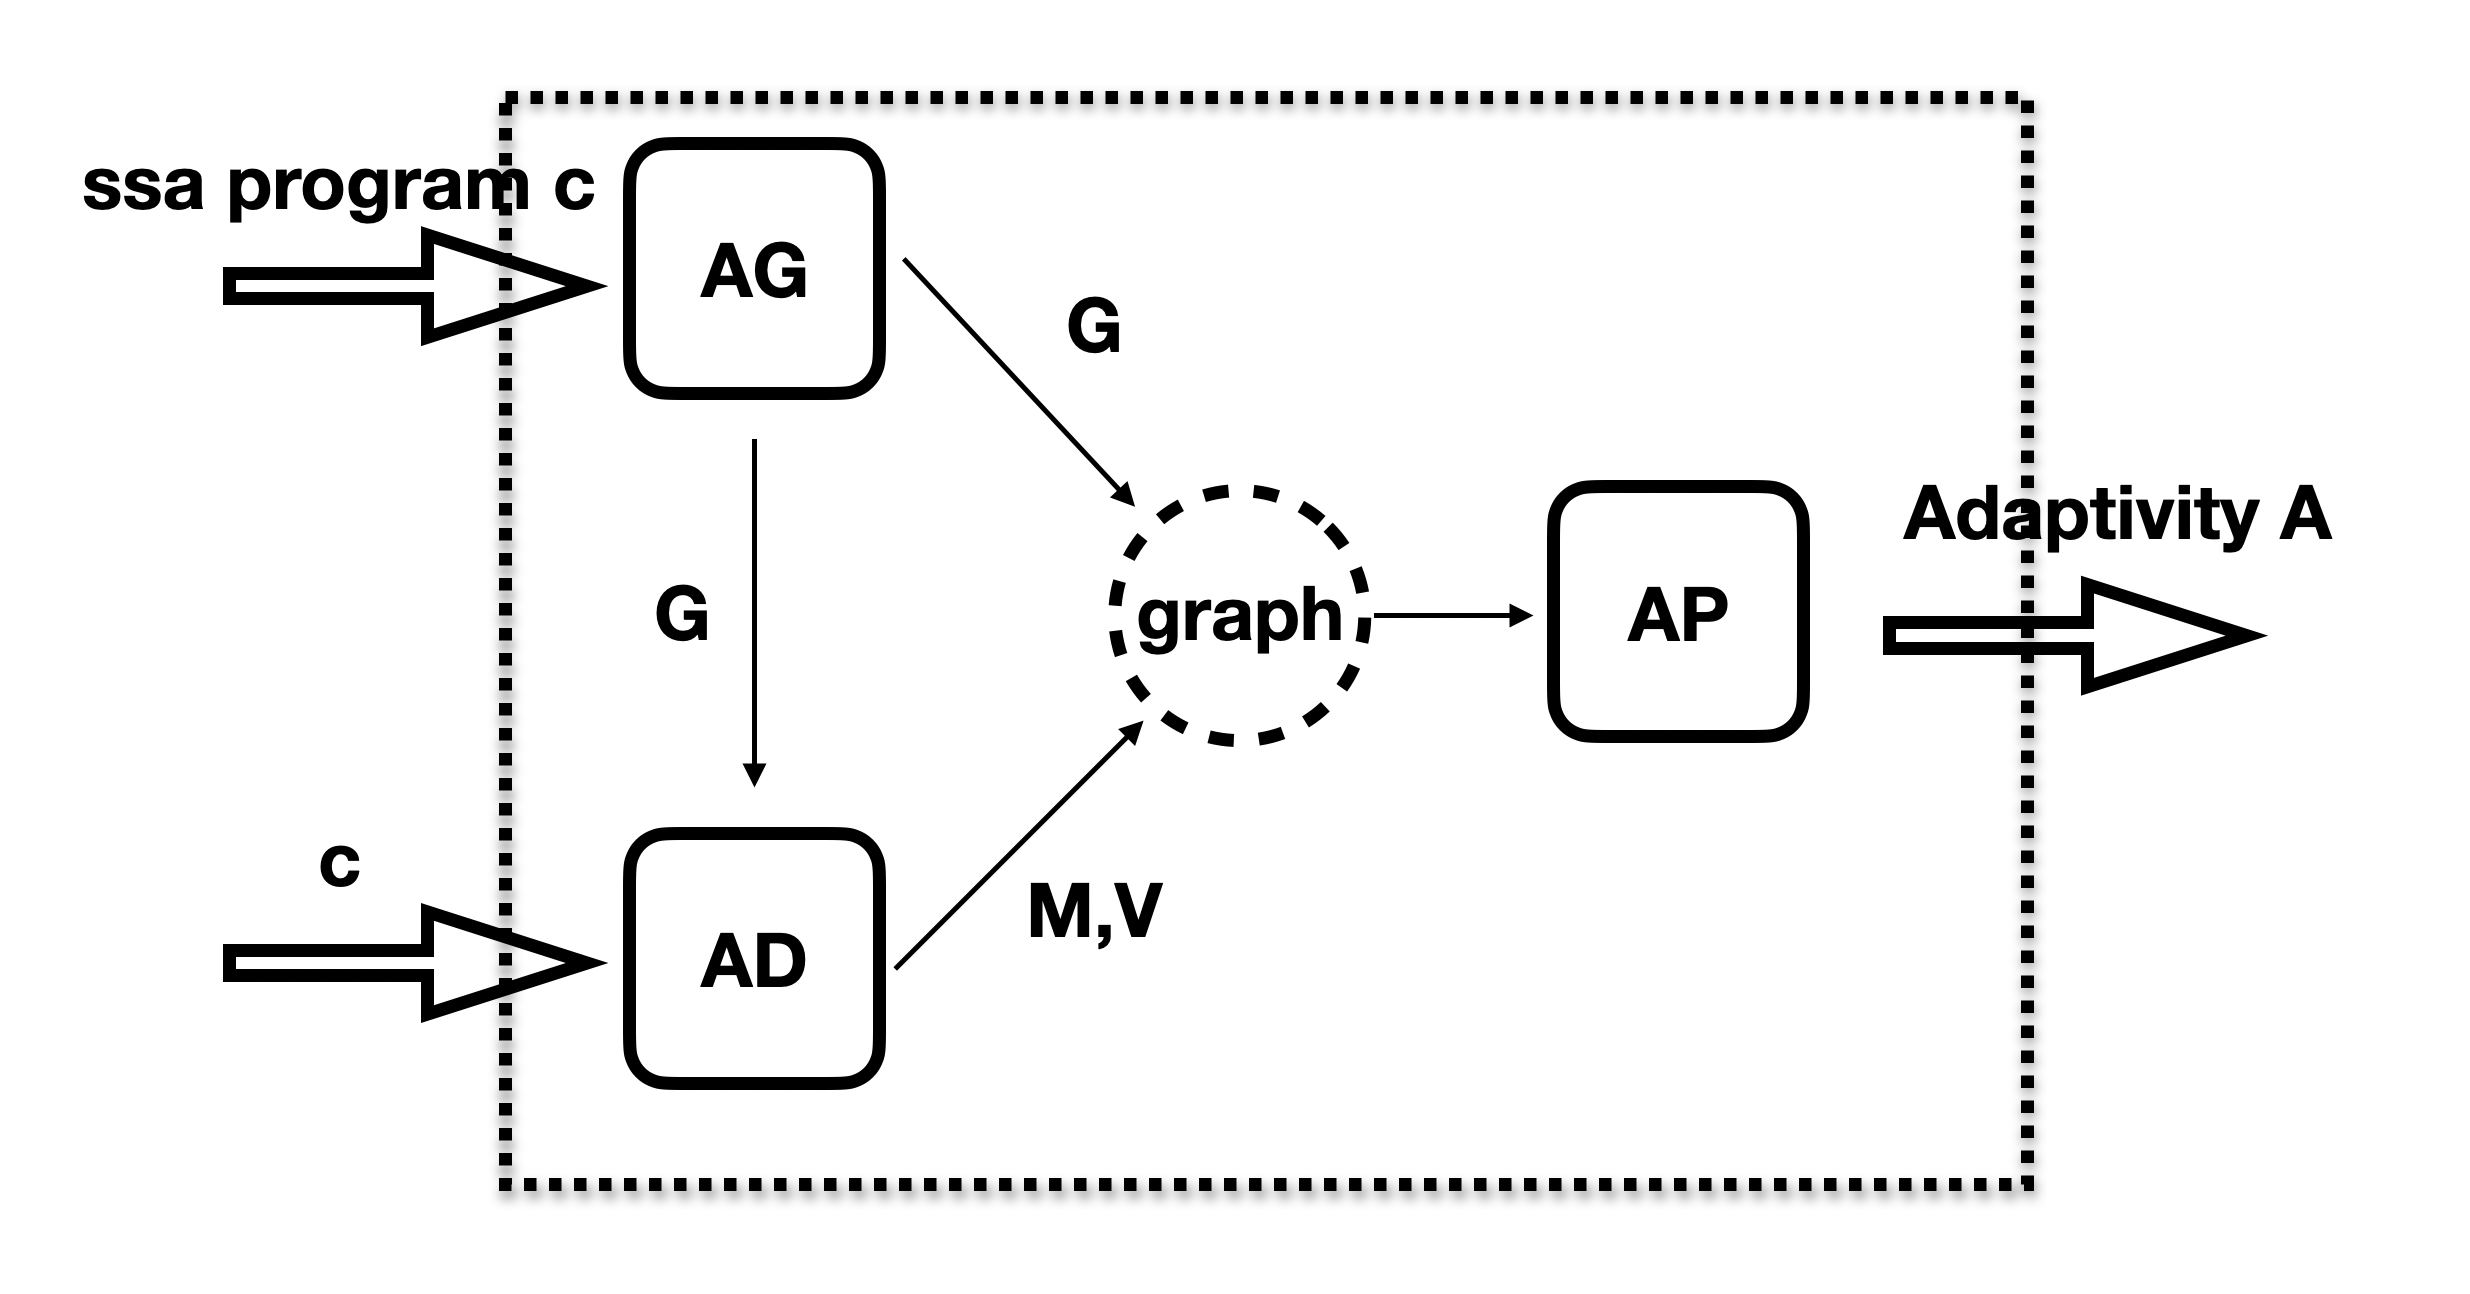
\includegraphics[width=0.7\columnwidth]{adapfun.png}
    \caption{The overview of {\THESYSTEM}}
    \label{fig:adaptfun}
\end{figure}


\subsection{Variable Estimation algorithm}
We first show how $G$ will be collected, through a variable estimating algorithm $\mathsf{AG}$ of the form $\ag{G; w; \ssa{c}}{ G'; w'} $ in Figure~\ref{fig:ag}. The input of $\mathsf{AG}$ is a list of estimated annotated variables $G$ collected before the program $\ssa{c}$, a while map $w$ consistent with previous estimation, a program $\ssa{c}$. The output of the algorithm is the updated global list $G'$, along with the updated while map $w$ for later estimation.   
\begin{figure}
 \begin{mathpar}
\inferrule
{
}
{ \ag{G ;w; \ssa{[\assign {x}{\expr}]^{l}}}{G ++ [\ssa{x}^{(l,w)}];w}
% G ;w; \ssa{[\assign {x}{\expr}]^{l}} \to G ++ [x^{(l,w)}];w 
}
~\textbf{ag-asgn}
\and
\inferrule
{
}
{ \ag{G ;w;  [ \assign{\ssa{x}}{q(\ssa{\expr})}]^{l}}{  G ++ [\ssa{x}^{(l,w)}] ; w} 
}~\textbf{ag-query}
%
\and 
%
\inferrule
{
\ag{G; w; \ssa{c_1}}{  G_1;w_1}
\and 
 \ag{G_1;w ; \ssa{c_2}}{  G_2; w_2}
 \\
 {G_3 = G_2 ++ \ssa{[\bar{x}^{(l,w)}]++ \ssa{[\bar{y}^{(l,w)}]}++ \ssa{[\bar{z}^{(l,w)}]} }}
}
{
\ag{G; w;
[\eif(\ssa{\bexpr},[ \bar{\ssa{x}}, \bar{\ssa{x_1}}, \bar{\ssa{x_2}}] ,[ \bar{\ssa{y}}, \bar{\ssa{y_1}}, \bar{\ssa{y_2}}],[ \bar{\ssa{z}}, \bar{\ssa{z_1}}, \bar{\ssa{z_2}}], \ssa{ c_1, c_2)}]^{l} }{ G_3 ;w}
}~\textbf{ag-if}
%
%
%
\and 
%
\inferrule
{
\ag{G; w; \ssa{c_1}}{ G_1; w_1}
\and 
\ag{G_1;w_1; \ssa{c_2}}{ G_2; w_2}
}
{
\ag{G; w;
\ssa{(c_1 ; c_2)}}{  G_2 ; w_2}
}
~\textbf{ag-seq}
\and 
\inferrule
{
{G_0 = G \quad w_0 =w }
\and
\forall 0 \leq z < N. 
{ \ag{ G_z ++ \ssa{[\bar{x}^{(l, {w_z}+l)}]} ; (w_z+l); \ssa{c}}{ G_{z+1} ; w_{z+1}}  }
\\
{G_f = G_N ++ \ssa{[\bar{x}^{(l, w_N \setminus l)}]} }
\and
{ \ssa{\aexpr} =  {N}  }
}
{\ag{G; w; [\eloop ~ \ssa{\aexpr}, n, [\bar{\ssa{x}}, \bar{\ssa{x_1}}, \bar{\ssa{x_2}}] ~ \edo ~ \ssa{c}]^{l} }{ G_f; w_N\setminus l }
}~\textbf{ag-loop}
% \and 
% \inferrule
% {
% \Gamma \vdash^{(i,i+a )}_{M, V} c 
% }
% {\Gamma \vdash^{(i, i+ N*a)}_{M_{i,a}^N(f), V_{i, a}^N} 
% \ewhile([\bexpr]^l,   c) : \phi \Rightarrow \psi
% }~\textbf{while}
% %
% \and
% %
% \inferrule
% {
% }
% { \ag{ G;w; [ \eswitch(\ssa{\expr}, \ssa{x},(\ssa{v_j} \rightarrow \ssa{q_j} ) )]^{l} } { G ++ [\ssa{x}^{(l, w)}] ; w} }
% ~\textbf{switch}
\end{mathpar}
 \caption{The algorithm $\mathsf{AG}$ }
    \label{fig:ag}
\end{figure}
The assignment is the source of variables $\mathsf{AG}$ estimates, in the case $\textbf{ag-asgn}$ and $\textbf{ag-query}$, the output global list is extended by $\ssa{x}^{(l,w)}$. When it comes to the if command in the rule $\textbf{ag-if}$, variables assigned in the then branch $\ssa{c_1}$, as well as the variables assigned in the else branch $\ssa{c_2}$, and the new generated variables $\bar{\ssa{x}},\bar{\ssa{y}},\bar{\ssa{z}}$ in $ [ \bar{\ssa{x}}, \bar{\ssa{x_1}}, \bar{\ssa{x_2}}] ,[ \bar{\ssa{y}}, \bar{\ssa{y_1}}, \bar{\ssa{y_2}}],[ \bar{\ssa{z}}, \bar{\ssa{z_1}}, \bar{\ssa{z_2}}]$. The sequence is standard by accumulating the predicted variables in the two commands $\ssa{c_1}$ and $\ssa{c_2}$ in a sequence $\ssa{c_1;c_2}$. The loop considers the loop iterations as well by assuming the loop counter $\ssa{\aexpr}$ to be certain natural number $N$ in the rule $\textbf{ag-loop}$. The algorithm counts the assigned variables in every iteration, including those new assigned variables in $\bar{\ssa{x}}$, those variables assigned in the body $\ssa{c}$, with the appropriate annotation showing the iteration number of the variables.      


\subsection{Matrix and Vector based algorithm}
We have a global list $G$ after the first scan of the ssa programs $\ssa{c}$. We develop a matrix and vector based approach based on the global list $G$ to get an estimated upper bound on the adaptivity of the program.  In this approach, a matrix is constructed according to those estimated annotated variables from the global list, in which every row and every column corresponds to the unique variable in $G$ by position. To be precise, in this matrix, $0$ means no dependency while non-zero value in the matrix shows may-dependency between corresponding variables. If the value of $M[i][j]$ in the matrix $M$ is greater than zero, we know annotated variable $G[i]$ may depend on $G[j]$. A vector $V$ has the same size as $G$ and it records whether the corresponding variable $G[i]$ is assigned with a query request. $V[i] =1$ means assigned with a query request and  otherwise $V[i]=0$. We call this algorithm which tracks may-dependency in the ssa programs and query information, $\mathsf{AD}$. The algorithm of the form $ \ad{\Gamma; \ssa{c} ;i }{ M; V;  i' } $, the input is a tuple consisting of three elements: (1) a one-row-N-column matrix $\Gamma$ storing the dependency from previous program, it is used when handling the if command. (2) the ssa program $\ssa{c}$ to be analyzed (3) an index $i$ specifying the location of the first assigned variable of the program $\ssa{c}$ in the global list $G$. The output of $\mathsf{AD}$ also consists of three elements ; (1) A matrix $M$ showing the may-dependency in $\ssa{c}$ (2) A vector $V$ records the query requests in $\ssa{c}$ (3) the index $i'$ that refers to the next position of the last assigned variable in $\ssa{c}$, if exists. The existence of the index $i'$ helps to locate the first assigned variable if we need to analyze programs after $\ssa{c}$.  

We first define some functions which use the indices in $G$. 
The function $\mathsf{L(i)}$ generates one-column-N-rows  matrix, where only the $i-th$ row is $1$ and all the other rows are $0$. This function is used to locate the right row when calculate the matrix when analyzing assignment and query. 

The function $\mathsf{R(e, i)}$ generates a one-row-N-column matrix. For every variable used in $e$, it finds the corresponding index $i$ in $G$ so that $G[i]$ maps to the variable and mark the $i$th column as $1$. If it is not found, we do not mark. When we say $G[i]$ maps to a target variable, we take off the annotation of $G[i]$ and check if the left variable is the same as the target variable. To handle loop, for instance, a variable $y$ appears many times in $G$, but with different annotations(iteration numbers), the argument $i$ helps to find most recent assignment variable $y$ before the index $i$ in $G$. It is still used when analyzing assignment and query. Thanks to our ssa language, our choice of the most recent assigned variable is reasonable because the variable used in the loop refers to the most recent assignment and every variable is uniquely assigned in its ssa form. 

We define $M_1;M_2$ to combine two matrix, where $M_1 + M_2$ is the standard sum of two matrix.
\[
M_1 ; M_2  :=  M_2 \cdot M_1 + M_1 + M_2 
\]
And define the operator $\uplus$ to combine two vectors.
\[
V_1 \uplus V_2  :=  \left\{
\begin{array}{ll}
1 & (V_1[i] = 1 \lor V_2[i] = 1) \land i = 1, \cdots, N \land |V_1| = |V_2|\\
0 & o.w.
\end{array}\right.
\]
For the sake of brevity, we also define some annotations as follows. We show how the algorithm $\mathsf{AD}$ handles the extra part $[ \bar{\ssa{x}}, \bar{\ssa{x_1}},\bar{\ssa{x_2}} ] $ in the if and loop commands. First, we give a unique name for variables in lists $\bar{\ssa{x}}, \bar{\ssa{x_1}}, \bar{\ssa{x_2}}$ respectively, as follows: {$ \forall 0 \leq z < |\bar{\ssa{x}}|. \bar{\ssa{x}}(z) = \ssa{x_z}, \bar{\ssa{x_1}}(z) = \ssa{x_{1z}}, \bar{\ssa{x_2}}(z) = \ssa{x_{2z}} $ }. And then we treat every tuple $(\ssa{x_z},\ssa{x_{1z}},\ssa{x_{2z}} )$ in $[\bar{\ssa{x}}, \bar{\ssa{x_1}}, \bar{\ssa{x_2}} ]$ as the simple may dependency case : $\ssa{x_z}$ may depend on both $ \ssa{x_{1z}}$ and $\ssa{x_{2z}}$, just like $ \assign{\ssa{x_z} }{\ssa{x_{1z}} + \ssa{x_{2z}} }$, defined as follows. 
$
 \ad{\Gamma; [\bar{\ssa{x}}, \bar{\ssa{x_1}}, \bar{\ssa{x_2}} ] ; i }{ M; V_{\emptyset}; i + |\bar{\ssa{x}}| } 
  \triangleq { \forall 0 \leq z < |\bar{\ssa{x}}|.
  \ad{\Gamma;\assign{\ssa{x_z} }{\ssa{x_{1z}} + \ssa{x_{2z}} }; i+z }{ M_{x_z};  V_{\emptyset}; i+z+1} }$
   where $M = \sum_{o \leq z < |\bar{\ssa{x}}| }M_{x_z} $.
% \framebox{$ \ad{\Gamma; \ssa{c} ; i_1){M;V;i_2} $}
%
\begin{figure}
\begin{mathpar}
\inferrule
{M = \mathsf{L}(i) * ( \mathsf{R}(\ssa{\expr},i) + \Gamma )
}
{
 \ad{\Gamma;[\assign {\ssa{x}}{\ssa{\expr}} ]^{l}; i }{M; V_{\emptyset}; i+1 }
% \Gamma \vdash_{M, V_{\emptyset}}^{(i, i+1)} [\assign {\ssa{x}}{\ssa{\expr}} ]^{l}
}
~\textbf{ad-asgn}
\and
\inferrule
{M = \mathsf{L}(i) * ( \mathsf{R}(\ssa{\expr},i) + \Gamma )
\\
V= \mathsf{L}(i)
}
{ 
\ad{\Gamma;[ \assign{\ssa{x}}{q(\ssa{\expr})} ]^{l} ; i }{M;V;i+1}
%  \vdash^{(i, i+1)}_{M, V} [ \assign{\ssa{x}}{q(\ssa{\expr})} ]^{l} 
}~\textbf{ad-query}
%
\and 
%
\inferrule
{
{\ad{\Gamma + \mathsf{R}(\ssa{\bexpr}, i_1); \ssa{c_1} ; i_1 }{ M_1;V_1;i_2 }}
% \Gamma + \mathsf{R}(\bexpr, i_1) \vdash^{(i_1, i_2)}_{M_1, V_1} \ssa{c_1} 
% : \Phi \land \bexpr \Rightarrow \Psi
\and 
{\ad{\Gamma + \mathsf{R}(\ssa{\bexpr}, i_1);\ssa{c_2} ; i_2 }{ M_2; V_2 ;i_3}}
% \Gamma + \mathsf{R}(\ssa{\bexpr}, i_1) \vdash^{(i_2, i_3)}_{M_2, V_2} \ssa{c_2} 
% : \Phi \land \neg \bexpr \Rightarrow \Psi
\\
% { \forall 0 \leq j < |\bar{x}|. \bar{x}(j) = x_j, \bar{x_1}(j) = x_{1j}, \bar{x_2}(j) = x_{2j}  }
{\ad{\Gamma; [ \bar{\ssa{x}}, \bar{\ssa{x_1}}, \bar{\ssa{x_2}}]; i_3 }{ M_x; V_{\emptyset}; i_3+|\bar{\ssa{x}}| }}
%
\and
%
{\ad{\Gamma; [ \bar{\ssa{y}}, \bar{\ssa{y_1}}, \bar{\ssa{y_2}}]; i_3+|\bar{\ssa{x}}| }{ M_y; V_{\emptyset}; i_3+|\bar{\ssa{x}}|+|\bar{\ssa{y}}| }}
%
\\
%
{\ad{\Gamma; [ \bar{\ssa{z}}, \bar{\ssa{z_1}}, \bar{\ssa{z_2}}]; i_3+|\bar{\ssa{x}}|+ |\bar{\ssa{y}}|}{ M_y; V_{\emptyset}; i_3+|\bar{\ssa{x}}|+|\bar{\ssa{y}}| + |\bar{\ssa{z}}| }}
% { \forall 0 \leq j < |\bar{x}|.  \Gamma \vdash_{M_{x_j}, V_{\emptyset}}^{i_3+j, i_3+j+1 } x_j \leftarrow x_{1j} + x_{2j} }
% \and
% { \forall 0 \leq j < |\bar{y}|.  \Gamma \vdash_{M_{y_j}, V_{\emptyset}}^{i_3+|\bar{x}|+j, i_3+|\bar{x}|+j+1 } y_j \leftarrow y_{1j} + y_{2j} }
% \\
% { \forall 0 \leq j < |\bar{z}|.  \Gamma \vdash_{M_{z_j}, V_{\emptyset}}^{i_3+|\bar{x}|+|\bar{y}|+j, i_3+|\bar{x}|+|\bar{y}|+j+1 } z_j \leftarrow z_{1j} + z_{2j} }
\\
{M = (M_1+M_2)+ M_x+M_y +M_z }
}
{
\Gamma \vdash^{(i_1, i_3+|\bar{x}|+|\bar{y}|+|\bar{z}|)}_{M, V_1 \uplus V_2 } 
[\eif(\ssa{\bexpr},[ \bar{\ssa{x}}, \bar{\ssa{x_1}}, \bar{\ssa{x_2}}] ,[ \bar{\ssa{y}}, \bar{\ssa{y_1}}, \bar{\ssa{y_2}}] , [ \bar{\ssa{z}}, \bar{\ssa{z_1}}, \bar{\ssa{z_2}}] , \ssa{ c_1, c_2)}]^{l}
}~\textbf{ad-if}
%
%
%
\and 
%
\inferrule
{
{\ad{\Gamma; \ssa{c_1} ; i_1 }{ M_1 ; V_1; i_2 }  }
% \Gamma \vdash^{(i_1, i_2)}_{M_1, V_1} \ssa{c_1} 
% : \Phi \Rightarrow \Phi_1
\and 
{\ad{\Gamma;\ssa{c_2}; i_2}{M_2; V_2 ;i_3 }}
% \Gamma \vdash^{(i_2, i_3)}_{M_2, V_2} \ssa{c_2} 
% : \Phi_1 \Rightarrow \Psi 
}
{
\ad{\Gamma ; (\ssa{c_1 ; c_2} ) ; i_1}{(M_1 {;} M_2) ; V_1 \uplus V_2 ; i_3  }
% \Gamma \vdash^{(i_1, i_3)}_{M_1 {;} M_2, V_1 \uplus V_2}
% \ssa{c_1 ; c_2} 
% : \Phi \Rightarrow \Psi
}
~\textbf{ad-seq}
\and 
\inferrule
{
B= |\ssa{\bar{x}}| \and {A = |\ssa{c}|}
% \and
% {\Gamma \vdash^{(i, i+B)}_{M_{10}, V_{10}} [\bar{\ssa{x}}, \bar{\ssa{x_1}}, \bar{\ssa{x_2}}] }
% \and
% {\Gamma \vdash^{(i+B,i+B+A )}_{M_{20}, V_{20}} \ssa{c} 
% }
\\
\forall 0 \leq j < N. 
{\ad{\Gamma;[\bar{\ssa{x}}, \bar{\ssa{x_1}}, \bar{\ssa{x_2}}]; i+ j*(B+A) }{M_{1j};V_{1j}; i+B+j*(B+A) }}
% {\Gamma \vdash^{(i+j*(B+A), i+B+j*(B+A))}_{M_{1j}, V_{1j}}  } [\bar{\ssa{x}}, \bar{\ssa{x_1}}, \bar{\ssa{x_2}}]
\\
{
\ad{\Gamma;\ssa{c} ; i+B+j*(B+A)  }{M_{2j}; V_{2j}; i+B+A+j*(B+A) }
% \Gamma \vdash^{(i+B+j*(B+A),i+B+A+j*(B+A) )}_{M_{2j}, V_{2j}} \ssa{c} 
% : \Phi \land e_n = \lceil{z+1}\rceil \Rightarrow \Psi 
}
\\
{
\ad{\Gamma ; [\bar{\ssa{x}}, \bar{\ssa{x_1}}, \bar{\ssa{x_2}}] ; i+N*(B+A) }{M; V ;i+N*(B+A)+B}
% \Gamma \vdash^{(i+N*(B+A) ,i+N*(B+A)+B )}_{M, V} [\bar{\ssa{x}}, \bar{\ssa{x_1}}, \bar{\ssa{x_2}}]
% : \Psi \Rightarrow \Phi \land e_N = \lceil{z}\rceil 
}
\\
{ \ssa{\aexpr} =  {N}  }
\and
{M' = M+ \sum_{0 \leq j <N}( M_{1j}+M_{2j})  }
\and
{V' = V \uplus \sum_{0 \leq j <N}( V_{1j} \uplus V_{2j})  }
}
{\Gamma \vdash^{(i, i+N*(B+A)+B   )}_{M', V'} 
[\eloop ~ \ssa{\aexpr}, 0, [\bar{\ssa{x}}, \bar{\ssa{x_1}}, \bar{\ssa{x_2}}] ~ \edo ~ \ssa{c}]^{l}
% : \Phi \land \expr_N = \lceil { N} \rceil \Rightarrow \Phi \land \expr_N = \lceil{0}\rceil
}~\textbf{ad-loop}
% \and 
% \inferrule
% {
% \Gamma \vdash^{(i,i+a )}_{M, V} c 
% }
% {\Gamma \vdash^{(i, i+ N*a)}_{M_{i,a}^N(f), V_{i, a}^N} 
% \ewhile([\bexpr]^l,   c) : \phi \Rightarrow \psi
% }~\textbf{while}
% %
% \and
% %
% \inferrule
% { \Gamma + \mathsf{R}(\expr,i) \vdash^{(i, i+1)}_{M, V} \assign{ x}{q_j} 
% % : \Phi \Rightarrow \Psi
% \\
% j \in \{1, \dots, N\}     }
% {\Gamma \vdash^{(i, i+1)}_{ M,V } 
% [\eswitch(\ssa{\expr}, \ssa{x},(v_j \rightarrow q_j ) ]^{l}
% % : \Phi \Rightarrow \Psi 
% }
% ~\textbf{switch}
% %
% \and
% %
% \inferrule
% { 
% \vDash 
% \Phi \Rightarrow \Phi'  
% \and
% \Gamma \vdash^{(i_1, i_2)}_{(M',V')} c : \Phi' \Rightarrow \Psi'
% \and
% \vDash \Psi' \Rightarrow \Psi
% \and 
% \Phi \vDash M' \leq M
% \and 
% \Phi \vDash V' \leq V
% }
% {\Gamma \vdash^{(i_1, i_2)}_{(M,V)} c 
% : \Phi \Rightarrow \Psi
% }
% ~\textbf{conseq}
\end{mathpar}
    \caption{The algorithm AD}
    \label{fig:algo_ad}
\end{figure}
One of the key idea under algorithm $\mathsf{AD}$ is to track the indices $i$,$i'$ both in the input and output to synchronize with its previous algorithm $\mathsf{AG}$. The index in $\mathsf{AD}$ increases as the same way as the global list expands after the analysis of a program $\ssa{c}$, which helps $\mathsf{AD}$ record the dependency relation from the program $\ssa{c}$ in the right place of the matrix. For example, in the case $\textbf{ad-asgn}$ and $\textbf{ad-query}$, the index increases by 1, which corresponds to their counterparts of algorithm $\textbf{AG}$. The if and loop commands have the extra part $ [\bar{\ssa{x}}, \bar{\ssa{x_1}}, \bar{\ssa{x_2}}] $ and we find that the output index increases by also considering this part as we do in collecting the global list.  

Another interesting point is the construction of the matrix. The fundamental case is the assignment and query cases. We use a function $L(i)$ to generate a N-row-one-column matrix $L$ to guarantee the resulting matrix only has non-zeros at row $i$. The intuition behind is that one single assignment or query request can only reveal the dependency of its assigned variable (corresponding to one row of the matrix) to the variables used on the right hand sides. Thanks to the index $i$, we know which row this assignment should be in the matrix. The function $\mathsf{R}(\ssa{\expr},i)$ gets a one-row-N-column matrix marking the variables used in the right hand side. The $\Gamma$ is designed for the if command and we will discuss it later. We can see one simple example $sa$ to get a taste.     
\[
sa \triangleq
\begin{array}{l}
    \left[x_1 \leftarrow 2 \right]^1; \\
    \left[x_2 \leftarrow x_1 + 2 \right]^2 ; \\
    \left[x_3 \leftarrow x_1 + x_2 \right]^3
\end{array}
\]
In the program $sa$, only simple assignment is involved. When we assume $\Gamma$ is empty, for the assignment at line $3$, the matrix is built as follows.
\[
\textbf{line3:} ~~
 \left[x_3 \leftarrow x_1 + x_2 \right]^3 :
 ~~~
\begin{blockarray}{cc}
\begin{block}{c[c]}
 x_1 & 0   \\
 x_2 & 0 \\
 x_3 & 1 \\
\end{block}
\end{blockarray}
*
\begin{blockarray}{ccc}
x_1 & x_2 & x_3 \\
\begin{block}{[ccc]}
1 & 1 & 0 \\
\end{block}
\end{blockarray}
= 
\begin{blockarray}{cccc}
& x_1 & x_2 & x_3\\
\begin{block}{c[ccc]}
x_1 & 0 & 0 & 0 \\
x_2 & 1 & 0 & 0 \\
x_3 & 1 & 1 & 0 \\
\end{block}
\end{blockarray}
\]
% a simple example of assignment
% \begin{example}[Simple Assignment]
% \[
% SA \triangleq
% \begin{array}{l}
%     \left[x_1 \leftarrow 2 \right]^1; \\
%     \left[x_2 \leftarrow x_1 + 2 \right]^2 ; \\
%     \left[x_3 \leftarrow x_1 + x_2 \right]^3
% \end{array}
% \]
% %
% %
% \[
%  \textbf{line2:} ~~
%  \left[x_2 \leftarrow x_1 + 2 \right]^2 :
%  ~~~
% \begin{blockarray}{cc}
% \begin{block}{c[c]}
%  x_1 & 0   \\
%  x_2 & 1 \\
%  x_3 & 0 \\
% \end{block}
% \end{blockarray}
% *
% \begin{blockarray}{ccc}
% x_1 & x_2 & x_3 \\
% \begin{block}{[ccc]}
% 1 & 0 & 0 \\
% \end{block}
% \end{blockarray}
% = 
% \begin{blockarray}{cccc}
% & x_1 & x_2 & x_3\\
% \begin{block}{c[ccc]}
% x_1 & 0 & 0 & 0 \\
% x_2 & 1 & 0 & 0 \\
% x_3 & 0 & 0 & 0 \\
% \end{block}
% \end{blockarray}
% \]
% %
% %
% %
% \[
% \textbf{line3:} ~~
%  \left[x_3 \leftarrow x_1 + x_2 \right]^3 :
%  ~~~
% \begin{blockarray}{cc}
% \begin{block}{c[c]}
%  x_1 & 0   \\
%  x_2 & 0 \\
%  x_3 & 1 \\
% \end{block}
% \end{blockarray}
% *
% \begin{blockarray}{ccc}
% x_1 & x_2 & x_3 \\
% \begin{block}{[ccc]}
% 1 & 1 & 0 \\
% \end{block}
% \end{blockarray}
% = 
% \begin{blockarray}{cccc}
% & x_1 & x_2 & x_3\\
% \begin{block}{c[ccc]}
% x_1 & 0 & 0 & 0 \\
% x_2 & 1 & 0 & 0 \\
% x_3 & 1 & 1 & 0 \\
% \end{block}
% \end{blockarray}
% \]
% %
% \end{example}
 We use a one-row-N-column matrix $\Gamma$ as one of the input of $\mathsf{AD}$, to handle the cases when the control flow diverges in the labelled if command $[\eif(\ssa{\bexpr},[ \bar{\ssa{x}}, \bar{\ssa{x_1}}, \bar{\ssa{x_2}}] ,[ \bar{\ssa{y}}, \bar{\ssa{y_1}}, \bar{\ssa{y_2}}] , [ \bar{\ssa{z}}, \bar{\ssa{z_1}}, \bar{\ssa{z_2}}] , \ssa{ c_1, c_2)}]^{l} $, where the execution of either branch may depend on the conditional guard $\ssa{\bexpr}$. Follow this intuition, the analysis of either branch is supposed to consider the variables used in the conditional $\ssa{\bexpr}$, tracked in $\Gamma$. In the case $\textbf{ad-if}$, we can see the analysis of the two branches $\ssa{c_1}$ and $\ssa{c_2}$ share the same input $\Gamma + \mathsf{R}(\ssa{\bexpr}, i)$ and $\mathsf{R}(\ssa{\bexpr}, i) $ tells the variables assigned before the if command and used in the conditional $\ssa{\bexpr}$.   

We compose the matrix and vectors in the case of sequence in $\textbf{ad-seq}$. The non-zeros or we call it effect range of the matrix and vector is decided by its input and output indices. From the case $\textbf{ad-seq}$, two programs $\ssa{c_1}$ and $\ssa{c_2}$ have disjoint effect ranges $[i_1, i_2)$ and $[i_1,i_3)$, it is safe to combine them without lose information. 

The loop case is handled in a well organized way. We use $B= |\bar{\ssa{x}}|$ and $A= |{\ssa{c}}|$ to estimate the size of variables assigned in $\bar{\ssa{x}}$ and $\ssa{c}$. And  $|\ssa{c}|$ is defined by the help of the algorithm $\mathsf{AG}$, defined as $|\ssa{c}|= |G|$ when $\ag{[];\ssa{c};\emptyset }{ G; \emptyset }$. The algorithm then gets how many iterations $N$ the loop may executes from the loop counter $\ssa{\aexpr}$. For every iteration, it first records the dependency relations between variables in $ [\bar{\ssa{x}}, \bar{\ssa{x_1}}, \bar{\ssa{x_2}}]$ by constructing a corresponding matrix $M_{1j}$ ($j$ is the iteration number) and an empty vector $V_{1j}$, and analyze the loop body $\ssa{c}$ with a resulting matrix $M_{2j}$ and vector $V_{2j}$. We give an extra analysis of those new assigned variables as what $\mathsf{AG}$ does, it works well when the loop is executed ($N = 0$) or not. We know that for all the possible iteration number $j$, $M_{1j}$ and $M_{2j}$ have disjoint effect ranges so we combine them, similar as the vectors $V_{1j}$ and $V_{2j}$.   

Finally, we are able to construct a variable-based weighted dependency graph based on $G$,$M$ and $V$ generated by the framework. The definition of the estimated adaptivity is the weight of the most weighted path in the graph defined as follows. 

\begin{defn}
[Estimated Adaptivity]
Given a program $\ssa{c}$, the global list $G$, and $\ad{\Gamma; \ssa{c}; i_1}{M, V, i_2}$, the weighted dependency graph $G_{ssa}(M, V,G,i_1,i_2) = (Nodes, Edges, Weights)$ is defined as:
\\
Nodes $Vt = \{ G(j) \in \mathcal{LV} \mid i_1 \leq j < i_2 \}$
\\
Edges $E = \{ (G(j_1), G(j_2)) \in \mathcal{LV} \times \mathcal{LV} \mid M[j_1][j_2] \geq 1 \land  i_1 \leq j_1,j_2 < i_2   \}$
\\
 Weights $Wt = \{ (  G(j), 1 ) \in \mathcal{LV} \times \mathcal{N} | i_1 \leq j < i_2 \land V[j] = 1\}
        \cup \{ (  G(j), 0 ) \in \mathcal{LV} \times \mathcal{N} | i_1 \leq j < i_2 \land V[j] = 0 \} $.
        
Adaptivity of the program defined according to the graph is as:
\[
Adapt(M, V,i_1,i_2) := \max_{vt_1, vt_2 \in Vt}\{ \mathsf{Weight}( p(vt_1, vt_2), Wt) \},
\]
where $p(k, l)$ is the path in graph $G_{ssa}(M, V, i_1,i_2)$ starting from $k$ to $l$, $\mathsf{Weight}(p(vt_1,vt_2), Wt)$ get the total sum of weights along the path $p(vt_1,vt_2)$.
\end{defn}        

\subsection{Analysis on two round algorithm}
We show how {\THESYSTEM} analyze the two round algorithm. For the sake of brevity, we conduct the analysis on the simplified two round algorithm $TR^{ssa}$.

% \[
% TR^{ssa}(k) \triangleq
% {
% \begin{array}{l}
%     % \left[j \leftarrow 0 \right]^1 ; \\
%     \clabel{a_1 \leftarrow []}^{1} ; \\
%     \clabel{\assign{j_1}{0} }^{2} ; \\
%     \eloop ~ \clabel{k}^{3} ~ \edo [(j_3, j_1,j_2),(a_3, a_1,a_2)]~ \\
%     \Big(
%     \clabel{ x_1 \leftarrow q(\chi(j_3)\cdot \chi(k))}^{4}  ; \\
%     \clabel{ \assign{j_2}{j_3+1} }^{5} ;\\
%     \clabel{a_2 \leftarrow x_1 :: a_3}^{6}       \Big);\\
%     \clabel{l_1 \leftarrow q(\mathrm{sign}\big (\sum_{i\in [k]} \chi(i)\times\ln\frac{1+a_3[i]}{1-a_3[i]} \big ))}^{7}\\
% \end{array}
% }
% \]
{\THESYSTEM} first runs the algorithm $\mathsf{AG}$ to generate the global list $G$. We assume the input $k=2$ and have the following.

\[G_{k=2} = \left[
  {a_1}^{(1,\emptyset)} , {a_3}^{(2,[2:1])} , {x_1}^{(3,[2:1])} , {a_2}^{(4,[2:1])} ,  {a_3}^{(2,[2:2])} , {x_1}^{(3,[2:2])} , {a_2}^{(4,[2:2])} , {a_3}^{(2,\emptyset)} , {l_1}^{(5,\emptyset)}   \right] \]
% \[G_{k=2} = \left[ \begin{array}{l}
%      {a_1}^{(1,\emptyset)} , {j_1}^{(2,\emptyset)}, {j_3}^{(3,[2:1])} , {a_3}^{(3,[2:1])} , {x_1}^{(4,[2:1])} ,{j_2}^{(5,[2:1])} ,
%   {a_2}^{(6,[2:1])},  \\
%     {j_3}^{(3,[2:2])} , {a_3}^{(3,[2:2])} , {x_1}^{(4,[2:2])} ,{j_2}^{(5,[2:2])} ,
%   {a_2}^{(6,[2:2])},
%   {j_3}^{(3,\emptyset)} , {a_3}^{(3,\emptyset)} ,
%   {l_1}^{(7,\emptyset)} \\  
% \end{array}
%      \right] \]
 We denote $a_1^{1}$ short for ${a_1}^{(1,\emptyset)}$ and ${a_3}^{(2,1)}$ short for ${a_3}^{(2,[2:1])}$. Then the resulting matrix $M_{tr}$ and $V_{tr}$ of the algorithm $\mathsf{AD}$ as follows.
 
{ \tiny
 \[
M_{tr} =  \left[ \begin{matrix}
 & a_1^{1} & a_3^{(2,1)} & x_1^{(3,1)} & a_2^{(4,1)}  & a_3^{(2,2)} & x_1^{(3,2)} & a_2^{(4,2)} & a_3^{2} & l_1^{5}\\
 a_1^{1} & 0 & 0 & 0 & 0 & 0 & 0 & 0 &0 &0 \\
a_3^{(2,1)} & 1 & 0 & 0 & 0 & 0 & 0 & 0&0&0\\
x_1^{(3,1)} & 0 & 0 & 0 & 0 & 0 & 0& 0& 0 &0\\
a_2^{(4,1)} & 0 & 1 & 1 & 0 & 0 & 0 & 0& 0&0\\
a_3^{(2,2)} & 1 & 0 & 0 & 1 & 0 & 0 & 0 & 0&0 \\
x_1^{(3,2)} & 0 & 0 & 0 & 0 & 0 & 0 & 0& 0&0\\
a_2^{(4,2)} & 0 & 0 & 0 & 0 & 1 & 1 & 0& 0&0\\
a_3^{2} & 1 & 0 & 0 & 0 & 0 & 0 & 1& 0&0\\
l_1^{5} & 0 & 0 & 0 & 0 & 0 & 0 & 0 & 1 &0 \\
 \end{matrix} \right] 
~ , V_{tr} = \left [ \begin{matrix}
a_1^{1} &  0 \\
a_3^{(2,1)} & 0 \\
x_1^{(3,1)} & 1 \\
a_2^{(4,1)} &  0 \\
a_3^{(2,2)} & 0 \\
x_1^{(3,2)} & 1 \\
a_2^{(4,2)} &  0 \\
a_3^{2} &  0 \\
l_1^{5} &  1 \\
\end{matrix} \right ]
\]
}
%% a graph is better here

\subsection{ Soundness of {\THESYSTEM}}
We would like to show that the query-based dependency graph generated from the trace of the execution of the target ssa program is a subgraph of the variable-based dependency graph predicted from our algorithm ${\THESYSTEM}$, and the query requested during the execution is also bounded by an estimation from our algorithm.

We first give a definition of subgraph of a query-based dependency graph with respect to a variable-based dependency graph.
\begin{defn}
[Subgraph]
Given a query-based dependency graph $G_{s} = (V_1, E_1)$, a variable-based dependency graph $G_{ssa} = (V_2, E_2)$, $G_{s} \subseteq G_{ssa}$ iff:\\
$\exists f$ so that \\
1. for every $v \in V_1$, $f(v) \in V_2$. 
\\
2. $\forall e=(v_i, v_j) \in E_1$, there exists a path 
% $g(e)$ 
from $f(v_i)$ to $f(v_2)$ in $G_{ssa}$.
\end{defn}

Then we show the soundness of {\THESYSTEM}. In the theorem, we use some definition. $G \vDash M, V$ says that $G$ and $M$, $V$ have the corresponding size. $G; w \vDash (\ssa{c}, i_1,i_2)$ checks if the variables assigned in $\ssa{c}$ calculated by $\mathsf{AG}$ matches the variables in $G$ from index $i_1$ to $i_2$.

\begin{thm}
[Soundness of {\THESYSTEM}]
Given $ \ad{\Gamma; \ssa{c}; i_1 }{M; V;i_2}$,  for any global list $G$,  loop maps $w$ such that $G ;w \vDash (\ssa{c}, i_1, i_2) \land G \vDash (M,V)$. $K$ is the number of queries inquired during the execution of the piece of program $\ssa{c}$ and |V| gives the number of non-zeros in $V$. 
% $|.|_{low} $ is the annotation erasure, which turns a ssa form program $\ssa{c}$ to its low-level version.
Then,
\[
K \leq |V| \land \forall D, \ssa{m}. G_{s}(\ssa{c},D,\ssa{m},w) \subseteq G_{ssa}(M, V,G,i_1, i_2)
\]      
\end{thm}


\section{More examples}
The two round strategy works well in our framework, we explore further to look at an advanced adaptive data analysis algorithm - multiple round algorithm.
\begin{example}[Two Round Algorithm]
    \[
    %
        \kw{twoRounds(k)} \triangleq
    \begin{array}{l}
           \clabel{ a \leftarrow []}^{1} ; \\
            \clabel{\assign{j}{k} }^{2} ; \\
            \ewhile ~ \clabel{j > 0}^{3} ~ \edo ~ \\
            \Big(
             \clabel{\assign{x}{\query(\chi[k - j]\cdot \chi[k])} }^{4}  ; \\
             \clabel{\assign{j}{j-1}}^{5} ;\\
            \clabel{a \leftarrow x :: a}^{6}       \Big);\\
            \clabel{l \leftarrow (\mathrm{sign}\big (\sum_{i\in [k]} \chi[i]\times\ln\frac{1+a[i]}{1-a[i]} \big ))}^{7}\\
        \end{array}
    \]
    %
    \begin{algorithm}
    \footnotesize
    \caption{A two-round analyst strategy for random data (The example in  \cite{dwork2015preserving})}
    \label{alg:twoRound}
    \begin{algorithmic}
    \REQUIRE Mechanism $\mathcal{M}$ with a hidden data set $D \in \{-1,+1\}^{n\times (k+1)} \subset \dbdom$.
    \STATE  {\bf for}\ $j\in [k]$\ {\bf do}.  
    \STATE \qquad {\bf define} $q_j(d)=d(j)\cdot d(k)$ where $d \in \{D(i) ~|~ i = 0, \cdots, n\} \subseteq \{-1,+1\}^{k+1}$.
    \STATE \qquad {\bf let} $a_j=\mathcal{M}(q_j)$ 
    \STATE \qquad \COMMENT{In the line above, $\mathcal{M}$ computes approx. the exp. value  of $q_j$ over $D$. So, $a_j\in [-1,+1]$.}
    \STATE {\bf define} $q_{k}(d)= d(k) \cdot \mathrm{sign}\big (\sum_{i\in [k]} x(i) \cdot \ln\frac{1+a_i}{1-a_i} \big )$ where $x\in \{-1,+1\}^{k+1}$.
    \STATE\COMMENT{In the line above,  $\mathrm{sign}(y)=\left \{ \begin{array}{lr} +1 & \mathrm{if}\ y\geq 0\\ -1 &\mathrm{otherwise} \end{array} \right . $.}
    \STATE {\bf let} $a_{k+1}=\mathcal{M}(q_{k+1})$
    \STATE\COMMENT{In the line above,  $\mathcal{M}$ computes approx. the exp. value  of $q_{k+1}$ over $X$. So, $a_{k+1}\in [-1,+1]$.}
    \RETURN $a_{k+1}$.
    \ENSURE $a_{k+1}\in [-1,+1]$
        % \ENSURE 
    \end{algorithmic}
    \end{algorithm}
    %
%
    \end{example}

\begin{example}[Multiple Round Algorithm]
%
\[
%
\kw{multipleRounds(k, c)} \triangleq
\begin{array}{l}
     \left[j \leftarrow k \right]^1 ; \\
    \left[I \leftarrow [] \right]^2; \\
    \ewhile ~ \clabel{j > 0}^{3} ~ \edo ~ \\
    \Big(
    \clabel{\assign{j}{j-1}}^{4} ;\\
    \left[p \leftarrow c \right]^5; \\
    \left[ a \leftarrow \query (\chi[I]) \right]^6;\\
    \left[I \leftarrow \mathrel{\mathsf{update}} ( {I}, (a, p))  \right]^7
    \Big) 
\end{array}
\]
%
\begin{algorithm}
\footnotesize
\caption{A multi-round analyst strategy for random data base \cite{dwork2015preserving}}
\label{alg:multiRound}
\begin{algorithmic}
\REQUIRE Mechanism $\mathcal{M}$ with a hidden state $X\in [N]^{n}$ sampled u.a.r., control set size $c$
\STATE Define control dataset $C = \{0,1, \cdots, c - 1\}$
\STATE Initialize $Nscore(i) = 0$ for $i \in [N]$, $I = \emptyset$ and $Cscore(C(i)) = 0$ for $i \in [c]$
\STATE  {\bf for}\ $j\in [k]$\ {\bf do} 
\STATE \qquad {\bf let} $p=\uniform(0,1)$ 
\STATE \qquad {\bf define} $q (x) = \bernoulli ( p )$ .
\STATE \qquad {\bf define} $qc (x) = \bernoulli ( p )$ .
\STATE \qquad {\bf let} $a = \mathcal{M}(q)$ 
\STATE \qquad {\bf for}\ $i \in [N]$\ {\bf do}
\STATE \qquad \qquad $Nscore(i) = Nscore(i) + (a - p)*(q (i) - p)$ if $i \notin I$
\STATE \qquad {\bf for}\ $i \in [c]$\ {\bf do}
\STATE \qquad \qquad $Cscore(C(i)) = Cscore(C(i)) + (a - p)*(qc (i) - p)$
\STATE \qquad {\bf let} $I = \{i | i\in [N] \land Nscore(i) > \max(Cscore)\}$
\STATE \qquad {\bf let} $D = D \setminus I$ 
\RETURN $D$.
\end{algorithmic}
\end{algorithm}
%
\[
%
\kw{multipleRounds(k, c, N)} \triangleq
\begin{array}{l}
    \clabel{\assign{j}{N}}^0 ; \\
     \clabel{\assign{cs}{0}}^1; \\
     \clabel{\assign{ns}{0}}^2; \\
     \clabel{\assign{I}{0}}^3; \\
     \ewhile ~ \clabel{j > 0}^{4} ~ \edo ~ \\
     \Big(
     \clabel{\assign{j}{j-1}}^{5} ;\\
     \clabel{\assign{cs}{0 + cs}}^6; \\
     \clabel{\assign{ns}{0 + ns}}^7
     \Big); \\
     \clabel{\assign{w}{k}}^{8} ;\\
     \ewhile ~ \clabel{w > 0}^{9} ~ \edo ~ \\
    \Big(
    \clabel{\assign{w}{w-1}}^{10} ;\\
    \left[p \leftarrow c \right]^{11}; \\
    \left[q \leftarrow c \right]^{12}; \\
    \left[ a \leftarrow \query (\chi[I]) \right]^{13};\\
    \clabel{\assign{i}{N}}^{14} ; \\
    \ewhile ~ \clabel{i > 0}^{15} ~ \edo ~ \\
    \Big(
    \clabel{\assign{i}{i-1}}^{16} ;\\
    \clabel{\assign{cs(i)}{cs(i) + (a - p) * (q - p)}}^{17}; \\
    \eif (\clabel{ I < i}^{18}, \clabel{\assign{ns(i)}{{ns(i) + (a - p) * (q - p)}}}^{19},
    \clabel{\assign{ns}{ns(i)}}^{20}    )
    \Big); \\
    \clabel{\assign{i2}{N}}^{21} ; \\
    \ewhile ~ \clabel{i2 > 0}^{22} ~ \edo ~ \\
    \Big(
    \clabel{\assign{i2}{i2-1}}^{23} ;\\
    \eif (\clabel{ns(i2) > \kw{max}(cs)}^{24}, 
    \clabel{\assign{I}{i + I}}^{25},
    \clabel{\assign{I}{I}}^{26})
    \Big)
    \Big) 
\end{array}
\]
weight for Variable: cs of label 6 is: 0 + 1 * N \\
weight for Variable: j of label 5 is: 0 + 1 * N \\
weight for Variable: ns of label 7 is: 0 + 1 * N \\
weight for Variable: csi of label 17 is: 0 + 0 + 1 * k * N \\
weight for Variable: i of label 16 is: 0 + 0 + 1 * k * N \\
weight for Variable: nsi of label 19 is: 0 + 0 + 1 * k * N \\
weight for Variable: nsi of label 20 is: 0 + 0 + 1 * k * N \\
weight for Variable: i2 of label 23 is: 0 + 0 + 1 * k * N \\
weight for Variable: l of label 25 is: 0 + 0 + 1 * k * N \\
weight for Variable: l of label 26 is: 0 + 0 + 1 * k * N \\
weight for Variable: i2 of label 21 is: 0 + 1 * k \\
weight for Variable: i of label 14 is: 0 + 1 * k \\
weight for Variable: a of label 13 is: 0 + 1 * k \\
weight for Variable: q of label 12 is: 0 + 1 * k \\
weight for Variable: p of label 11 is: 0 + 1 * k \\
weight for Variable: w of label 10 is: 0 + 1 * k \\
weight for Variable: w of label 8 is: 1 \\
weight for Variable: ns of label 3 is: 1 \\
weight for Variable: cs of label 2 is: 1 \\
weight for Variable: l of label 1 is: 1 \\
weight for Variable: j of label 0 is: 1 \\
%
\end{example}
  We have seen the two round algorithm above. We show the multiple-round algorithm, which is an advanced algorithm.
 \\
\textbf{Description:}
The multiple round algorithm starts from an initialized empty tracking list $I$, a score called Nscore $ns=0$ , another score Cscore $cs=0$.
There is a hidden database $D$ as well.
% a score called Nscore $ns=0$ , another score Cscore $cs=0$. There is a hidden database $X$ as well.
% It goes $k$ rounds and every round, the two scores $ns$ and $cs$ are updated by a query result. 
% Then the list $I$ is updated by the two scores for every round. After the $r$ rounds, the algorithm returns the columns of the hidden database $X$ not specified in the tracking list $I$, which is $X\setminus I$. 
It goes $k$ rounds and every round, the two scores $ns$ and $cs$ are updated by a query result. 
Then the tracking list is updated by the two scores for every round.  
% Then the list $I$ is updated by the two scores for every round. 
After the $r$ rounds, the algorithm returns the columns of the hidden database $D$ not specified in the tracking list $I$, which is $D \setminus I$. 
\\
The algorithm is written in the while language as $\kw{multipleRounds(k, c)} $ taking two parameters $k$ and $c$ for 
number of iterations and the distribution sampling primitive $c$.
It starts from an initialized empty tracking list $I$ as well,
% a score called Nscore $ns=0$ , another score Cscore $cs=0$. There is a hidden database $X$ as well.
% It goes $k$ rounds and every round, the two scores $ns$ and $cs$ are updated by a query result. 
% Then the list $I$ is updated by the two scores for every round. After the $r$ rounds, the algorithm returns the columns of the hidden database $X$ not specified in the tracking list $I$, which is $X\setminus I$. 
It goes $k$ rounds and every round, construct the query $\query(\chi[I])$
and obtain the query result $a$.
Then, the tracking list $I$ is updated by a query result. 
% Then the list $I$ is updated by the two scores for every round. 
After the $r$ rounds, the algorithm returns the columns of the hidden database $D$ not specified in the tracking list $I$.
The $\mathrel{\mathsf{update}} ( {I}, (a, p))$ function takes $I, a, p$ as input and compute the updated results for $I$.
$\mathsf{update}$ function is used here to simplify the complex update computation of Nscore, Cscore and the tracking list $I$.
It will not change our analysis because these functions provides enough information through their arguments.%

% It uses a loop for the $k$ rounds computation and. We use functions $update\_nscore(p,a)$,$update\_cscore(p,a)$,$update(I,ns,cs)$ to simplify the complex update computation of Nscore, Cscore and the tracking list $I$. It will not change our analysis because these functions provides enough information through their arguments.
% As described in the two round algorithm, the multi-round algorithm has a loop as well.
% compare to two round algorithm
In comparison with the two round algorithm, the query asked in each iteration is not independent  in the multiple round one any more. 
The query in one iteration $j$ now depends on the tracking list $I$ from its previous iteration $j-1$, which is updated by the query result at the same iteration $j-1$. We can easily see the connection between queries from different iterations.
% the result of the query from previous iteration,
% so that the query ask at the $j^{th}$ iteration is
% $q(p, I)$.
%
%
%
\begin{figure}
\begin{center}
%
\begin{tikzpicture}[scale=\textwidth/17cm,samples=200]
%%% The nodes represents the k query in the first round
\filldraw[red] (0, 3) circle (2pt) node [anchor=south]{$a_1^{(4,1)}$};
\filldraw[black] (3, 4) circle (2pt) node [anchor=south]{$p_1^{(3,1)}$};
% \filldraw[black] (6, 2) circle (2pt) node [anchor=south]{$q^4_3$};
\filldraw[black] (6, 4) circle (2pt) node [anchor=south]{$p_1^{(3,2)}$};
\filldraw[black] (8, 3) circle (2pt) node [anchor=south]{$I_3^{(2,1)}$};
%%%%%% The nodes represents the n^k queries in the second round
\filldraw[red] (0, 2) circle (2pt) node [anchor=north]{$a_1^{(4,2)}$};
\filldraw[black] (3, 0) circle (2pt) node [anchor=north]{$I_2^{(5,1)}$};
% \filldraw[black] (6, 0) circle (2pt) node [anchor=north]{$q^{3, 7}_{k+1}$};
\filldraw[black] (6, 0) circle (2pt) node [anchor=north]{$I_2^{(5,2)}$};
\filldraw[black] (8, 1) circle (2pt) node [anchor=north]{$I_3^{(2,3)}$};
\filldraw[black] (8, 2) circle (2pt) node [anchor=south]{$I_3^{(2,2)}$};
\filldraw[black] (12, 2) circle (2pt) node [anchor=south]{$I_1^{1}$};
%%%%%The edges between a and I
%%%%% (a1(4,1), I3(2,1))
\draw[very thick, ->] (0, 3)  -- (7.9, 3) ;
%%%%% (a1(4,2), I3(2,2))
\draw[very thick, ->] (0, 2)  -- (7.9, 2) ;
%%%%%% The edges represents their dependency relations GROUP between I3 and I1
\draw[very thick,<-] (12, 2)  -- (8, 2) ;
\draw[very thick,->] (8, 2) -- (3.1, 0) ;
%
\draw[very thick,<-] (12, 2)  -- (8, 1) ;
\draw[very thick,->] (8, 1) -- (6.1, 0) ;
%
\draw[very thick,<-] (12, 2)  -- (8, 3) ;
%
%%%%%% The edges represents their dependency relations GROUP between I2 and others
%%%%%% The edges represents their dependency relations GROUP between I2(5,1) and others
\draw[very thick, ->] (3, 0)  -- (0, 2.9) ;
\draw[very thick, ->] (3, 0)  -- (3, 3.9) ;
\draw[very thick, ->] (3, 0)  -- (7.9, 2.9) ;
%%%%%% The edges represents their dependency relations GROUP between I2(5,2) and others
\draw[very thick, ->] (6, 0)  -- (0, 1.9) ;
\draw[very thick, ->] (6, 0)  -- (6, 3.9) ;
\draw[very thick, ->] (6, 0)  -- (7.9, 1.9) ;
%%%% The longest path representing the adaptivity
\draw[ultra thick, red, ->, dashed] (0, 2) -- (7.9, 2);
\draw[ultra thick, red, ->, dashed] (8, 2) -- (3.1, 0);
\draw[ultra thick, red, ->, dashed] (3, 0)  -- (0, 2.9);
\end{tikzpicture}
\end{center}
    \caption{the variable dependency graph for multi round algorithm}
    \label{fig:multi-round-graph-ssa}
\end{figure}
%
The adaptivity is 1 computed from the graph.
The query-based dependency graph is a subgraph of the variable dependency graph for multi round algorithm.



\begin{example}[Sequence with Single Variable Linear Data Value Dependency]
    %
    %
    \[
    %
        \kw{seq()} \triangleq 
    \begin{array}{l} 
           \clabel{ \assign{x}{\chi[0]}}^{0} ; \\
            \clabel{\assign{y}{\chi[x + 1]} }^{1} ; \\
            \clabel{\assign{z}{\chi[y + 1]}}^{2}; \\
             \clabel{\assign{w}{\chi[z + 1]} }^{3}
        \end{array}
    \]
    Analysis Result: $ \progA( \kw{seq()}) = 4$
    \end{example}
%
\begin{example}[Sequence with Multiple Variables Data Value Dependency]
    %
    %
    \[
    %
        \kw{seqMultiVar()} \triangleq 
    \begin{array}{l} 
           \clabel{ \assign{x}{\chi[0]}}^{0} ; \\
            \clabel{\assign{y}{\chi[x + 1]} }^{1} ; \\
            \clabel{\assign{z}{\chi[y + x]}}^{2}; \\
             \clabel{\assign{w}{\chi[z + 1] \cdot \chi[y]} }^{3}
        \end{array}
    \]
    Analysis Result: $ \progA(\kw{seqMultiVar()}) = 4$
\end{example}
%
    \begin{example}[If with Data-Value Dependency Separated]
        %
        %
        \[
        %
        \kw{ifValueDependency}(k) \triangleq 
        \begin{array}{l}
           \quad \clabel{ \assign{z}{\query(\chi[0])}}^{0} ; \\
           \quad \clabel{\assign{x}{k / 2} }^{1} ; \\
           \quad \eif(\clabel{x < 0}^2, \\
           \quad \clabel{\assign{y}{\query(\chi[z])}}^{3}, \\ 
           \quad \clabel{\assign{y}{\query(\chi[0])}}^{4})
            \end{array}
        \]
        Analysis Result: $ \progA( \kw{ifControlDependency()}) = 3$
    \end{example}

        \begin{example}[If with Data-Control Dependency Overlapped]
            %
            %
            \[
            %
            \kw{ifControlDependency()} \triangleq 
            \begin{array}{l}
                \clabel{ \assign{z}{\query(\chi[0])}}^{0} ; \\
                \clabel{\assign{x}{\query(\chi[z])} }^{1} ; \\
                \eif(\clabel{x < 0}^{2}, 
                \clabel{\assign{y}{\query(\chi[0] + \chi[1])}}^{3}, 
                \clabel{\assign{y}\query{(\chi[0])}}^{4})
            \end{array}
            \]
            %
            Analysis Result: $ \progA( \kw{ifControlDependency()}) = 3$
            \end{example}


            \begin{example}[Simple While with Recursive Data-Value Dependency]
                %
                %
                \[
                %
                \kw{whileRec}() \triangleq
                \begin{array}{l}
                    \clabel{ \assign{j}{10000} }^{0} ; \\
                    \clabel{ \assign{a}{\query(\chi[0])} }^{1} ; \\
                        \ewhile ~ \clabel{j > 0}^{2} ~ \edo ~ \\
                        \Big(
        \clabel{\assign{x}{\query(\chi[a]) }}^{3}  ; \\
        \clabel{\assign{a}{x + a}}^{4} ;\\
                        \clabel{\assign{j}{j-1}}^{5}       \Big)
                    \end{array}
                \]
                Analysis Results: $ \progA(\kw{whileRec}(k)) = 1 + k$
            \end{example}
%
        \begin{example}[Simple While with Multi-Path Data-Value Dependency]
        %
        %
        \[
        %
        \kw{whileMultiplePath(k)} \triangleq 
        \begin{array}{l}
            \clabel{ \assign{j}{k}}^{0} ; \\
            \clabel{ \assign{x}{\query(\chi[0])} }^{1} ; \\
                \ewhile ~ \clabel{j > 0}^{2} ~ \edo ~ \\
                \Big(
                 \clabel{\assign{j}{j-1}}^{3} ;\\
                 \eif(\clabel{j \% 2 == 0}^{4}, 
                 \clabel{\assign{y}{\chi[x]}}^{5}, 
                 \clabel{\assign{w}{\chi[x]}}^{6});\\           
                 \clabel{\assign{x}{\query(\chi(\ln(y)))} }^{7} \Big)
            \end{array}
        \]
        Analysis Results: $ \progA(\kw{whileMultiplePath}(k)) = 1 + 2 * k $ --> Over-Approximated
    \end{example}
%
        \begin{example}[Simple While with Recursive Multiple-Variable Data-Value Dependency]
            \[
            %
            \kw{whileMultipleVar}(k) \triangleq 
            \begin{array}{l}
            \clabel{\assign{j}{k} }^{0} ; \\
            \clabel{ \assign{x}{\query(\chi[0])}}^{1} ; \\
                \clabel{ \assign{y}{\query(\chi[1])}}^{2} ; \\
                    \ewhile ~ \clabel{j > 0}^{3} ~ \edo ~ \\
                    \Big(
                     \clabel{\assign{j}{j-1}}^{4} ;\\
                     \clabel{\assign{z}{\query(\chi(x + \ln(y)))} }^{5}  ; \\
                     \clabel{ \assign{x}{\query(\chi[z])}}^{6} ; \\
                     \clabel{ \assign{y}{\query(\chi[z])}}^{7} 
                    \Big)
                \end{array}
            \]
            Analysis Results: $ \progA(\kw{whileMultipleVar}(k)) = 1 + 2 * k $
        \end{example}
            %
            %
            \begin{example}[Simple While with Data-Value and Data-Control Dependency]
                %
                \[
                \kw{whileValueControlDependency}() \triangleq
                \begin{array}{l}
                    \clabel{ \assign{x}{\query(\chi[0])} }^{0} ; \\
                    \clabel{ \assign{z}{\query(\chi[0])} }^{1} ; \\
                        \ewhile ~ \clabel{x > 0}^{2} ~ \edo ~ \\
                        \Big(
                        \clabel{\assign{x}{\query(\chi(z))} }^{3}  ; \\
                        \clabel{\assign{z}{\query(\chi(x))}}^{4}
                      \Big)
                    \end{array}
                \]
                Analysis Results: $ \progA(\kw{whileValueControlDependency}(k)) = 1 + 2 * k $
            \end{example}
%
            \begin{example}[Simple While with MultiplePath Data-Value and Data-Control Dependency]
                %
                \[
                    %
                    \begin{array}{l}
                    \kw{whileMultiplePathValueControlDependency}(k) \triangleq\\
                        \clabel{ \assign{x}{\query(k)}}^{0} ; \\
                        \clabel{\assign{y}{0} }^{1} ; \\
           \ewhile ~ \clabel{x > 0}^{2} ~ \edo ~ \\
           \Big(
            \eif(\clabel{y > 0}^{3}, 
            \clabel{\assign{y}{\query(\chi[12])}}^{4}, 
            \clabel{\assign{w}{\query(\chi[9])}}^{5});           
            \\
            \clabel{\assign{x}{x-1}}^{6}\Big);\\
            \clabel{\assign{y}{\query(\chi(\ln(y)))} }^{7} 
                        \end{array}
                    \]
                    Analysis Results: $ \progA(\kw{whileMultiplePathValueControlDependency}(k)) = 2 + k $
                \end{example}
               %
                \begin{example}[Nested While with Recursive Data-Value Dependency]
                    %
                    %
                    \[
                    %
                    \kw{nestWhileValueDependency}(k) \triangleq 
                    \begin{array}{l}
                        \clabel{ \assign{i}{k} }^{0} ; \\
                        \clabel{\assign{x}{\query(\chi[0])}}^{1} ; \\
           \ewhile ~ \clabel{i > 0}^{2} ~ \edo ~ \\
           \Big(
            \clabel{\assign{i}{i-1}}^{3} ;\\
            \clabel{\assign{j}{k}}^{4} ;\\
            \clabel{\assign{y}{\query(\chi(\ln(x)))} }^{5}  ; \\
            \ewhile ~ \clabel{j > 0}^{6} ~ \edo ~ \\
            \Big(
             \clabel{\assign{j}{j-1}}^{7};\\
             \clabel{\assign{x}{\query(\chi(\ln(x)))} }^{8}
             \Big) \Big)
                        \end{array}
                    \]
                    Analysis Results: $ \progA(\kw{nestWhileValueDependency}(k)) = 2 + k^2 $
                \end{example}

                    \begin{example}[Nested While with Nested Recursive Data-Value Dependency Across Outer and Inner Loop]
                        %
                        %
                        \[
                        %
           \kw{nestedWhileRecAcross}(k) \triangleq 
                        \begin{array}{l}
           \clabel{ \assign{i}{k} }^{0} ; \\
           \clabel{\assign{x}{\query(\chi[0])}}^{1} ; \\
               \ewhile ~ \clabel{i > 0}^{2} ~ \edo ~ \\
               \Big(
                \clabel{\assign{i}{i-1}}^{3} ;\\
                \clabel{\assign{j}{k}}^{4} ;\\
                \ewhile ~ \clabel{j > 0}^{5} ~ \edo ~ \\
                \Big(
                 \clabel{\assign{j}{j-1}}^{6};\\
                 \clabel{\assign{y}{\query(\chi(x) + \chi(1))} }^{7}
                 \Big); \\
                \clabel{\assign{x}{\query(\chi(\ln(y)))} }^{8}
                 \Big)
           \end{array}
                        \]
                        Analysis Results: $ \progA(\kw{nestedWhileRecAcross}(k)) = 1 + 2 * k $
                    \end{example}
                %
            
                        \begin{example}[Nested While with Nested Recursive Multiple Variable 
           Data-Value Dependency Across Outer and Inner Loop]
           %
           \[
           %
           \kw{nestedWhileMultiVarRecAcross}(k) \triangleq 
           \begin{array}{l}
               \clabel{\assign{i}{k} }^{0} ; \\
               \clabel{ \assign{x}{\query(\chi[0])}}^{1} ; \\
               \clabel{ \assign{y}{\query(\chi[1])}}^{2} ; \\
          \ewhile ~ \clabel{i > 0}^{3} ~ \edo ~ \\
          \Big(
           \clabel{\assign{i}{i-1}}^{4} ;\\
           \clabel{\assign{j}{k}}^{5} ;\\
           \clabel{\assign{y}{\query(\chi(\ln(x) + y))} }^{6}  ; \\
           \ewhile ~ \clabel{j > 0}^{7} ~ \edo ~ \\
           \Big(
            \clabel{\assign{j}{j-1}}^{8};\\
            \clabel{\assign{x}{\query(\chi(\ln(y))+\chi[x])} }^{9}
            \Big) \Big)
               \end{array}
           \]
           Analysis Results: $ \progA(\kw{nestedWhileMultiVarRecAcross}(k)) = 1 + k + k^2$
           \\
           weight for Variable: j of label 6 is: 0 + 0 + 1 * k * k\\
           weight for Variable: y of label 7 is: 0 + 0 + 1 * k * k\\
           weight for Variable: j of label 4 is: 0 + 1 * k\\
           weight for Variable: i of label 3 is: 0 + 1 * k\\
           weight for Variable: x of label 8 is: 0 + 1 * k\\
           weight for Variable: x of label 1 is: 1\\
           weight for Variable: i of label 0 is: 1\\
           \end{example}
                    
           \begin{example}[Nested While with MultiplePath and Nested Recursive Multiple Variable 
               Data-Value Dependency Across Outer and Inner Loop]
               %
               We then show a more complex example with nested while command and nested data-flow across the outer and inner while loop through multiple variables.
               This example also contains the if command with data dependency occurred through the if guard.
               %
               \[
               %
               \begin{array}{l}
               \kw{nestedWhileMultiPathMultiVarRecAcross}(k) \triangleq \\
          \clabel{\assign{i}{k} }^{0} ; \\
          \clabel{ \assign{x}{\query(\chi[0])}}^{1} ; \\
          \clabel{ \assign{y}{\query(\chi[1])}}^{2} ; \\
              \ewhile ~ \clabel{i > 0}^{3} ~ \edo ~ \\
              \Big(
               \clabel{\assign{i}{i-1}}^{4} ;\\
               \clabel{\assign{j}{k}}^{5} ;\\
               \eif(\clabel{x > 0}^6, \clabel{\assign{y}{\query(\chi(\ln(x) + y))} }^{7},
               \clabel{\assign{y}{\query(\chi(x))} }^{8} )
                ; \\
               \ewhile ~ \clabel{j > 0}^{9} ~ \edo ~ \\
               \Big(
                \clabel{\assign{j}{j-1}}^{10};\\
                \clabel{\assign{x}{\query(\chi(\ln(y))+\chi[x])} }^{11}
                \Big) \Big)
          \end{array}
               \]
               Analysis Results: $ \progA(\kw{nestedWhileMultiPathMultiVarRecAcross}(k)) = 1 + k + k^2$
               \\
               weight for Variable: j of label 10 is: 0 + 0 + 1 * k * k \\
               weight for Variable: x of label 11 is: 0 + 0 + 1 * k * k \\
               weight for Variable: y of label 7 is: 0 + 1 * k \\
               weight for Variable: y of label 8 is: 0 + 1 * k \\
               weight for Variable: j of label 5 is: 0 + 1 * k \\
               weight for Variable: i of label 4 is: 0 + 1 * k \\
               weight for Variable: y of label 2 is: 1 \\
               weight for Variable: x of label 1 is: 1 \\
               weight for Variable: i of label 0 is: 1 \\
               \end{example}

               \begin{example}[Gradient Decent Algorithm]
          \[
          %
          \kw{gradientDecent(step, rate, t, n)} \triangleq
          \begin{array}{l}
                 \clabel{ a \leftarrow []}^{0} ; \\
                  \clabel{\assign{j}{step} }^{1} ; \\
                %   \clabel{\assign{d}{10000000} }^{2} ; \\
                  \ewhile ~ \clabel{j > 0 \land d < t}^{3} ~ \edo ~ \\
                  \Big(
                      \clabel{\assign{d}{\query(2 * (\chi[1] - (\chi[0]\times x )) * (-\chi[0]))} }^{4}  ; \\
                      \clabel{\assign{x}{x - rate * d} }^{4}  ; \\
                   \clabel{\assign{j}{j-1}}^{5} ;\\
                  \clabel{a \leftarrow x :: a}^{6} 
                  \Big);
              \end{array}
          \]
          %
          %
               %
          \end{example}

               \begin{example}[Two Round Odd Elements ]
          We present a variant of the previous two round example in Figure~\ref{fig:tworound_odd}. In this odd example, only the data at odd index of the database is used.
          %
          {\small
          \begin{figure}
          \begin{subfigure}{.4\textwidth}
          \begin{centering}
          $\begin{array}{l}
              % \left[j \leftarrow 0 \right]^1 ; \\
             \clabel{ \assign{a}{0}  }^{1} ; \\
              \clabel{\assign{j}{0} }^{2} ; \\
              \eloop ~ \clabel{3}^{3} ~ \edo ~ \\
             \quad 
               \eif ( \clabel{( j \% 2 == 0)}^{4}\\
               \quad \quad ,\clabel{ \assign{x}{ q(\chi[j+1])} }^{5}  \\
               \quad \quad ,\clabel{\assign{x}{ q(\chi[j]) }}^{6} ) ;\\
               \quad \clabel{\assign{a}{ a+x} }^{7}  ;\\
               \quad \clabel{ \assign{j}{j+1} }^{8}      ;\\
           \clabel{l \leftarrow q(a*\chi[3]) }^{9}\\
          \end{array} $
          \caption{}
          \end{centering}
          \end{subfigure}
          \begin{subfigure}{0.5\textwidth}
          \begin{centering}
          $
          \begin{array}{l}
              \clabel{ \assign{a_1}{0}  }^{1} ; \\
              \clabel{\assign{j_1}{0} }^{2} ; \\
              \eloop ~ \clabel{3}^{3} , 0,  ~ \edo ~ [(j_3, j_1,j_2), (a_3, a_1,a_2)], \\
            \quad 
               \eif ( \clabel{( j_3 \% 2 == 0)}^{4}, [x_3,x_1,x_2], [],[]\\
               \quad \quad ,\clabel{ \assign{x_1}{ q(\chi[j_3+1])} }^{5}  \\
               \quad \quad ,\clabel{\assign{x_2}{ q(\chi[j_3]) }}^{6} ) ;\\
               \quad \clabel{\assign{a_2}{ a_3+x_3} }^{7}  ;\\
               \quad \clabel{ \assign{j_2}{j_3+1} }^{8}      ;\\
           \clabel{l_1 \leftarrow q(a_3*\chi[3]) }^{9}\\
          \end{array}$
          \caption{}
          \end{centering}
          \end{subfigure}
              \vspace{-0.2cm}
              \caption{(a) The two round odd algorithm in labeled {\tt Loop} language, (b) The SSA program for the same example. }
              \label{fig:tworound_odd}
              \vspace{-0.5cm}
          \end{figure}
          }
          \end{example}
          %
          This algorithm only touches the odd part of the database, by adding an extra if statement to checking the index $j$ in Figure~\ref{fig:tworound_odd}(a). The extra complexity is added to handle the newly generated variables in the loop and if statement in the SSA version in Figure~\ref{fig:tworound_odd}(b). 
          The query-based dependency graph does not change a lot compared to the previous two rounds example in Figure~\ref{fig:simpl-two-round-graph}(c), but the node does change according to the trace. We assume $a = n$ in the final memory is the result of the sum of previous query results in the loop.
          We give the trace $t = [q(\chi[1])^{5,[3:1]}, q(\chi[1])^{6,[3:2]}, q(\chi[3])^{5,[3:3]}, q(n* \chi[3])^{9,\emptyset} ]$ and use $q_1$ for $q(\chi[1])$, $q_3$ representing for $q(\chi[3])$, $q_4$ for $q(n* \chi[3])$. The query-based dependency graph based on this trace is shown in Figure~\ref{fig:odd_graphs}(a). We show the red path, which is a sequence of adaptively chosen queries of length $2$. So among the total $4$ queries, we have 2-round adaptive queries. According to the Theorem\ref{thm:gaussiannoise} and \ref{thm:gaussiannoise2}, we will have a tighter upper bound on the generalization error if we know the adaptivity $2$, obtained from the red path in Figure~\ref{fig:odd_graphs}(a). 
          
          Our algorithm {\THESYSTEM} gives us the upper bound on the aforementioned adaptivity $2$. We construct the variable-based weighted dependency graph in Figure~\ref{fig:odd_graphs}(b). The weighted nodes are in the red dashed circle and the red dashed paths show the most weighted path in the graph, with the weight $2$. So, for this two rounds odd algorithm, our system gives a tight upper bound $2$, which can be used to get a better generalization error bound.
          
          
          
          
          \begin{figure}
              \begin{subfigure}{0.4\textwidth}
              \begin{centering}
              \begin{tikzpicture}[scale=\textwidth/18cm,samples=200]
          %%% The nodes represents the k query in the first round
          % \draw[very thick] (-1,6)  -- (13,6) -- (13,3) -- (-1,3) -- (-1,6);
          % \draw[black] (-2.5, 4) circle (0pt) node [anchor=south]{\textbf{line 4:}};
          \draw[thick] (1, 4.1) circle (30pt) node
          % node[label={above: \small{iteration 1:}}] 
          {\tiny{$q_1^{(5,1)}$}} ;
          \draw[thick] (6, 4.1) circle (30pt) node
          {\tiny{ $q_1^{(6,2)}$}};
           \draw[thick] (11, 4.1) circle (30pt) node 
          {\tiny{$q_3^{(5,3)}$}};
          % \filldraw[black] (-2.5, 0) circle (0pt) node [anchor=south]{\textbf{line 7:}};
          \draw[thick] (6, 0) circle (30pt) node {\tiny{$q_4^7$}};
          \draw[ thick,->, blue] (6, 0.5)  -- (6, 3.2) ;
          \draw[very thick,->, red, dashed] (6, 0.5)  to [out=30,in=240] (11, 3.2) ;
          \draw[ thick,->, blue] (6, 0.5)  to [out=150,in=300]  (1, 3.2) ;
          \end{tikzpicture}
          \caption{}
              \end{centering}
              \end{subfigure}
              \begin{subfigure}{0.5\textwidth}
              \begin{centering}
              \begin{tikzpicture}[scale=\textwidth/16cm,samples=200]
          %%% The nodes represents the k query in the first round
          % \draw[very thick] (-1,6)  -- (13,6) -- (13,3) -- (-1,3) -- (-1,6);
          % \draw[black] (-2.5, 4) circle (0pt) node [anchor=south]{\textbf{line 4:}};
          % \draw[thick] (1, 1.1) circle (25pt) node
          % % node[label={above: \small{iteration 1:}}] 
          % {\tiny{$q_1^{(5,1)}$}} ;
          \draw[] (2, 5.1) circle (15pt) node
          {\tiny{ $a_1$}};
          \draw[] (6, 8.1) circle (15pt) node
          {\tiny{ $a_3^{1}$}};
          \draw[very thick, red, dotted] (14, 8.1) circle (15pt) node
          {\tiny{ $x_{1}^{1}$}};
          \draw[very thick, red, dotted] (12, 7.1) circle (15pt) node
          {\tiny{ $x_{2}^{1}$}};
          \draw[] (10, 8.1) circle (15pt) node
          {\tiny{ $x_{3}^{1}$}};
          \draw[] (8, 7.1) circle (15pt) node
          {\tiny{ $a_{2}^{1}$}};
          \draw[] (6, 6.1) circle (15pt) node
          {\tiny{ $a_3^{2}$}};
          \draw[very thick, red, dotted] (14, 6.1) circle (15pt) node
          {\tiny{ $x_{1}^{2}$}};
          \draw[very thick, red, dotted] (12, 5.1) circle (15pt) node
          {\tiny{ $x_{2}^{2}$}};
          \draw[] (10, 6.1) circle (15pt) node
          {\tiny{ $x_{3}^{2}$}};
          \draw[] (8, 5.1) circle (15pt) node
          {\tiny{ $a_{2}^{2}$}};
          \draw[very thick, red, dotted] (14, 4.1) circle (15pt) node
          {\tiny{ $x_1^{3}$}};
          \draw[] (6, 4.1) circle (15pt) node
          {\tiny{ $a_3^{3}$}};
          \draw[] (10, 4.1) circle (15pt) node
          {\tiny{ $x_3^{3}$}};
          \draw[very thick, red, dotted] (12, 3.1) circle (15pt) node
          {\tiny{ $x_2^{3}$}};
          \draw[] (8, 3.1) circle (15pt) node
          {\tiny{ $a_{2}^{3}$}};
           \draw[] (6, 2.1) circle (15pt) node 
          {\tiny{$a_3$}};
          % \filldraw[black] (-2.5, 0) circle (0pt) node [anchor=south]{\textbf{line 7:}};
          \draw[very thick, red, dotted] (3, 2.2) circle (15pt) node {\tiny{$l_1$}};
           \draw[very thick,->, red, dashed] (3.5, 2)  -- (5.5, 2) ;
           \draw[very thick,->, red, dashed] (6.5, 2.1)  -- (7.5, 2.8) ;
           \draw[very thick,->, red, dashed] (8.5, 3.1)  -- (9.5, 3.8) ;
           \draw[thick,->, blue] (10.5, 4.1)  -- (13.5, 4.1) ;
            \draw[very thick,->, red, dashed] (10.5, 4.1)  -- (11.5, 3.3) ;
             \draw[thick,->, blue] (7.5, 3.5)  -- (6.5, 4.0) ;
             \draw[thick,->, blue] (6.5, 4.1)  -- (7.5, 4.8) ;
              \draw[thick,->, blue] (8.5, 5.1)  -- (9.5, 5.8) ;
               \draw[thick,->, blue] (10.5, 6.1)  -- (11.5, 5.3) ;
          \draw[thick,->, blue] (10.5, 6.1)  -- (13.5, 6.1) ;
          \draw[thick,->, blue] (7.5, 5.5)  -- (6.5, 6.0) ;
          \draw[thick,->, blue] (6.5, 6.1)  -- (7.5, 6.8) ;
          \draw[thick,->, blue] (8.5, 7.1)  -- (9.5, 7.8) ;
          \draw[thick,->, blue] (10.5, 8.1)  -- (11.5 , 7.3) ;
          \draw[thick,->, blue] (10.5, 8.1)  -- (13.5 , 8.1) ;
          % \draw[thick,->, blue] (8.5, 9.1)  -- (9.5 , 9.8) ;
          % \draw[thick,->, blue] (8, 9.6)  -- (8, 10.6) ;
          \draw[thick,->, blue] (7.5, 7.5)  -- (6.5, 8.0) ;
          \draw[thick,->, blue] (5.5, 8.0)  -- (2.6, 5.3) ;
          \draw[thick,->, blue] (5.5, 6.0)  -- (2.6, 5.1) ;
          \draw[thick,->, blue] (5.5, 4.0)  -- (2.6, 4.9) ;
          \draw[thick,->, blue] (5.5, 2.0)  -- (2.6, 4.7) ;
          % \draw[very thick,->, red] (6, 0.5)  to [out=30,in=240] (11, 3.2) ;
          % \draw[very thick,->, blue] (6, 0.5)  to [out=150,in=300]  (1, 3.2) ;
          \end{tikzpicture}
              \caption{}
              \end{centering}
              \end{subfigure}
              \vspace{-0.3cm}
              \caption{(a) The query-based dependency graph for odd example (b) The SSA variable-based weighted dependency graph for the same example, the node in red dashed circle is weighted.}
              \label{fig:odd_graphs}
              \vspace{-0.3cm}
          \end{figure}

\section{Related Works}

%% Acknowledgments
\begin{acks}                            %% acks environment is optional
                                        %% contents suppressed with 'anonymous'
  %% Commands \grantsponsor{<sponsorID>}{<name>}{<url>} and
  %% \grantnum[<url>]{<sponsorID>}{<number>} should be used to
  %% acknowledge financial support and will be used by metadata
  %% extraction tools.
  This material is based upon work supported by the
  \grantsponsor{GS100000001}{National Science
    Foundation}{http://dx.doi.org/10.13039/100000001} under Grant
  No.~\grantnum{GS100000001}{nnnnnnn} and Grant
  No.~\grantnum{GS100000001}{mmmmmmm}.  Any opinions, findings, and
  conclusions or recommendations expressed in this material are those
  of the author and do not necessarily reflect the views of the
  National Science Foundation.
\end{acks}


% Bibliography
\bibliography{main}


%% Appendix
\appendix
\section{Appendix}

Text of appendix \ldots

\end{document}
